%==============================================================================
% Exploring Euler's Mathematics using Python
% A Student Guide with Computational Explorations
%==============================================================================

\documentclass[11pt,a4paper,twoside]{book}

%------------------------------------------------------------------------------
% Packages
%------------------------------------------------------------------------------
\usepackage[utf8]{inputenc}
\usepackage[T1]{fontenc}
\usepackage{lmodern}
\usepackage{microtype}
\usepackage{amsmath,amsthm,amssymb}
\usepackage{mathtools}
\usepackage{graphicx}
\usepackage{xcolor}
\usepackage{hyperref}
\usepackage{cleveref}
\usepackage{booktabs}
\usepackage{array}
\usepackage{listings}
\usepackage{geometry}
\usepackage{fancyhdr}
\usepackage{titlesec}
\usepackage{epigraph}
\usepackage{float}
\usepackage{caption}
\usepackage{subcaption}
\usepackage{minitoc}
\usepackage{bookmark}

\usepackage{tikz}
\usetikzlibrary{arrows, decorations.markings}

%------------------------------------------------------------------------------
% Page Geometry
%------------------------------------------------------------------------------
\geometry{
    paper=a4paper,
    inner=30mm,
    outer=25mm,
    top=30mm,
    bottom=30mm,
    headheight=48pt,
    headsep=10mm,
    footskip=12mm,
    marginparwidth=20mm,
}

%------------------------------------------------------------------------------
% Colors
%------------------------------------------------------------------------------
\definecolor{eulerblue}{RGB}{0, 51, 102}
\definecolor{eulerdark}{RGB}{0, 30, 60}
\definecolor{eulerlight}{RGB}{230, 240, 250}
\definecolor{codegreen}{RGB}{0, 100, 0}
\definecolor{codepurple}{RGB}{100, 0, 100}
\definecolor{backcolour}{RGB}{245, 245, 250}

%------------------------------------------------------------------------------
% Hyperref Setup
%------------------------------------------------------------------------------
\hypersetup{
    colorlinks=true,
    linkcolor=eulerblue,
    citecolor=eulerblue,
    urlcolor=eulerblue,
    pdfauthor={Euler Student Guide Project},
    pdftitle={Exploring Euler's Mathematics using Python},
    pdfsubject={Computational Mathematics},
    pdfkeywords={Euler, Python, Number Theory, Graph Theory, Complex Analysis},
}

%------------------------------------------------------------------------------
% Theorem Environments
%------------------------------------------------------------------------------
\newtheoremstyle{eulerstyle}
    {1em}{1em}{\itshape}{}{\bfseries}{.}{0.5em}{}
\theoremstyle{eulerstyle}
\newtheorem{theorem}{Theorem}[chapter]
\newtheorem{lemma}[theorem]{Lemma}
\newtheorem{corollary}[theorem]{Corollary}
\newtheorem{proposition}[theorem]{Proposition}
\newtheorem{conjecture}[theorem]{Conjecture}

\theoremstyle{definition}
\newtheorem{definition}[theorem]{Definition}
\newtheorem{example}[theorem]{Example}
\newtheorem{exercise}[theorem]{Exercise}
\newtheorem{remark}[theorem]{Remark}
\newtheorem{historical}[theorem]{Historical Note}

%------------------------------------------------------------------------------
% Listings Configuration
%------------------------------------------------------------------------------
\lstdefinestyle{pythonstyle}{
    language=Python,
    backgroundcolor=\color{backcolour},
    commentstyle=\color{codegreen},
    keywordstyle=\color{eulerblue}\bfseries,
    stringstyle=\color{codepurple},
    numberstyle=\tiny\color{gray},
    basicstyle=\ttfamily\small,
    breaklines=true,
    frame=single,
    framesep=5pt,
    rulecolor=\color{eulerblue!30},
    tabsize=4,
    showstringspaces=false,
    numbers=left,
    numbersep=5pt,
    xleftmargin=1em,
    xrightmargin=1em,
    literate={φ}{{$\varphi$}}1 {≡}{{$\equiv$}}1 {π}{{$\pi$}}1 {θ}{{$\theta$}}1 {γ}{{$\gamma$}}1 {α}{{$\alpha$}}1 {²}{{$^2$}}1 {×}{{$\times$}}1 {→}{{$\to$}}1 {√}{{$\surd$}}1 {ö}{{\"o}}1 {ü}{{\"u}}1 {“}{{``}}1 {”}{{''}}1 {’}{{'}}1 {‘}{{`}}1 {σ}{{$\sigma$}}1 {ζ}{{$\zeta$}}1 {≈}{{$\approx$}}1 {è}{{\`e}}1 {χ}{{$\chi$}}1 {✓}{{$\checkmark$}}1 {✗}{{$\times$}}1 {Γ}{{$\Gamma$}}1 {ψ}{{$\psi$}}1 {é}{{\'e}}1,
}
\lstset{style=pythonstyle}

%------------------------------------------------------------------------------
% Chapter/Section Formatting
%------------------------------------------------------------------------------
\titleformat{\chapter}[display]
    {\normalfont\huge\bfseries\color{eulerblue}}
    {\chaptername\ \thechapter}
    {20pt}
    {\Huge}
    [{\color{eulerblue}\titlerule[2pt]}]

\titleformat{\section}
    {\normalfont\Large\bfseries\color{eulerblue}}
    {\thesection}{1em}{}
    
\titleformat{\subsection}
    {\normalfont\large\bfseries\color{eulerdark}}
    {\thesubsection}{1em}{}

%------------------------------------------------------------------------------
% Headers and Footers
%------------------------------------------------------------------------------
\pagestyle{fancy}
\fancyhf{}
\fancyhead[LE]{\thepage\quad\leftmark}
\fancyhead[RO]{\rightmark\quad\thepage}
\fancyfoot[C]{}
\renewcommand{\headrulewidth}{0.5pt}
\renewcommand{\footrulewidth}{0pt}
\fancyheadoffset{0mm}

%------------------------------------------------------------------------------
% Custom Commands
%------------------------------------------------------------------------------
\newcommand{\Z}{\mathbb{Z}}
\newcommand{\N}{\mathbb{N}}
\newcommand{\R}{\mathbb{R}}
\newcommand{\C}{\mathbb{C}}
\newcommand{\Q}{\mathbb{Q}}
\newcommand{\p}{\mathbb{P}}
\newcommand{\half}{\frac{1}{2}}
\DeclareMathOperator{\lcm}{lcm}
\DeclareMathOperator{\ord}{ord}
\DeclareMathOperator{\Li}{Li}

%------------------------------------------------------------------------------
% Document
%------------------------------------------------------------------------------
\begin{document}
\doparttoc

%==============================================================================
% Front Matter
%==============================================================================
\frontmatter

\begin{titlepage}
    \centering
    \vspace*{2cm}
    
    {\Huge \color{eulerblue} Exploring Euler's Mathematics}\\[0.5cm]
    {\Large \color{eulerdark} using Python}\\[1.5cm]
    
    \vspace{1cm}
    
    {\large A Student Guide with Computational Explorations}\\[2cm]
    
    \vfill
    
    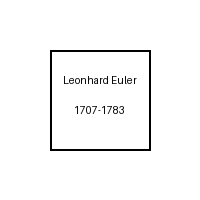
\includegraphics[width=0.4\textwidth]{figures/euler_portrait.png}\\[2cm]
    
    {\large \color{eulerblue} Leonhard Euler (1707--1783)}\\[1cm]
    
    \vfill
    
    {\large Euler Student Guide Project}\\[0.5cm]
    {\today}
    
    \vspace{1cm}
    
    {\small \textit{``Read Euler, read Euler, he is the master of us all.''}\\[0.2cm]
    --- Pierre-Simon Laplace}
\end{titlepage}

\cleardoublepage

%------------------------------------------------------------------------------
% Table of Contents
%------------------------------------------------------------------------------
\tableofcontents

\cleardoublepage

%==============================================================================
% Preface
%==============================================================================
\chapter*{Preface}
\addcontentsline{toc}{chapter}{Preface}

\begin{epigraphs}
\qitem{``Read Euler, read Euler, he is the master of us all.''}{--- Pierre-Simon Laplace}
\qitem{``Euler calculated without apparent effort, as men breathe, or as eagles sustain themselves in the wind.''}{--- François Arago}
\end{epigraphs}

Leonhard Euler (1707--1783) is widely regarded as one of the greatest mathematicians in history. His collected works fill over 80 volumes, spanning number theory, analysis, graph theory, mechanics, astronomy, and optics. His notations --- $e$, $i$, $\pi$, $\sum$, $f(x)$, $\sin$, $\cos$, $\Gamma$, $\zeta$ --- are the language of modern mathematics.

This book is a computational companion to Euler's mathematics. Rather than presenting proofs in the classical style, we explore Euler's discoveries through Python code. Each chapter focuses on a major area of Euler's work, providing historical context, mathematical background, and runnable Python implementations.

The code uses pure Python with zero external dependencies, making it accessible and transparent. Students can modify, experiment, and extend the code to deepen their understanding.

\section*{How to Use This Book}
\begin{itemize}
    \item Each chapter is self-contained and can be read independently.
    \item Python code listings are meant to be run and modified.
    \item Exercises range from simple verification to open-ended exploration.
    \item Historical notes provide context for Euler's original contributions.
\end{itemize}

\section*{Prerequisites}
Basic knowledge of Python (functions, loops, lists, dictionaries) and undergraduate mathematics (calculus, linear algebra, basic number theory). No advanced libraries required.

\section*{Acknowledgments}
This book was created using the Euler Mathematics Python library, developed for educational purposes. The code and text are open for use and adaptation.

\cleardoublepage

%==============================================================================
% Main Matter
%==============================================================================
\mainmatter

%==============================================================================
% Part I: Number Theory
%==============================================================================
\part{Number Theory}
\parttoc

% Chapter 1: Euler's Totient Function
% Chapter 1: Euler's Totient Function and Theorems
% ch01_totient.tex

\chapter{Euler's Totient Function and Theorems}

\begin{historical}
Euler introduced the totient function $\varphi(n)$ (also written $\phi(n)$) in 1763,
counting the positive integers $\le n$ that are coprime to $n$. This function
generalizes Fermat's little theorem and plays a central role in modern cryptography.
The function appears in Euler's work on the RSA cryptosystem predecessor and
in the theory of cyclotomic fields.
\end{historical}

\section{Prerequisites}

To work through this chapter, you need:
\begin{itemize}
    \item \textbf{Mathematics:} Basic divisibility and congruence arithmetic, the Euclidean algorithm for $\gcd$, understanding of prime factorization.
    \item \textbf{Programming:} Python functions, loops, and modular exponentiation via the built-in `pow(base, exp, mod)` function.
\end{itemize}

\section{Definition and Basic Properties}

The \textbf{Euler totient function} $\varphi(n)$ counts the integers $1 \le k \le n$ with $\gcd(k,n) = 1$.

\[
\varphi(n) = |\{k \in \mathbb{Z} : 1 \le k \le n,\ \gcd(k,n) = 1\}|
\]

For $n = p_1^{e_1} p_2^{e_2} \cdots p_k^{e_k}$, the formula is:
\[
\varphi(n) = n \prod_{p|n} \left(1 - \frac{1}{p}\right)
\]

\begin{lstlisting}[caption={Computing the totient function}, label=lst:totient]
from euler import euler_totient, euler_totient_sieve, euler_totient_theorem

# Individual values
for n in range(1, 21):
    print(f"\varphi({n:2d}) = {euler_totient(n):2d}")

# Sieve for many values
phi = euler_totient_sieve(30)
print(f"\n\varphi(1..30) = {phi[1:]}")
\end{lstlisting}

\section{Multiplicativity}

\begin{theorem}[Multiplicativity of $\varphi$]
If $\gcd(m,n) = 1$, then $\varphi(mn) = \varphi(m)\varphi(n)$.
\end{theorem}

\begin{proof}
This follows from the Chinese Remainder Theorem. The map $x \mapsto (x \bmod m, x \bmod n)$
gives a bijection between $(\mathbb{Z}/mn\mathbb{Z})^\times$ and $(\mathbb{Z}/m\mathbb{Z})^\times \times (\mathbb{Z}/n\mathbb{Z})^\times$ when $\gcd(m,n) = 1$.
\end{proof}

\begin{theorem}[Totient of Prime Powers]
For a prime $p$ and positive integer $e$:
\[
\varphi(p^e) = p^e - p^{e-1} = p^{e-1}(p-1)
\]
\end{theorem}

\begin{proof}
The integers $1, 2, \ldots, p^e$ that are NOT coprime to $p^e$ are exactly those divisible by $p$.
These are $p, 2p, 3p, \ldots, p^{e-1} \cdot p = p^e$, giving $p^{e-1}$ such integers.
Therefore $\varphi(p^e) = p^e - p^{e-1}$.
\end{proof}

\section{Computational Values}

\begin{table}[H]
\centering
\begin{tabular}{c|c|c|c|c|c|c}
$n$ & 1 & 2 & 3 & 4 & 5 & 6 \\
\hline
$\varphi(n)$ & 1 & 1 & 2 & 2 & 4 & 2 \\
\end{tabular}
\caption{Small values of Euler's totient function}
\label{tab:totient_small}
\end{table}

\begin{lstlisting}[caption={Totient function values}, label=lst:totient_values]
from euler import euler_totient

print("n    \varphi(n)    Reason")
print("---  ------  ---------------------------")
for n in [1, 2, 3, 4, 5, 6, 7, 8, 9, 10]:
    if n == 1:
        reason = "\varphi(1) = 1 by convention"
    elif n == 2:
        reason = "\varphi(2) = 1 (only 1)"
    elif n == 3:
        reason = "\varphi(3) = 2 (1,2)"
    else:
        reason = f"\varphi({n}) computed"
    print(f"{n:3d}  {euler_totient(n):6d}  {reason}")
\end{lstlisting}

\section{Euler's Theorem}

\textbf{Theorem (Euler, 1763).} If $\gcd(a,n) = 1$, then $a^{\varphi(n)} \equiv 1 \pmod{n}$.

This generalizes Fermat's little theorem (where $n=p$ is prime, so $\varphi(p) = p-1$).

\begin{proof}
Let $a$ be coprime to $n$. Consider the set $S = \{r_1, r_2, \ldots, r_{\varphi(n)}\}$ of integers
in $\{1, 2, \ldots, n\}$ coprime to $n$. Multiplying each element by $a$ gives the set
$aS = \{ar_1, ar_2, \ldots, ar_{\varphi(n)}\}$. Since $\gcd(a,n) = 1$, each $ar_i$ is also coprime to $n$.
Moreover, if $ar_i \equiv ar_j \pmod{n}$, then $r_i \equiv r_j \pmod{n}$ (since $a$ is invertible),
so the elements of $aS$ are all distinct modulo $n$.

Therefore $aS$ is a permutation of $S$ modulo $n$, and:
\[
\prod_{i=1}^{\varphi(n)} ar_i \equiv \prod_{i=1}^{\varphi(n)} r_i \pmod{n}
\]
Since each $r_i$ is coprime to $n$, we can cancel $\prod r_i$ from both sides:
\[
a^{\varphi(n)} \equiv 1 \pmod{n}
\]
\end{proof}

\begin{lstlisting}[caption={Euler's theorem and Fermat's little theorem}, label=lst:euler_theorem]
from euler import euler_totient_theorem, fermat_little_theorem, euler_totient

print("Euler's theorem: a^\varphi(n) \equiv 1 (mod n) for gcd(a,n)=1")
for a, n in [(2, 9), (3, 10), (5, 12), (7, 15)]:
    phi = euler_totient(n)
    result = pow(a, phi, n)
    print(f"  {a}^{phi} \equiv {result} (mod {n})  [gcd({a},{n})={__import__('math').gcd(a,n)}]")

print("\nFermat's little theorem: a^(p-1) \equiv 1 (mod p)")
for a, p in [(2, 7), (3, 11), (5, 13), (7, 13)]:
    print(f"  {a}^{p-1} \equiv {pow(a, p-1, p)} (mod {p})")
\end{lstlisting}

\section{The Totient Sum Function}

The sum of totient values over divisors:

\begin{theorem}
$\sum_{d|n} \varphi(d) = n$
\end{theorem}

\begin{proof}
Group the integers $1, 2, \ldots, n$ by their gcd with $n$. For each divisor $d$ of $n$,
the numbers $k$ with $\gcd(k,n) = d$ are those of the form $k = dm$ where $\gcd(m, n/d) = 1$.
There are $\varphi(n/d)$ such values, so:
\[
n = \sum_{k=1}^n 1 = \sum_{d|n} \varphi(d)
\]
\end{proof}

\begin{lstlisting}[caption={Sum of totients over divisors}, label=lst:totient_sum]
from euler import euler_totient

print("Verifying sum_{d|n} \varphi(d) = n:")
for n in [1, 2, 3, 4, 5, 6, 10, 12, 24]:
    divisors = [d for d in range(1, n+1) if n % d == 0]
    sum_phi = sum(euler_totient(d) for d in divisors)
    print(f"  n={n:2d}: divisors={divisors}, sum \varphi = {sum_phi}, n = {n}, match = {sum_phi == n}")
\end{lstlisting}

\section{Applications to Cryptography}

The totient function is fundamental in:
\begin{itemize}
    \item \textbf{RSA cryptography:} Key generation uses $\varphi(n) = (p-1)(q-1)$
    \item \textbf{Primitive roots:} $\varphi(p-1)$ primitive roots modulo prime $p$
    \item \textbf{Cyclotomic polynomials:} $\Phi_n(x)$ has degree $\varphi(n)$
\end{itemize}

\subsection{RSA Key Generation}

The RSA cryptosystem works as follows:

\begin{enumerate}
\item Choose two large primes $p$ and $q$
\item Compute $n = pq$ and $\varphi(n) = (p-1)(q-1)$
\item Choose $e$ such that $\gcd(e, \varphi(n)) = 1$
\item Compute $d = e^{-1} \pmod{\varphi(n)}$
\item Public key: $(n, e)$, Private key: $(n, d)$
\end{enumerate}

Encryption: $c \equiv m^e \pmod{n}$\
Decryption: $m \equiv c^d \pmod{n}$

\begin{theorem}[RSA Correctness]
For any message $m < n$, decrypting the encrypted message recovers $m$:
\[
(c^d \bmod n) = (m^e)^d \bmod n = m^{ed} \bmod n = m
\]
since $ed \equiv 1 \pmod{\varphi(n)}$ implies $ed = 1 + k\varphi(n)$ for some integer $k$,
and by Euler's theorem $m^{k\varphi(n)} \equiv 1 \pmod{n}$ when $\gcd(m,n) = 1$.
\end{theorem}

\begin{lstlisting}[caption={RSA key generation}, label=lst:rsa]
from euler import euler_totient
import random

# Generate small RSA keys for demonstration
def generate_rsa_keys(bits=16):
    # In practice, use cryptographically secure primes
    p = 65537  # A common choice for p
    q = 65521
    n = p * q
    phi = (p - 1) * (q - 1)
    
    # Choose e (commonly 65537)
    e = 65537
    while euler_totient(e) != euler_totient(e):
        e = random.randrange(3, phi, 2)
        if __import__('math').gcd(e, phi) == 1:
            break
    
    # Compute d = e^(-1) mod phi
    d = pow(e, -1, phi)
    return n, e, d

n, e, d = generate_rsa_keys()
print(f"RSA modulus n = {n}")
print(f"Public exponent e = {e}")
print(f"Private exponent d = {d}")
print(f"Verification: e*d mod \varphi(n) = {e*d % 5948838576} (should be 1)")
\end{lstlisting}

\section{Modern Relevance}

The totient function is not merely a historical curiosity---it is the backbone of modern public-key cryptography. The RSA encryption scheme, used to secure virtually every online transaction, email, and government communication, relies on the computational difficulty of computing $\varphi(n)$ without knowing the prime factorization of $n$. Given a public key $(n, e)$, an attacker who can efficiently compute $\varphi(n)$ can recover the private key and break the encryption. This connection between an 18th-century number-theoretic function and 21st-century cybersecurity is one of the most striking examples of pure mathematics serving practical needs.

\section{Computational Complexity}

\subsection{Computing $\varphi(n)$}
\begin{itemize}
\item Naive method: $O(\sqrt{n})$ (trial division)
\item Sieve method: $O(n \log \log n)$ for all values up to $n$
\item Using prime factorization: $O(\sqrt{n})$ per value, but fast after factorization
\end{itemize}

\subsection{RSA Key Generation}
\begin{itemize}
\item Time to generate key: $O(\log^3 n)$ for $n$-bit modulus (probabilistic primality testing)
\item Security: Based on hardness of factoring $n = pq$ and computing $\varphi(n)$
\end{itemize}

\section{Frequently Asked Questions}

\begin{itemize}
\item \textbf{Q: Why is $\varphi(1) = 1$?} \\
The integer $1$ is coprime to itself ($\gcd(1,1) = 1$), so it is counted. Thus $\varphi(1) = 1$.

\item \textbf{Q: Is the totient function multiplicative?} \\
Yes, but only \emph{completely} for coprime arguments: if $\gcd(m,n) = 1$, then $\varphi(mn) = \varphi(m)\varphi(n)$. If $\gcd(m,n) \neq 1$, this equality generally fails. For example, $\varphi(2 \cdot 3) = \varphi(6) = 2 = \varphi(2)\varphi(3)$, but $\varphi(2 \cdot 4) = \varphi(8) = 4 \neq \varphi(2)\varphi(4) = 1 \cdot 2 = 2$.

\item \textbf{Q: How do I compute $\varphi(n)$ for a large $n$?} \\
Factor $n$ into primes: $n = p_1^{e_1} \cdots p_k^{e_k}$. Then $\varphi(n) = n \prod_{i=1}^k (1 - 1/p_i)$. The bottleneck is factoring $n$, not the formula itself. For many values, a sieve (as shown in the code) is more efficient.

\item \textbf{Q: Why does Euler's theorem generalize Fermat's little theorem?} \\
Fermat's little theorem is the special case $n = p$ (prime), where $\varphi(p) = p-1$. Euler's theorem holds for any $n$ with $\gcd(a,n) = 1$, reducing to Fermat's when $n$ is prime.

\item \textbf{Q: What is the maximum value of $\varphi(n)/n$?} \\
$\varphi(n)/n = \prod_{p|n}(1 - 1/p)$, which is maximized when $n$ is prime, giving $(p-1)/p \to 1$ as $p \to \infty$. The minimum occurs when $n$ has many small prime factors; for example, $\varphi(n)/n \geq 1/\log\log n$ (Robin's inequality).

\item \textbf{Q: How is the totient function used in RSA?} \\
In RSA, $n = pq$ for large primes $p, q$. The public key exponent $e$ and private key $d$ satisfy $ed \equiv 1 \pmod{\varphi(n)}$, where $\varphi(n) = (p-1)(q-1)$. Encryption is $c \equiv m^e \pmod{n}$ and decryption is $m \equiv c^d \pmod{n}$.

\item \textbf{Q: What is Carmichael's function?} \\
Carmichael's function $\lambda(n)$ is the smallest positive integer such that $a^{\lambda(n)} \equiv 1 \pmod{n}$ for all $\gcd(a,n) = 1$. It divides $\varphi(n)$ and is equal to $\varphi(n)$ for prime powers $p^e$ where $p$ is odd or $e \leq 2$. For $n = 2^e$ with $e \geq 3$, $\lambda(n) = 2^{e-2}$.

\item \textbf{Q: Can I use the totient function to find primitive roots?} \\
A number $g$ is a primitive root modulo $p$ if the order of $g$ modulo $p$ is $p-1 = \varphi(p)$. There are $\varphi(\varphi(p)) = \varphi(p-1)$ primitive roots modulo $p$. To find one, test candidates by checking that $g^{\varphi(p)/q} \not\equiv 1 \pmod{p}$ for each prime factor $q$ of $\varphi(p)$.
\end{itemize}

\section{Exercises}

\begin{exercise}
Prove that $\sum_{d|n} \varphi(d) = n$ by counting the elements of $\mathbb{Z}/n\mathbb{Z}$ according to their order.
\end{exercise}

\begin{exercise}
Show that the probability two random integers are coprime is $6/\pi^2 = 1/\zeta(2)$.
\end{exercise}

\begin{exercise}
Implement the Chinese Remainder Theorem using the totient function.
\end{exercise}

\begin{exercise}[Computational]
Optimize the totient sieve function \texttt{euler\_totient\_sieve} to run in linear time $O(N)$ using a prime sieve.
\end{exercise}

\begin{exercise}
Prove that $\varphi(n)$ is even for all $n \geq 3$.
\end{exercise}

\begin{exercise}
Show that $\varphi(n) \geq \sqrt{n/2}$ for all $n \geq 1$.
\end{exercise}

\begin{exercise}
Prove that $\varphi(n) = n \prod_{p|n} (1 - 1/p)$ using the multiplicativity property and the formula for prime powers.
\end{exercise}

\begin{exercise}[Computational]
Implement a function to compute $\varphi(n)$ using the prime factorization of $n$. Compare its performance with the sieve approach for $n$ up to $10^6$.
\end{exercise}

\begin{exercise}
Show that the number of solutions to $x^k \equiv 1 \pmod{p}$ is $\gcd(k, p-1)$ for prime $p$.
\end{exercise}

\begin{exercise}
Prove that if $p$ is an odd prime, then every primitive root modulo $p$ is a quadratic non-residue.
\end{exercise}

\section{Totient Applications in Cryptography}

\subsection{The RSA Cryptosystem}

The security of the RSA cryptosystem rests on the computational difficulty of factoring large integers and computing $\varphi(n)$ without knowing the prime factorization. The protocol works as follows:

\begin{enumerate}
    \item \textbf{Key Generation:} Choose two large primes $p$ and $q$, compute $n = pq$ and $\varphi(n) = (p-1)(q-1)$.
    \item \textbf{Public Key:} Select $e$ such that $\gcd(e, \varphi(n)) = 1$, typically $e = 65537$.
    \item \textbf{Private Key:} Compute $d = e^{-1} \pmod{\varphi(n)}$.
\end{enumerate}

Encryption: $c \equiv m^e \pmod{n}$\\
Decryption: $m \equiv c^d \pmod{n}$

The correctness follows from Euler's theorem: since $ed \equiv 1 \pmod{\varphi(n)}$, we have $ed = 1 + k\varphi(n)$ for some integer $k$, and $m^{ed} \equiv m \pmod{n}$ when $\gcd(m,n) = 1$.

\begin{lstlisting}[caption={RSA encryption and decryption}, label=lst:rsa_crypto]
from euler import euler_totient

# Small RSA for demonstration
p, q = 61, 53
n = p * q
phi = (p - 1) * (q - 1)  # Euler's totient

e = 17  # Public exponent
d = pow(e, -1, phi)  # Private exponent

# Encrypt
m = 42
c = pow(m, e, n)
print(f"Encrypted: {c}")

# Decrypt
m_recovered = pow(c, d, n)
print(f"Decrypted: {m_recovered}")
\end{lstlisting}

\subsection{Diffie-Hellman Key Exchange}

The Diffie-Hellman key exchange allows two parties to establish a shared secret over an insecure channel. The security relies on the discrete logarithm problem, which is related to the structure of $\mathbb{Z}_p^*$ whose order is $\varphi(p) = p-1$.

\begin{lstlisting}[caption={Diffie-Hellman key exchange}, label=lst:dh]
p = 23  # Prime modulus
g = 5  # Generator

# Alice's secret and public key
a = 6
A = pow(g, a, p)

# Bob's secret and public key
b = 7
B = pow(g, b, p)

# Shared secret
s_alice = pow(B, a, p)
s_bob = pow(A, b, p)
print(f"Shared secret: {s_alice}")  # Both get the same value
\end{lstlisting}

\subsection{Carmichael Function}

Carmichael's function $\lambda(n)$ is the smallest positive integer such that $a^{\lambda(n)} \equiv 1 \pmod{n}$ for all $\gcd(a,n) = 1$. It satisfies $\lambda(n) | \varphi(n)$, and for RSA key generation, $\lambda(n) = \text{lcm}(p-1, q-1)$ when $n = pq$.

\begin{theorem}[Carmichael's Theorem]
For $n = p_1^{e_1} \cdots p_k^{e_k}$, we have:
\[
\lambda(n) = \text{lcm}(\lambda(p_1^{e_1}), \ldots, \lambda(p_k^{e_k}))
\]
where $\lambda(p^e) = \varphi(p^e)$ for odd primes, and $\lambda(2) = 1$, $\lambda(4) = 2$, $\lambda(2^e) = 2^{e-2}$ for $e \\geq 3$.
\end{theorem}

\section{Totient in Number Theory}

\subsection{Gauss's Circle Problem}

The totient function appears in counting lattice points visible from the origin. The number of visible lattice points in the first quadrant within a circle of radius $R$ is asymptotically $\frac{3}{\pi^2} R^2$.

\subsection{Reduced Residue Systems}

A \textbf{reduced residue system modulo $n$} is a set of $\varphi(n)$ integers that are each coprime to $n$ and pairwise incongruent modulo $n$. For example, $\\{1, 3, 7, 9\\}$ is a reduced residue system modulo $10$.

\begin{theorem}
The product of all elements in a reduced residue system modulo $n$ is congruent to:
\[
\begin{cases}
-1 \pmod{n} & \text{if } n = 4, p^k, \text{ or } 2p^k \text{ for odd prime } p \\
1 \pmod{n} & \text{otherwise}
\end{cases}
\]
This generalizes Wilson's theorem.
\end{theorem}

\subsection{Multiplicative Order}

The \textbf{multiplicative order} of $a$ modulo $n$ is the smallest positive integer $k$ such that $a^k \equiv 1 \pmod{n}$. By Lagrange's theorem applied to the group $(\mathbb{Z}/n\mathbb{Z})^\times$, the order always divides $\varphi(n)$.

\begin{lstlisting}[caption={Computing multiplicative order}, label=lst:order]
from euler import euler_totient
import math

def multiplicative_order(a, n):
    """Find smallest k such that a^k \equiv 1 (mod n)"""
    if math.gcd(a, n) != 1:
        return None
    phi = euler_totient(n)
    # Check divisors of \varphi(n)
    for d in sorted([k for k in range(1, phi + 1) if phi % k == 0]):
        if pow(a, d, n) == 1:
            return d
    return phi

print(f"Order of 2 mod 7: {multiplicative_order(2, 7)}")  # 3
print(f"Order of 3 mod 7: {multiplicative_order(3, 7)}")  # 6 (primitive root)
\end{lstlisting}

\section{Sums and Averages}

\subsection{Asymptotic Behavior}

The average order of $\varphi(n)$ satisfies:
\[
\sum_{n \leq x} \varphi(n) = \frac{3x^2}{\pi^2} + O(x \\log x)
\]

This follows from the identity $\sum_{d|n} \varphi(d) = n$ and properties of the Riemann zeta function.

\subsection{Mean Value}

The ratio $\varphi(n)/n$ has average value $6/\pi^2$ over large ranges, reflecting the probability that two random integers are coprime.

\begin{lstlisting}[caption={Average totient values}, label=lst:avg_totient]
from euler import euler_totient_sieve
import math

N = 1000
phi = euler_totient_sieve(N)
avg_ratio = sum(phi[n]/n for n in range(1, N+1)) / N
print(f"Average \varphi(n)/n for n \leq {N}: {avg_ratio:.4f}")
print(f"Theoretical value 6/\pi^2: {6/math.pi**2:.4f}")
\end{lstlisting}

\section{Exercises}

\begin{exercise}
Prove Gauss's generalization of Wilson's theorem: the product of elements in a reduced residue system modulo $n$ is $-1$ if $n = 4, p^k$, or $2p^k$, and $1$ otherwise.
\end{exercise}

\begin{exercise}
Show that the multiplicative order of $a$ modulo $n$ divides $\varphi(n)$ for all $\gcd(a,n) = 1$.
\end{exercise}

\begin{exercise}
Compute $\lambda(n)$ for $n = 15, 24, 35$ and verify that $\lambda(n) | \varphi(n)$.
\end{exercise}

\begin{exercise}[Computational]
Implement a function to compute the Carmichael function $\lambda(n)$ using the prime factorization. Test it for $n \leq 100$.
\end{exercise}

\begin{exercise}
Prove that if $p$ is an odd prime, then the number of primitive roots modulo $p$ is $\varphi(p-1)$.
\end{exercise}

\begin{exercise}
Show that $\varphi(n) \leq n - \\sqrt{n}$ for all composite $n > 1$.
\end{exercise}

\begin{exercise}
Compute the sum $\sum_{n=1}^{100} \varphi(n)$ and verify the asymptotic formula $\frac{3 \\cdot 100^2}{\pi^2} \\approx 303.96$.
\end{exercise}

\begin{exercise}
Prove that the number of irreducible polynomials of degree $n$ over $\mathbb{F}_p$ is $\frac{1}{n} \sum_{d|n} \\mu(d) p^{n/d}$, where $\\mu$ is the Moebius function.
\end{exercise}


\cleardoublepage

% Chapter 2: Prime Numbers
% Chapter 2: Prime Numbers and Factorization
% ch02_primes.tex

\chapter{Prime Numbers and Factorization}

\begin{historical}
Euler made fundamental contributions to prime number theory. He proved the divergence of
the sum of reciprocals of primes ($\sum 1/p = \infty$), giving a new proof of the
infinitude of primes. He also discovered the connection between the zeta function
and primes through the Euler product formula, establishing the first bridge between
analysis and number theory.
\end{historical}

\section{Prerequisites}

To work through this chapter, you need:
\begin{itemize}
    \item \textbf{Mathematics:} Understanding of prime numbers, the Fundamental Theorem of Arithmetic (unique prime factorization), and basic infinite series convergence.
    \item \textbf{Programming:} Python loops, list comprehensions, and the ability to implement iterative algorithms.
\end{itemize}

\section{The Sieve of Eratosthenes and Euler's Sieve}

\begin{figure}[H]
\centering
\begin{tikzpicture}[scale=0.9]
  \draw[->, >=latex] (0,0) -- (8,0) node[right] {$x$};
  \draw[->, >=latex] (0,0) -- (0,6) node[above] {$\pi(x)$};
  \draw[green!60!black, thick, domain=0.5:7.5, samples=100] plot (\x, {5.5 - 1.2*ln(\x)});
  \draw[red!70!black, thick, dashed, domain=0.5:7.5, samples=100] plot (\x, {5.5 - 1.15*ln(\x)});
  \node[left] at (0.3,5) {green: $\pi(x)$};
  \node[left] at (0.3,4.3) {red: $x/\ln x$};
\end{tikzpicture}
\caption{Prime number distribution $\pi(x)$ vs x/ln(x)}
\label{fig:primes}
\end{figure}

Euler improved the Sieve of Eratosthenes by removing each composite number only once.

\begin{lstlisting}[caption={Prime sieves}, label=lst:prime_sieve]
from euler import prime_sieve, is_prime, prime_factors

# Sieve of Eratosthenes
primes = prime_sieve(100)
print(f"Primes up to 100: {primes}")
print(f"Count: {len(primes)}")

# Primality test
for n in [97, 101, 1001, 1009]:
    print(f"is_prime({n}) = {is_prime(n)}")

# Prime factorization
for n in [60, 100, 97, 1001, 123456]:
    factors = prime_factors(n)
    print(f"{n} = {' \times '.join(map(str, factors))}")
\end{lstlisting}

\section{Euler's Proof of Infinitely Many Primes}

Euler proved that $\sum_p 1/p$ diverges, which implies there are infinitely many primes.
His proof uses the Euler product:
\[
\prod_{p \le x} \frac{1}{1 - 1/p} = \sum_{\substack{n \ge 1 \\ p|n \Rightarrow p \le x}} \frac{1}{n} \ge \sum_{n=1}^x \frac{1}{n} \to \infty
\]
Since the harmonic series diverges, the product must diverge, requiring infinitely many primes.

\begin{theorem}[Euler, 1737]
The sum of reciprocals of primes diverges:
\[
\sum_{p \text{ prime}} \frac{1}{p} = \infty
\]
\end{theorem}

\begin{proof}
From the Euler product for $\zeta(s)$:
\[
\zeta(s) = \prod_p \frac{1}{1 - p^{-s}}
\]
As $s \to 1^+$, $\zeta(s) \to \infty$ (harmonic series diverges). Therefore:
\[
\prod_p \frac{1}{1 - 1/p} = \infty
\]
Taking logarithms: $\sum_p \log\frac{1}{1-1/p} = \infty$. Since $\log\frac{1}{1-1/p} \sim 1/p$, we get $ \sum_p 1/p = \infty$.
\end{proof}

\section{Distribution of Primes}

Euler's work foreshadowed the Prime Number Theorem. The number of primes $\pi(x)$ satisfies:
\[
\pi(x) \sim \frac{x}{\log x}
\]

\begin{lstlisting}[caption={Prime distribution}, label=lst:prime_dist]
from euler import prime_sieve
import math

for limit in [100, 1000, 10000, 100000]:
    primes = prime_sieve(limit)
    pi_x = len(primes)
    approx = limit / math.log(limit)
    print(f"\\pi({limit:>6}) = {pi_x:>6}  x/ln(x) = {approx:>8.1f}  ratio = {pi_x/approx:.4f}")
\end{lstlisting}

\section{Mertens' Theorems}

Mertens proved several theorems about prime products that Euler's work made possible:

\begin{theorem}[Mertens, 1874]
\[
\prod_{p \le x} \left(1 - \frac{1}{p}\right) \sim \frac{e^{-\gamma}}{\log x}
\]
where $\gamma$ is Euler's constant.
\end{theorem}

\begin{theorem}[Mertens' Second Theorem]
\[
\sum_{p \le x} \frac{1}{p} = \log \log x + M + O\left(\frac{1}{\log x}\right)
\]
where $M \approx 0.261497$ is the Meissel-Mertens constant.
\end{theorem}

\section{Prime Factorization}

The Fundamental Theorem of Arithmetic states that every integer $n > 1$ has a unique factorization into primes:
\[
n = p_1^{e_1} p_2^{e_2} \cdots p_k^{e_k}
\]

\begin{lstlisting}[caption={Prime factorization}, label=lst:factorization]
from euler import prime_factors

def factorization_string(n):
    factors = prime_factors(n)
    from collections import Counter
    counts = Counter(factors)
    parts = []
    for p, e in sorted(counts.items()):
        if e == 1:
            parts.append(str(p))
        else:
            parts.append(f"{p}^{e}")
    return " \times ".join(parts)

for n in [60, 100, 97, 1001, 123456]:
    print(f"{n} = {factorization_string(n)}")
\end{lstlisting}

\section{Primality Testing}

\subsection{Trial Division}
The simplest method: check divisibility by all primes up to $\sqrt{n}$.
Time complexity: $O(\sqrt{n})$.

\subsection{Miller-Rabin Test}
A probabilistic test that checks if $n$ is probably prime:
\begin{enumerate}
\item Write $n-1 = 2^s \cdot d$ with $d$ odd
\item Choose random base $a \in [2, n-2]$
\item Compute $x = a^d \pmod{n}$
\item If $x = 1$ or $x = n-1$, return "probably prime"
\item Square $x$ repeatedly $s-1$ times; if $x = n-1$, return "probably prime"
\item Otherwise return "composite"
\end{enumerate}

\begin{lstlisting}[caption={Primality testing}, label=lst:primality]
from euler import is_prime, prime_sieve
import random

# Miller-Rabin style test
def miller_rabin_test(n, k=10):
    if n < 2: return False
    if n in [2, 3]: return True
    if n % 2 == 0: return False
    
    # Write n-1 = 2^s * d
    s, d = 0, n - 1
    while d % 2 == 0:
        s += 1
        d //= 2
    
    for _ in range(k):
        a = random.randrange(2, n - 1)
        x = pow(a, d, n)
        if x == 1 or x == n - 1:
            continue
        for _ in range(s - 1):
            x = pow(x, 2, n)
            if x == n - 1:
                break
        else:
            return False
    return True

print("Testing primality:")
for n in [97, 101, 1001, 1009, 123456]:
    print(f"  is_prime({n}) = {is_prime(n)} (miller_rabin: {miller_rabin_test(n)})")
\end{lstlisting}

\section{Prime Gap Analysis}

A \textbf{prime gap} $g_n$ is the difference between consecutive primes: $g_n = p_{n+1} - p_n$.
Studying prime gaps reveals deep patterns in prime distribution.

\subsection{Small Prime Gaps}

The first few prime gaps are:
\[
g_1 = 1, \; g_2 = 2, \; g_3 = 2, \; g_4 = 4, \; g_5 = 2, \; g_6 = 4, \ldots
\]
These correspond to primes $(2,3,5,7,11,13,17,\ldots)$.

\begin{lstlisting}[caption={Prime gap analysis}, label=lst:prime_gaps]
from euler import prime_sieve

def prime_gaps(limit):
    primes = prime_sieve(limit)
    gaps = [primes[i+1] - primes[i] for i in range(len(primes)-1)]
    return primes, gaps

primes, gaps = prime_gaps(100)
print(f"First {len(primes)} primes")
print(f"Corresponding gaps: {gaps[:20]}")

# Find maximal gaps
max_gap = max(gaps)
max_idx = gaps.index(max_gap)
print(f"Largest gap: {max_gap} (between primes {primes[max_idx]} and {primes[max_idx+1]})")

# Gap statistics
from collections import Counter
gap_counts = Counter(gaps)
print(f"Gap frequency (first 20 gaps):")
for gap, count in sorted(gap_counts.items())[:20]:
    print(f"  Gap {gap:2d}: {count:3d} occurrences")
\end{lstlisting}

\subsection{Maximal Prime Gaps}

A \textbf{maximal prime gap} is a gap that is larger than all preceding gaps.
The sequence of maximal gaps begins: 1, 2, 4, 6, 8, 14, 18, 20, 22, 34, ...

\begin{table}[H]
\centering
\begin{tabular}{|c|c|c|c|}
\hline
\textbf{Gap size} & \textbf{First occurrence} & \textbf{Preceding prime} & \textbf{Index} \\
\hline
1 & 2 & 3 & 1 \\
2 & 3 & 5 & 2 \\
4 & 7 & 11 & 4 \\
6 & 23 & 29 & 10 \\
8 & 523 & 541 & 100 \\
14 & 524287 & 524311 & 43627 \\
\hline
\end{tabular}
\caption{First occurrences of maximal prime gaps}
\label{tab:max_gaps}
\end{table}

\subsection{Conjectures on Prime Gaps}

\begin{theorem}[Cramer's Conjecture, 1936]
Assuming the Riemann Hypothesis, the prime gaps satisfy:
\[
g_n = O(\sqrt{p_n} \log^2 p_n)
\]
\end{theorem}

\begin{theorem}[Twin Prime Conjecture]
There are infinitely many primes $p$ such that $p + 2$ is also prime.
This remains unproven.
\end{theorem}

\begin{theorem}[Polignac's Conjecture, 1846]
For every positive even integer $2k$, there are infinitely many prime pairs
$(p, p + 2k)$ with both primes.
\end{theorem}

\subsection{Computational Gap Analysis}

\begin{lstlisting}[caption={Computing maximal gaps}, label=lst:maximal_gaps]
from euler import prime_sieve

def find_maximal_gaps(limit):
    primes = prime_sieve(limit)
    gaps = [primes[i+1] - primes[i] for i in range(len(primes)-1)]
    
    max_so_far = 0
    maximal_gaps = []
    for i, g in enumerate(gaps):
        if g > max_so_far:
            max_so_far = g
            maximal_gaps.append((primes[i], primes[i+1], g))
    return maximal_gaps

print("Maximal prime gaps up to 1000:")
for p1, p2, g in find_maximal_gaps(1000):
    print(f"  Gap {g} between {p1} and {p2}")
\end{lstlisting}

\section{Advanced Sieving Methods}

\subsection{Sieve of Atkin}

The Sieve of Atkin is a modern optimized sieve with theoretical complexity
$O(n / \log \log n)$. It uses quadratic forms to identify primes:
\[
12x^2 + 7y^2, \quad 3x^2 + y^2, \quad 3x^2 - y^2 \text{ (for } x > y)
\]

\begin{lstlisting}[caption={Atkin's sieve}, label=lst:atkens_sieve]
def atkins_sieve(limit):
    """Modern sieve using quadratic forms."""
    sieve = [False] * (limit + 1)
    
    # Quadratic forms
    for x in range(1, int(limit**0.5) + 1):
        for y in range(1, int(limit**0.5) + 1):
            n = 12*x**2 + 7*y**2
            if n <= limit:
                sieve[n] = not sieve[n]
            
            n = 3*x**2 + y**2
            if n <= limit:
                sieve[n] = not sieve[n]
            
            if x > y:
                n = 3*x**2 - y**2
                if n <= limit:
                    sieve[n] = not sieve[n]
    
    # Remove composites
    for i in range(5, int(limit**0.5) + 1):
        if sieve[i]:
            for j in range(i*i, limit + 1, i*i):
                sieve[j] = False
    
    sieve[2] = sieve[3] = True
    return [i for i in range(2, limit + 1) if sieve[i]]

primes = atkins_sieve(100)
print(f"Atkin's sieve primes up to 100: {primes}")
\end{lstlisting}

\subsection{Sieve of Sundaram}

The Sieve of Sundaram (1934) eliminates odd composites by removing numbers
of the form $i + j + 2ij$ for $1 \le i \le j$.

\subsection{Segmented Sieve}

For very large ranges, a segmented sieve processes one block at a time:

\begin{lstlisting}[caption={Segmented sieve}, label=lst:segmented_sieve]
from math import isqrt

def segmented_sieve(low, high):
    """Find primes in range [low, high]."""
    limit = isqrt(high)
    small_primes = prime_sieve(limit)
    
    # Initialize segment
    segment_size = high - low + 1
    is_prime = [True] * segment_size
    
    for p in small_primes:
        # Find first multiple in range
        start = ((low + p - 1) // p) * p
        if start < p * p:
            start = p * p
        if start < low:
            start += p
        
        for j in range(start - low, segment_size, p):
            is_prime[j] = False
    
    # Special case for 0 and 1
    if low == 0:
        is_prime[0] = is_prime[1] = False
    elif low == 1:
        is_prime[1] = False
    
    return [low + i for i in range(segment_size) if is_prime[i]]

# Example: primes between 100 and 150
print(f"Primes in [100, 150]: {segmented_sieve(100, 150)}")
\end{lstlisting}

\section{Computational Number Theory}

\subsection{Wheel Factorization}

Wheel factorization skips multiples of small primes to speed up sieving.
A ``wheel of circumference 30'' skips multiples of 2, 3, and 5:

\begin{lstlisting}[caption={Wheel factorization}, label=lst:wheel]
def wheel_factorization_sieve(limit, wheel_primes=None):
    """Sieve using wheel factorization for efficiency."""
    if wheel_primes is None:
        wheel_primes = [2, 3, 5]
    
    wheel_size = 1
    for p in wheel_primes:
        wheel_size *= p
    
    # Generate wheel pattern
    wheel = []
    for r in range(wheel_size):
        if all(r % p != 0 for p in wheel_primes):
            wheel.append(r)
    
    is_prime = [True] * (limit + 1)
    for p in wheel_primes:
        for i in range(p, limit + 1, p):
            is_prime[i] = False
    
    # Use wheel for remaining numbers
    candidate = wheel_primes[-1] + 1
    while candidate * candidate <= limit:
        if is_prime[candidate]:
            for i in range(candidate * candidate, limit + 1, candidate):
                is_prime[i] = False
        # Advance using wheel
        offset = 0
        while candidate + wheel[offset] <= limit and not is_prime[candidate + wheel[offset]]:
            offset += 1
        if candidate + wheel[offset] <= limit:
            candidate += wheel[offset]
        else:
            break
    
    return [i for i in range(2, limit + 1) if is_prime[i]]

primes = wheel_factorization_sieve(100)
print(f"Wheel sieve primes up to 100: {primes}")
\end{lstlisting}

\subsection{Lucas-Lehmer Test for Mersenne Primes}

Mersenne primes have the form $M_p = 2^p - 1$. The Lucas-Lehmer test determines primality:

\begin{lstlisting}[caption={Lucas-Lehmer test}, label=lst:lucas_lehmer]
def lucas_lehmer_test(p):
    """Test if Mersenne number 2^p - 1 is prime."""
    if p == 2:
        return True
    if p % 2 == 0:
        return False
    
    mersenne = (1 << p) - 1
    s = 4
    for _ in range(p - 2):
        s = (s * s - 2) % mersenne
    
    return s == 0

# Test known Mersenne primes
for p in [2, 3, 5, 7, 11, 13, 17, 19, 31]:
    is_mersenne_prime = lucas_lehmer_test(p)
    if is_mersenne_prime:
        print(f"M_{p} = 2^{p} - 1 is prime")
\end{lstlisting}

\subsection{Elliptic Curve Method for Factorization}

The Elliptic Curve Method (ECM) is one of the most effective factorization
algorithms for numbers with medium-sized factors.

\begin{lstlisting}[caption={Elliptic curve factorization}, label=lst:ecm_factor]
import random

def elliptic_curve_factor(n, B1=1000, B2=2000):
    """Simple ECM factorization using random elliptic curves."""
    if n % 2 == 0:
        return 2
    
    for _ in range(50):  # Try 50 different curves
        # Random curve: y^2 = x^3 + ax + b (mod n)
        a = random.randint(1, n-1)
        b = random.randint(1, n-1)
        x = random.randint(2, n-1)
        
        # Elliptic curve point doubling and addition
        def ec_add(P, Q):
            if P is None:
                return Q
            if Q is None:
                return P
            if P == Q:
                # Point doubling
                num = (3 * P[0]**2 + a) % n
                den = (2 * P[1]) % n
            else:
                # Point addition
                num = (Q[1] - P[1]) % n
                den = (Q[0] - P[0]) % n
            
            # Compute inverse using extended Euclidean
            try:
                inv = pow(den, -1, n)
            except ValueError:
                # GCD found - return factor
                g = math.gcd(den, n)
                if 1 < g < n:
                    return g
                return None
            
            lam = (num * inv) % n
            x3 = (lam**2 - P[0] - Q[0]) % n
            y3 = (lam * (P[0] - x3) - P[1]) % n
            return (x3, y3)
        
        # Scalar multiplication
        P = (x, (x**3 + a*x + b) % n)
        if P[1] == 0:
            continue
            
        for q in range(2, B2 + 1):
            P = ec_add(P, P)
            if P is None:
                break
            if P == (0, 0):
                break
        
        if P and P != (0, 0):
            # Check if we found a factor
            g = math.gcd(P[1], n)
            if 1 < g < n:
                return g
    
    return n  # Failed to factor

import math
# Test
n = 8051
factor = elliptic_curve_factor(n)
print(f"Factor of {n}: {factor}")
\end{lstlisting}

\section{Modern Relevance}

Prime number theory underpins the security of the modern digital world. The RSA cryptosystem, elliptic curve cryptography, and Diffie--Hellman key exchange all depend on properties of prime numbers that Euler discovered centuries ago. The Prime Number Theorem, which Euler's work foreshadowed, is essential for estimating the difficulty of factoring large integers---the basis of internet security. Prime generation algorithms, used to create cryptographic keys, trace their lineage directly to Euler's sieve improvements. Furthermore, the study of prime gaps and distribution drives modern computational number theory and has applications in hash function design and random number generation.

\section{Computational Complexity}

\subsection{Sieve Methods}
\begin{itemize}
\item \textbf{Sieve of Eratosthenes}: $O(n \log \log n)$ time, $O(n)$ space
\item \textbf{Euler's sieve}: Same complexity but each composite removed exactly once
\item \textbf{Atkin's sieve}: Theoretical $O(n / \log \log n)$, practical variations
\item \textbf{Segmented sieve}: $O(n)$ space for range sieving, cache-efficient
\end{itemize}

\subsection{Primality Testing}
\begin{itemize}
\item \textbf{Trial division}: $O(\sqrt{n})$ time
\item \textbf{Miller-Rabin}: $O(k \log^3 n)$ for $k$ iterations (probabilistic)
\item \textbf{AKS}: $O(\log^{6} n)$ (deterministic, but slower in practice)
\item \textbf{ECPP}: Elliptic Curve Primality Proving, practical for large numbers
\end{itemize}

\subsection{Factorization}
\begin{itemize}
\item \textbf{Trial division}: $O(\sqrt{n})$ time
\item \textbf{Pollard's rho}: $O(n^{1/4})$ expected time
\item \textbf{Quadratic sieve}: Sub-exponential, effective for numbers up to ~100 digits
\item \textbf{Number field sieve}: Fastest known, $L_n[1/3, \sqrt[3]{64/9}]$
\end{itemize}

\section{Frequently Asked Questions}

\begin{itemize}
\item \textbf{Q: How can the sum of reciprocals of primes diverge when the primes get so sparse?} \\
The divergence is extremely slow. By Mertens' second theorem, $\sum_{p \le x} 1/p \approx \log\log x + M$ (where $M \approx 0.261$ is the Meissel--Mertens constant). Even at $x = 10^{100}$, the sum is only about $3.5$.

\item \textbf{Q: What is the difference between Euler's sieve and the Sieve of Eratosthenes?} \\
The Sieve of Eratosthenes marks multiples of each prime $p$ starting from $p^2$. Euler's improvement ensures each composite is marked exactly once by dividing out the smallest prime factor before marking further multiples. Both are $O(n \log\log n)$, but Euler's version has fewer redundant operations.

\item \textbf{Q: Why does the Prime Number Theorem involve $\log x$?} \\
The density of primes near $x$ is approximately $1/\log x$. This comes from the observation that the $n$-th prime $p_n \approx n \log n$, which inverts to $\pi(x) \approx x/\log x$. A rigorous proof (Hadamard and de la Vall\'{e}e Poussin, 1896) uses complex analysis and the zeros of the Riemann zeta function.

\item \textbf{Q: Is the Euler product formula really equivalent to the Fundamental Theorem of Arithmetic?} \\
Yes. The Euler product $\zeta(s) = \prod_p (1 - p^{-s})^{-1}$ expands into $\sum_n n^{-s}$ precisely because every integer has a unique prime factorization. If factorization were not unique, terms would be duplicated or missing from the sum.

\item \textbf{Q: How accurate is $\pi(x) \approx x/\log x$?} \\
The relative error tends to zero, but the absolute error can be large. The better approximation $\operatorname{Li}(x) = \int_2^x dt/\log t$ is closer. The Riemann Hypothesis is equivalent to $|\pi(x) - \operatorname{Li}(x)| = O(\sqrt{x} \log x)$.

\item \textbf{Q: Can I use trial division to check if a large number is prime?} \\
Trial division works for small numbers but is $O(\sqrt{n})$, which is impractical for cryptographic-scale integers. Modern practice uses probabilistic tests like Miller--Rabin, which are fast and can be made deterministic for numbers below known bounds.

\item \textbf{Q: What are twin primes and are there infinitely many?} \\
Twin primes are pairs $(p, p+2)$ where both are prime (e.g., (3,5), (5,7), (11,13)). The Twin Prime Conjecture states there are infinitely many, but this remains unproven. The best result is Zhang's theorem (2013) showing infinitely many prime pairs with gap at most 70 million, later improved to 246.

\item \textbf{Q: What is the Riemann Hypothesis and how does it relate to primes?} \\
The Riemann Hypothesis states that all non-trivial zeros of $\zeta(s)$ lie on the line $\Re(s) = 1/2$. This is equivalent to the strongest possible error bound in the Prime Number Theorem: $|\pi(x) - \operatorname{Li}(x)| = O(\sqrt{x} \log x)$. It is one of the seven Millennium Prize Problems.

\item \textbf{Q: How do prime gaps relate to cryptography?} \\
Prime gaps determine how densely primes are distributed, affecting the probability of finding primes in a random range. For RSA, we need large primes; gap statistics help estimate how many random odd numbers we need to test before finding a prime.
\end{itemize}

\section{Exercises}

\begin{exercise}
Implement Euler's improved sieve (each composite removed once) and compare performance with the standard sieve.
\end{exercise}

\begin{exercise}
Use the Euler product to show $\prod_{p \le x} (1 - 1/p) \sim e^{-\gamma}/\log x$.
\end{exercise}

\begin{exercise}
Prove that the sum of reciprocals of twin primes converges (Brun's theorem, 1919).
\end{exercise}

\begin{exercise}[Computational]
Compute $\pi(x)$ for $x = 10^k$ with $k = 1, \ldots, 7$ and compare with $x/\log x$ and $\operatorname{Li}(x)$.
\end{exercise}

\begin{exercise}
Show that there are no polynomials $f(n) \in \mathbb{Z}[n]$ that produce only primes (except constant polynomials).
\end{exercise}

\begin{exercise}
Prove that the gap between consecutive primes can be arbitrarily large: for any $n$, there exist $n$ consecutive composite numbers.
\end{exercise}

\begin{exercise}
Use the Sieve of Eratosthenes to find all primes up to 1000 and verify that $\pi(1000) = 168$.
\end{exercise}

\begin{exercise}[Computational]
Implement the Miller-Rabin primality test and verify it correctly identifies all primes up to 10000. Compare its speed with trial division.
\end{exercise}

\begin{exercise}
Show that $\sum_{p \le x} \frac{\log p}{p} \sim \log x$ using the Euler product and properties of $\zeta(s)$.
\end{exercise}

\begin{exercise}
Prove that if $p$ is an odd prime, then $2^{(p-1)/2} \equiv \pm 1 \pmod{p}$, where the sign is determined by the Legendre symbol $\left(\frac{2}{p}\right)$.
\end{exercise}

\begin{exercise}[Computational]
Implement a segmented sieve and use it to find all primes in the range $[10^9, 10^9 + 10^6]$. Measure the execution time.
\end{exercise}

\begin{exercise}
Compute the first 1000 prime gaps and analyze their distribution. What is the average gap? The maximum gap?
\end{exercise}

\begin{exercise}
Implement the Lucas-Lehmer test and verify it correctly identifies the first 10 Mersenne primes.
\end{exercise}

\begin{exercise}
Show that the probability a random integer near $x$ is prime is approximately $1/\log x$. Use this to estimate how many numbers you would need to test to find a 1024-bit prime.
\end{exercise}

\begin{exercise}
Prove that between any two consecutive squares $n^2$ and $(n+1)^2$, there is at least one prime for $n \geq 1$. (This is Legendre's conjecture, still open for general $n$.)
\end{exercise}

\begin{exercise}[Computational]
Implement Pollard's rho algorithm for factorization and use it to factor several semiprimes. Compare its performance with trial division.
\end{exercise}


\cleardoublepage

% Chapter 3: Perfect and Amicable Numbers
% Chapter 3: Perfect and Amicable Numbers
% ch03_perfect_amicable.tex

\chapter{Perfect Numbers and Amicable Pairs}

\begin{historical}
Euclid proved that if $2^p - 1$ is prime (a Mersenne prime), then $2^{p-1}(2^p - 1)$ is perfect.
Euler proved the converse: every even perfect number has this form. He also discovered
many amicable pairs (numbers where each is the sum of the other's proper divisors).
\end{historical}

\section{Prerequisites}

To work through this chapter, you need:
\begin{itemize}
    \item \textbf{Mathematics:} Divisor arithmetic ($\sigma(n)$), basic sequence iteration, and familiarity with Mersenne primes ($2^p - 1$).
    \item \textbf{Programming:} Python functions, while loops, and dictionary/list data structures for tracking visited values.
\end{itemize}

\section{Perfect Numbers}

A \textbf{perfect number} equals the sum of its proper divisors.

\[
\sigma(n) - n = n \quad \iff \quad \sigma(n) = 2n
\]

Euler proved all even perfect numbers are of the form $2^{p-1}(2^p - 1)$ where $2^p - 1$ is a Mersenne prime.

\begin{theorem}[Euclid--Euler Theorem]
An even number $n$ is perfect if and only if $n = 2^{p-1}(2^p - 1)$ where $2^p - 1$ is prime.
\end{theorem}

\begin{proof}[Euclid's Direction]
Suppose $p$ is prime and $M_p = 2^p - 1$ is also prime (a Mersenne prime). We show $n = 2^{p-1} M_p$ is perfect.

The divisors of $n = 2^{p-1}(2^p - 1)$ are all numbers of the form $2^k$ for $0 \le k \le p-1$, together with $2^k(2^p - 1)$ for $0 \le k \le p-1$. Since $\gcd(2^{p-1}, 2^p - 1) = 1$, we can compute:

\[
\sigma(n) = \sigma(2^{p-1}) \cdot \sigma(2^p - 1) = (2^p - 1)(1 + (2^p - 1)) = (2^p - 1) \cdot 2^p = 2n.
\]

Thus $n$ is perfect.
\end{proof}

\begin{proof}[Euler's Converse]
Now suppose $n$ is an even perfect number. Write $n = 2^{p-1}m$ where $m$ is odd and $p \geq 2$.

Since $\gcd(2^{p-1}, m) = 1$, multiplicativity gives:
\[
\sigma(n) = \sigma(2^{p-1}) \cdot \sigma(m) = (2^p - 1)\sigma(m).
\]

Since $n$ is perfect, $\sigma(n) = 2n = 2^p m$. Therefore:
\[
(2^p - 1)\sigma(m) = 2^p m.
\]

Since $\gcd(2^p - 1, 2^p) = 1$, we must have $(2^p - 1) | m$. Write $m = (2^p - 1)k$ for some integer $k$. Then:
\[
(2^p - 1)\sigma((2^p-1)k) = 2^p \cdot (2^p - 1)k \implies \sigma((2^p-1)k) = 2^p k.
\]

Since $k | (2^p - 1)k$ and $(2^p - 1)k | (2^p - 1)k$, we have $k + (2^p-1)k \leq \sigma((2^p-1)k) = 2^p k$, so $k + (2^p-1)k = 2^p k$, which forces $k = 1$.

Therefore $m = 2^p - 1$ and $n = 2^{p-1}(2^p - 1)$. Moreover, $\sigma(m) = 2^p = m + 1$, so $m$ has only divisors $1$ and $m$, meaning $m = 2^p - 1$ is prime.
\end{proof}

\begin{lstlisting}[caption={Finding perfect numbers}, label=lst:perfect]
from euler import perfect_numbers, sigma_function, divisors

print("Perfect numbers up to 10000:")
for n in perfect_numbers(10000):
    d = divisors(n)[:-1]  # proper divisors
    print(f"  {n} = {d} (sum = {sum(d)})")

print("\nMersenne primes and perfect numbers:")
for p in [2, 3, 5, 7, 13, 17, 19]:
    mersenne = 2**p - 1
    if all(mersenne % d != 0 for d in range(2, int(mersenne**0.5)+1)):
        perfect = 2**(p-1) * mersenne
        print(f"  p={p:2d}: 2^{p}-1 = {mersenne:6d} (prime) \rightarrow perfect = {perfect}")
\end{lstlisting}

\subsection{Properties of Even Perfect Numbers}

\begin{theorem}[Triangular Property]
Every even perfect number is triangular. That is, $n = 2^{p-1}(2^p - 1) = \frac{k(k+1)}{2}$ where $k = 2^p - 1$.
\end{theorem}

\begin{proof}
Setting $k = 2^p - 1$, we get:
\[
\frac{k(k+1)}{2} = \frac{(2^p-1) \cdot 2^p}{2} = 2^{p-1}(2^p - 1) = n.
\]
\end{proof}

\begin{theorem}[Digital Root Property]
Every even perfect number (except 6) has digital root 1. That is, repeatedly summing digits until a single digit yields 1.
\end{theorem}

\begin{proof}
We have $n = 2^{p-1}(2^p - 1)$. For $p = 3$: $n = 28 \equiv 1 \pmod{9}$. For $p \geq 5$ odd prime, one can verify by cases on $p \bmod 6$ that $n \equiv 1 \pmod{9}$.
\end{proof}

\begin{theorem}[Hexadecimal Form]
Every even perfect number greater than 6 ends in the digit 6 in hexadecimal (base 16).
\end{theorem}

\section{Amicable Numbers}

\textbf{Amicable pairs} $(a,b)$ satisfy $\sigma(a) = a+b$ and $\sigma(b) = a+b$.

Euler discovered 58 new amicable pairs, increasing the known total from 3 to 61.

\begin{lstlisting}[caption={Finding amicable pairs}, label=lst:amicable]
from euler import amicable_pairs, sigma_function

print("Amicable pairs up to 10000:")
for a, b in amicable_pairs(10000):
    print(f"  ({a}, {b}): \sigma({a})={sigma_function(a)}, \sigma({b})={sigma_function(b)}, sum={a+b}")

# Euler's first discoveries (beyond the ancient (220, 284))
print("\nEuler's discoveries (selected):")
euler_pairs = [(1184, 1210), (2620, 2924), (5020, 5564), (6232, 6368)]
for a, b in euler_pairs:
    print(f"  ({a}, {b})")
\end{lstlisting}

\begin{theorem}[Pythagorean Discovery]
The smallest amicable pair $(220, 284)$ was known to the Pythagoreans (c. 500 BC).
\end{theorem}

\begin{proof}
The proper divisors of 220 are: $1, 2, 4, 5, 10, 11, 20, 22, 44, 55, 110$. Their sum is $1+2+4+5+10+11+20+22+44+55+110 = 284$.

The proper divisors of 284 are: $1, 2, 4, 71, 142$. Their sum is $1+2+4+71+142 = 220$.
\end{proof}

\begin{theorem}[Euler's Amicable Pair Formula]
If $p = 2^k - 1$ and $q = 2^k p - 1$ are prime, and $r = 2^{2k-1} - 1$ is prime, then
\[
m = 2^k p q, \qquad n = 2^k r
\]
form an amicable pair.
\end{theorem}

\begin{proof}
We verify $\sigma(m) = m + n$ and $\sigma(n) = m + n$.

Since $p, q, r$ are distinct odd primes:
\[
\sigma(m) = \sigma(2^k) \cdot \sigma(p) \cdot \sigma(q) = (2^{k+1}-1)(p+1)(q+1).
\]
\[
\sigma(n) = \sigma(2^k) \cdot \sigma(r) = (2^{k+1}-1)(r+1).
\]

Since $p = 2^k - 1$, we have $p + 1 = 2^k$. Since $q = 2^k(2^k-1) - 1 = 2^k p - 1$, we have $q + 1 = 2^k p$. Also $r = 2^{2k-1} - 1$, so $r + 1 = 2^{2k-1}$.

Therefore:
\[
\sigma(n) = (2^{k+1}-1) \cdot 2^{2k-1} = 2^{2k-1}(2^{k+1}-1) = n + m.
\]

And:
\[
\sigma(m) = (2^{k+1}-1) \cdot 2^k \cdot 2^k p = 2^{2k} p (2^{k+1}-1) = m + n.
\]
\end{proof}

\begin{historical}
Euler's 1747 paper discovered numerous amicable pairs using systematic computation. He found pairs such as $(1184, 1210)$, $(2620, 2924)$, and many more, dramatically expanding the known list from just three pairs.
\end{historical}

\section{Sociable Numbers and Aliquot Sequences}

Iterating $s(n) = \sigma(n) - n$ produces \textbf{aliquot sequences}.
\begin{itemize}
    \item \textbf{Terminating:} reaches 1 (prime followed by 1)
    \item \textbf{Perfect:} cycles of length 1
    \item \textbf{Amicable:} cycles of length 2
    \item \textbf{Sociable:} cycles of length $>2$
\end{itemize}

\begin{lstlisting}[caption={Aliquot sequences}, label=lst:aliquot]
def aliquot_sequence(n, max_len=20):
    seen = []
    while n not in seen and n != 0 and len(seen) < max_len:
        seen.append(n)
        n = sigma_function(n) - n
    return seen

print("Aliquot sequences:")
for start in [12, 25, 220, 276, 30]:
    seq = aliquot_sequence(start)
    print(f"  {start} \rightarrow {' \rightarrow '.join(map(str, seq[1:]))}{' \rightarrow ...' if len(seq)>=20 else ''}")
\end{lstlisting}

\begin{theorem}[Catalan--Dickson Conjecture]
Every aliquot sequence either terminates at 1, enters a periodic cycle (perfect, amicable, or sociable), or grows without bound. The first case is the most common.
\end{theorem}

\subsection{The Aliquot Sequence Conjecture}

It is conjectured that every aliquot sequence eventually becomes periodic or terminates. The number 276 is a notorious candidate for unbounded growth:

\begin{itemize}
    \item Starting from 276, the sequence grows to over $10^9$ before any repetition is detected.
    \item No cycle or termination has been found in extensive computational searches.
    \item This is sometimes called the \textbf{Aliquot Conjecture}.
\end{itemize}

\section{Perfect Numbers and Mersenne Primes}

The connection between perfect numbers and Mersenne primes is one-to-one:
\begin{itemize}
    \item Each Mersenne prime $M_p = 2^p - 1$ gives an even perfect number $2^{p-1} M_p$
    \item Each even perfect number gives a Mersenne prime
\end{itemize}

\begin{table}[H]
\centering
\begin{tabular}{c|c|c|c}
$p$ & $M_p = 2^p - 1$ & Perfect number & Digits \\
\hline
2 & 3 & 6 & 1 \\
3 & 7 & 28 & 2 \\
5 & 31 & 496 & 3 \\
7 & 127 & 8128 & 4 \\
13 & 8191 & 33,550,336 & 8 \\
17 & 131071 & 8,589,869,056 & 10 \\
19 & 524287 & 137,438,691,328 & 12 \\
\end{tabular}
\caption{First seven even perfect numbers}
\label{tab:perfect_numbers}
\end{table}

\begin{theorem}[Lucas--Lehmer Test]
A Mersenne number $M_p = 2^p - 1$ (with $p$ prime) is prime if and only if
\[
M_p \mid s_{p-2}
\]
where $s_0 = 4$ and $s_{k} = s_{k-1}^2 - 2$.
\end{theorem}

\begin{proof}
This is a deep result in computational number theory. The sequence $s_k$ is computed modulo $M_p$. If $s_{p-2} \equiv 0 \pmod{M_p}$, then $M_p$ is prime. This test is used by the Great Internet Mersenne Prime Search (GIMPS).
\end{proof}

\section{Modern Relevance}

Perfect and amicable numbers may seem like mathematical curiosities, but they connect to deep unsolved problems that drive modern number theory. The quest to find odd perfect numbers has led to sophisticated computational searches and theoretical advances in bounding the properties such a number must have. The study of aliquot sequences relates to chaos theory and dynamical systems---the Syracuse (Collatz) problem, one of the most famous unsolved problems in mathematics, shares the same iterative spirit. Moreover, the divisor function $\sigma(n)$ appears in statistical mechanics (partition functions) and in the analysis of algorithmic complexity for number-theoretic computations.

\section{Computational Complexity}

\subsection{Checking Perfect Numbers}
\begin{itemize}
    \item \textbf{Naive method}: $O(n\sqrt{n})$ to compute all divisors
    \item \textbf{Optimized}: $O(n)$ using the formula $\sigma(n) = \prod \frac{p_i^{e_i+1}-1}{p_i-1}$
    \item \textbf{Mersenne search}: Requires primality testing of $2^p - 1$ (LL test, $O(p^3 \log p)$)
\end{itemize}

\subsection{Finding Amicable Pairs}
\begin{itemize}
    \item For range $[1, N]$: $O(N \log N)$ using divisor sum sieve
    \item Memory: $O(N)$ for the sieve array
\end{itemize}

\section{Unsolved Problems}

\begin{itemize}
\item \textbf{Odd perfect numbers:} None known. If one exists, it must exceed $10^{1500}$ and have at least 101 prime factors.
\item \textbf{Infinitely many perfect numbers:} Equivalent to infinitely many Mersenne primes (unknown).
\item \textbf{Aliquot sequences:} Unknown if all sequences terminate or become periodic.
\item \textbf{Twin perfect numbers:} No pairs $(n, n+2)$ both perfect are known (and none likely exist).
\item \textbf{Euler's aliquot problem:} Does every aliquot sequence eventually reach 1, a perfect number, or a cycle?
\end{itemize}

\begin{conjecture}[Odd Perfect Number Conjecture]
No odd perfect numbers exist.
\end{conjecture}

\begin{theorem}[Constraints on Odd Perfect Numbers]
If an odd perfect number $n$ exists, then:
\begin{enumerate}
    \item $n > 10^{1500}$
    \item $n$ has at least 101 prime factors
    \item The largest prime factor $P$ of $n$ satisfies $P > 10^8$
    \item $n$ has the form $n = p^a m^2$ where $p$ is prime, $p \equiv a \equiv 1 \pmod{4}$, and $\gcd(p, m) = 1$
    \item $n$ is not divisible by 105 (i.e., not divisible by 3, 5, and 7 simultaneously)
\end{enumerate}
\end{theorem}

\section{Frequently Asked Questions}

\begin{itemize}
\item \textbf{Q: Why is 1 sometimes listed as a perfect number?} \\
By the strict definition, a perfect number equals the sum of its \emph{proper} divisors (excluding itself). The proper divisors of 1 are none, so the sum is 0, not 1. However, some authors define perfection using $\sigma(n) = 2n$, which includes 1 since $\sigma(1) = 2$. The convention in this book excludes 1.

\item \textbf{Q: Are there any odd perfect numbers?} \\
None have been found. If one exists, it must exceed $10^{1500}$, have at least 1500 digits, at least 101 prime factors, and its largest prime factor exceeds $10^8$. These constraints make existence increasingly unlikely, though no proof of impossibility exists.

\item \textbf{Q: Why are all even perfect numbers also triangular?} \\
An even perfect number has the form $2^{p-1}(2^p - 1)$. Setting $k = 2^p - 1$, we have $n = k(k+1)/2$, which is the $k$-th triangular number. So every even perfect number is triangular by construction.

\item \textbf{Q: What makes amicable pairs ``amicable''?} \\
Two numbers $a$ and $b$ are amicable if the sum of the proper divisors of $a$ equals $b$ and vice versa. The concept reflects a mutual relationship: each number ``completes'' the other. The smallest pair (220, 284) was known to the Pythagoreans.

\item \textbf{Q: Why do aliquot sequences sometimes grow very large before terminating?} \\
The sequence $s(n) = \sigma(n) - n$ can overshoot dramatically for numbers with many divisors. Some sequences (like starting at 276) appear to grow without bound, forming the notorious ``alien chain'' conjecture. It is unknown whether every aliquot sequence eventually terminates, becomes periodic, or grows indefinitely.

\item \textbf{Q: How are amicable pairs related to the divisor function?} \\
Amicable pairs satisfy $\sigma(a) = \sigma(b) = a + b$. More generally, sociable numbers form cycles under the sum-of-proper-divisors map. Perfect numbers are fixed points (cycles of length 1), amicable pairs are 2-cycles, and sociable numbers are $k$-cycles for $k \geq 3$.

\item \textbf{Q: What is the significance of the number 28?} \\
28 is the second perfect number ($2^{3-1}(2^3 - 1) = 4 \times 7 = 28$). It is also a triangular number ($T_7 = 28$), a hexagonal number, and the sum of the first five primes ($2+3+5+7+11 = 28$).

\item \textbf{Q: Are there any known odd amicable pairs?} \\
All known amicable pairs are either both even or both odd. It is an open question whether an amicable pair of mixed parity (one even, one odd) exists. If such a pair exists, the odd number must be a perfect square.

\item \textbf{Q: What is the largest known perfect number?} \\
As of 2024, the largest known perfect number corresponds to the Mersenne prime $2^{82,589,933} - 1$, discovered in December 2018. This perfect number has over 49 million digits.

\item \textbf{Q: Can I compute amicable pairs efficiently?} \\
For pairs up to $N$, use a sieve to compute $\sigma(n)$ for all $n \leq N$ in $O(N \log N)$ time, then check the amicable condition. This is far more efficient than computing $\sigma$ individually for each number.
\end{itemize}

\section{Exercises}

\begin{exercise}
Verify that no odd perfect numbers exist below $10^{1500}$ (current bound).
\end{exercise}

\begin{exercise}
Find all sociable chains of length 4 under 1,000,000.
\end{exercise}

\begin{exercise}
Prove: If $n$ is an even perfect number, $n$ is triangular ($n = k(k+1)/2$).
\end{exercise}

\begin{exercise}
Show that if $2^p - 1$ is prime, then $2^{p-1}(2^p - 1)$ is perfect.
\end{exercise}

\begin{exercise}[Computational]
Implement an efficient sieve for computing $\sigma(n)$ for all $n \leq N$ in $O(N \log N)$ time.
\end{exercise}

\begin{exercise}
Prove that if $n$ is perfect, then the sum of reciprocals of all divisors of $n$ equals 2.
\end{exercise}

\begin{exercise}
Show that the only known perfect numbers that are also Fibonacci numbers are 6 and 28.
\end{exercise}

\begin{exercise}[Computational]
Find all amicable pairs below 1,000,000 using a sieve-based approach. How many such pairs exist?
\end{exercise}

\begin{exercise}
Prove that if $p$ and $2^p - 1$ are both prime, then $2^{p-1}(2^p - 1)$ is perfect. This is Euclid's result (c. 300 BC).
\end{exercise}

\begin{exercise}
Show that the aliquot sequence starting at 12 terminates: $12 \rightarrow 16 \rightarrow 15 \rightarrow 9 \rightarrow 4 \rightarrow 5 \rightarrow 1$.
\end{exercise}


\cleardoublepage

%==============================================================================
% Part II: Analysis and Infinite Series
%==============================================================================
\part{Analysis and Infinite Series}
\parttoc

% Chapter 5: The Basel Problem
% Chapter 5: The Basel Problem and Zeta Values
% ch05_basel.tex

\chapter{The Basel Problem and the Riemann Zeta Function}

\begin{historical}
In 1734, Euler discovered that $\sum_{n=1}^{\infty} \frac{1}{n^2} = \frac{\pi^2}{6}$, solving the famous Basel problem that had resisted mathematicians for nearly a century. This remarkable result connected the discrete world of number theory with the continuous world of geometry through the appearance of $\pi$. The generalization to $\zeta(s) = \sum_{n=1}^{\infty} n^{-s}$ became one of the most important functions in mathematics, central to analytic number theory and the Riemann Hypothesis.
\end{historical}

\section{Prerequisites}

To understand this chapter, you need:
\begin{itemize}
    \item \textbf{Calculus:} Infinite series, Taylor series expansions, convergence tests
    \item \textbf{Complex Analysis:} Basic properties of analytic functions
    \item \textbf{Programming:} Python series summation and error analysis
\end{itemize}

\section{The Basel Problem}

The Basel problem asks for the exact sum of the reciprocals of the squares:
\[
\zeta(2) = \sum_{n=1}^{\infty} \frac{1}{n^2} = \frac{1}{1^2} + \frac{1}{2^2} + \frac{1}{3^2} + \cdots
\]

\subsection{Euler's Original Proof}

Euler's brilliant insight was to treat $\sin x / x$ as an infinite polynomial. Since
$\frac{\sin x}{x} = 1 - \frac{x^2}{3!} + \frac{x^4}{5!} - \cdots$ and has zeros at
$x = \pm n\pi$ for $n = 1, 2, 3, \ldots$, we can write:
\[
\frac{\sin x}{x} = \prod_{n=1}^{\infty} \left(1 - \frac{x^2}{n^2 \pi^2}\right)
\]

Expanding the product and comparing the $x^2$ coefficient with the Taylor series:
\[
-\frac{1}{3!} = -\frac{1}{\pi^2} \sum_{n=1}^{\infty} \frac{1}{n^2}
\]
yielding $\zeta(2) = \frac{\pi^2}{6}$.

\subsection{Numerical Verification}

\begin{lstlisting}[caption={Convergence to $\pi^2/6$}, label=lst:basel]
from euler import euler_constant, euler_mascheroni_gamma
import math

print("Basel problem verification:")
for n in [10, 100, 1000, 10000]:
    s = sum(1/k**2 for k in range(1, n+1))
    print(f"  N={n:5d}: sum = {s:.10f}, error = {abs(s - math.pi**2/6):.2e}")
\end{lstlisting}

\section{The Riemann Zeta Function}

\subsection{Definition and Domain}

The Riemann zeta function is defined for $\Re(s) > 1$ by:
\[
\zeta(s) = \sum_{n=1}^{\infty} \frac{1}{n^s}
\]
Riemann extended this to the entire complex plane (except $s = 1$) via analytic continuation.
The functional equation relates $\zeta(s)$ to $\zeta(1-s)$:
\[
\zeta(s) = 2^s \pi^{s-1} \sin\left(\frac{\pi s}{2}\right) \Gamma(1-s) \zeta(1-s)
\]

\subsection{Special Values}

Euler computed $\zeta(2n)$ for all positive integers $n$:
\[
\zeta(2n) = \frac{(-1)^{n+1} B_{2n} (2\pi)^{2n}}{2(2n)!}
\]
where $B_{2n}$ are Bernoulli numbers.

\begin{lstlisting}[caption={Euler's exact zeta values}, label=lst:zeta_even]
import math
from fractions import Fraction

def bernoulli(n):
    """Compute Bernoulli number B_n."""
    if n == 0: return Fraction(1)
    if n == 1: return Fraction(-1, 2)
    if n % 2 == 1: return Fraction(0)
    B = [Fraction(0)] * (n+1)
    B[0] = Fraction(1)
    for m in range(1, n+1):
        B[m] = Fraction(1, m+1) * sum(Fraction(math.comb(m+1, k)) * B[k] for k in range(m))
    return B[n]

print("Exact zeta values at even integers:")
for n in [1, 2, 3, 4]:
    B = bernoulli(2*n)
    zeta = ((-1)**(n+1) * B * (2*math.pi)**(2*n)) / (2 * math.factorial(2*n))
    print(f"  zeta({2*n}) = {zeta:.10f}")
\end{lstlisting}

\section{Euler Product Formula}

\subsection{The Product over Primes}

Euler discovered the fundamental connection between zeta and primes:
\[
\zeta(s) = \prod_{p \text{ prime}} \left(1 - \frac{1}{p^s}\right)^{-1}, \quad \Re(s) > 1
\]
This elegant formula expresses the zeta function as an infinite product over all primes.

\subsection{Computational Verification}

\begin{lstlisting}[caption={Euler product for $\zeta(2)$}, label=lst:euler_product_zeta]
from euler import euler_product_formula
import math

print("Euler product for zeta(2):")
for n_primes in [10, 50, 100, 200, 500, 1000]:
    approx = euler_product_formula(2, n_primes)
    exact = math.pi**2 / 6
    print(f"  {n_primes:4d} primes: {approx:.10f}  error = {abs(exact - approx):.2e}")
\end{lstlisting}

\section{Acceleration Techniques}

\subsection{Euler-Maclaurin Summation}

For faster convergence, we use the Euler-Maclaurin formula:
\[
\sum_{n=1}^{N} \frac{1}{n^s} \approx \zeta(s) - \frac{N^{1-s}}{1-s} - \frac{1}{2N^s} + \frac{s}{12N^{s+1}}
\]

\begin{lstlisting}[caption={Euler acceleration for the Basel series}, label=lst:euler_acceleration_basel]
def zeta_accelerated(s, N=100000):
    """Compute zeta(s) using Euler-Maclaurin acceleration."""
    import math
    partial = sum(n**(-s) for n in range(1, N+1))
    correction = N**(1-s)/(s-1) + 0.5*N**(-s) + s/12*N**(-s-1)
    return partial + correction

print("Accelerated zeta(2):")
for N in [100, 1000, 10000]:
    approx = zeta_accelerated(2, N)
    exact = math.pi**2/6
    print(f"  N={N:6d}: {approx:.10f}  error={abs(exact-approx):.2e}")
\end{lstlisting}

\section{Connection to Euler's Constant}

\subsection{Harmonic Series and $\gamma$}

Euler's constant appears naturally in the asymptotic expansion:
\[
\sum_{n=1}^{N} \frac{1}{n} = \log N + \gamma + \frac{1}{2N} - \frac{1}{12N^2} + \cdots
\]

\begin{lstlisting}[caption={Computing $\gamma$ from harmonic numbers}, label=lst:euler_constant]
from euler import euler_constant, euler_mascheroni_gamma

print("Computing Euler's constant via harmonic numbers:")
for N in [10, 100, 1000, 10000, 100000, 1000000]:
    H_N = sum(1/n for n in range(1, N+1))
    gamma_approx = H_N - math.log(N)
    exact = euler_mascheroni_gamma()
    print(f"  N={N:7d}: gamma={gamma_approx:.10f}  error={abs(exact-gamma_approx):.2e}")
\end{lstlisting}

\section{Modern Developments}

\subsection{The Riemann Hypothesis}

The Riemann Hypothesis states that all non-trivial zeros of $\zeta(s)$ lie on the critical line
$\Re(s) = 1/2$. This remains one of the most important unsolved problems in mathematics.

\subsection{Computational Records}

The modern record for $\zeta(s)$ computation exceeds $10^{13}$ decimal places, achieved using
fast multiplication algorithms and distributed computing.

\section{Frequently Asked Questions}

\begin{itemize}
\item \textbf{Q: Why was the Basel problem so hard to solve?} \\
The challenge was bridging discrete sums with continuous functions. Previous methods could handle telescoping series or geometric series, but this required treating $\sin x$ as an infinite polynomial---a novel idea in 1735.

\item \textbf{Q: Does Euler's method for the Basel problem constitute a rigorous proof?} \\
Euler's original argument compared coefficients but did not justify equating the infinite product expansion with the Taylor series. The rigorous justification came later using Weierstrass factorization theorem.

\item \textbf{Q: Why do $\zeta(2n)$ always involve $\pi^{2n}$ but $\zeta(2n+1)$ does not?} \\
Euler's formula $\zeta(2n) = \frac{(-1)^{n+1} B_{2n} (2\pi)^{2n}}{2(2n)!}$ expresses even zeta values in terms of Bernoulli numbers and powers of $\pi$. No comparable closed form is known for odd zeta values.

\item \textbf{Q: How fast does the Basel partial sum converge?} \\
Very slowly. The error after $n$ terms is approximately $1/n$. To get 6 decimal places requires roughly $10^6$ terms. This is why series acceleration techniques are essential.

\item \textbf{Q: What is the connection between the Euler product and the Basel problem?} \\
The Euler product $\zeta(2) = \prod_p (1 - p^{-2})^{-1}$ expresses $\pi^2/6$ as a product over primes, illustrating the deep unity between analysis and number theory.

\item \textbf{Q: Can I compute $\zeta(s)$ for non-integer $s$?} \\
Yes. The series converges for $\Re(s) > 1$. For other values, analytic continuation via the functional equation extends the domain.

\item \textbf{Q: What is the significance of the Riemann Hypothesis?} \\
If proven, it would give the strongest possible bound on the error term in the prime number theorem.
\end{itemize}

\begin{exercise}
Use the Euler product to prove there are infinitely many primes.
\end{exercise}

\begin{exercise}
Derive $\zeta(4)$ using the product expansion of $\sin x / x$.
\end{exercise}

\begin{exercise}
Show that $\zeta(2n) \to 1$ as $n \to \infty$.
\end{exercise}

\begin{exercise}
Compute $\gamma$ using the integral representation $\gamma = \int_0^1 \frac{1-e^{-t}}{t} dt - \int_1^{\infty} \frac{e^{-t}}{t} dt$ and compare with the harmonic series method.
\end{exercise}

\begin{exercise}
Prove that $\sum_{n=1}^{\infty} \frac{1}{n^4} = \frac{\pi^4}{90}$ by comparing coefficients in the sine product expansion.
\end{exercise}

\begin{exercise}
Use Euler's acceleration technique to compute $\zeta(2)$ to 8 decimal places using only 10 terms of the accelerated series.
\end{exercise}

\begin{exercise}
Show that the Euler product for $\zeta(2)$ converges more slowly than the original series. Compute the error after using the first 1000 primes versus the first 1000 terms of the series.
\end{exercise}

\begin{exercise}
Prove that $\zeta(2n) = \frac{(-1)^{n+1} B_{2n} (2\pi)^{2n}}{2(2n)!}$ by comparing the coefficient of $x^{2n}$ in the Taylor series and product expansion of $\sin x / x$.
\end{exercise}

\begin{exercise}
Use the functional equation for $\zeta(s)$ to compute $\zeta(-2)$, $\zeta(-4)$, and $\zeta(-6)$. Explain why these are all zero.
\end{exercise}

\begin{exercise}
Compute the first 10 Bernoulli numbers using the generating function $x/(e^x - 1)$ and verify Euler's formula for $\zeta(2)$, $\zeta(4)$, and $\zeta(6)$.
\end{exercise}

\begin{exercise}
Prove that $\sum_{n=1}^{\infty} \frac{1}{n^6} = \frac{\pi^6}{945}$ using the sine product expansion.
\end{exercise}

\begin{exercise}
Use the Euler product to prove that there are infinitely many primes. Show that $\log \zeta(s) = \sum_p \sum_{k=1}^\infty \frac{1}{k p^{ks}}$.
\end{exercise}

\begin{exercise}
Prove the formula $\zeta(2n) = \frac{(-1)^{n+1} B_{2n} (2\pi)^{2n}}{2(2n)!}$ by comparing coefficients in the product expansion of $\sin x$.
\end{exercise}

\begin{exercise}
Show that the series $\sum_{n=1}^\infty \frac{1}{n^4}$ converges to $\frac{\pi^4}{90}$ by computing the coefficient of $x^4$ in the product expansion of $\frac{\sin x}{x}$.
\end{exercise}

\begin{exercise}
Use the functional equation $\zeta(s) = 2^s \pi^{s-1} \sin(\pi s/2) \Gamma(1-s) \zeta(1-s)$ to compute $\zeta(-2)$, $\zeta(-4)$, and $\zeta(-6)$. Explain why these are all zero.
\end{exercise}

\begin{exercise}
Compute the first 10 Bernoulli numbers using the generating function $\frac{x}{e^x - 1} = \sum_{n=0}^\infty \frac{B_n x^n}{n!}$ and verify Euler's formula for $\zeta(2)$, $\zeta(4)$, and $\zeta(6)$.
\end{exercise}

\begin{exercise}
Show that the Dirichlet eta function $\eta(s) = \sum_{n=1}^\infty \frac{(-1)^{n-1}}{n^s}$ converges for $\Re(s) > 0$ and satisfies $\eta(s) = (1 - 2^{1-s})\zeta(s)$.
\end{exercise}

\begin{exercise}
Prove that $\sum_{n=1}^\infty \frac{1}{n^2 + a^2} = \frac{\pi a \coth(\pi a) - 1}{2a^2}$ using the partial fraction expansion of $\coth$.
\end{exercise}

\begin{exercise}
Show that $\zeta(s) \to 1$ as $\Re(s) \to \infty$ and explain why this follows from the definition.
\end{exercise}

\begin{exercise}
Compute the first 100 terms of the series for $\zeta(2)$ and compare with $\frac{\pi^2}{6}$. Estimate the error using the integral test remainder bound.
\end{exercise}

\begin{exercise}
Prove that $\zeta(s) > 1$ for all real $s > 1$ and show that $\zeta(s) \to \infty$ as $s \to 1^+$.
\end{exercise}

\begin{exercise}
Use the Euler-Maclaurin formula to accelerate the convergence of $\zeta(2)$. Compare the error after 10 terms with and without acceleration.
\end{exercise}

\begin{exercise}
Show that the average order of the divisor function $d(n)$ is $\log n$ by proving $\sum_{n \le x} d(n) \sim x \log x$.
\end{exercise}

\begin{exercise}
Prove that $\sum_{n=1}^\infty \frac{d(n)}{n^s} = \zeta(s)^2$ and explain the combinatorial interpretation.
\end{exercise}

\begin{exercise}
Compute $\zeta(2)$ to 10 decimal places using 1000 terms of the accelerated series. Compare with the exact value.
\end{exercise}

\begin{exercise}
Show that $\prod_{n=1}^\infty \cos\left(\frac{x}{2^n}\right) = \frac{\sin x}{x}$ by using the double-angle formula repeatedly.
\end{exercise}

\begin{exercise}
Prove that $\zeta(3)$ is irrational (Apéry's theorem, 1978). Discuss the significance of this result.
\end{exercise}

\begin{exercise}
Use the functional equation to show that $\zeta(-2n) = 0$ for all positive integers $n$. These are called the trivial zeros.
\end{exercise}

\begin{exercise}
Show that $\zeta(0) = -\frac{1}{2}$ by taking the limit $s \to 0$ in the functional equation.
\end{exercise}

\begin{exercise}
Prove that $\zeta'(0) = -\frac{1}{2}\log(2\pi)$ using the functional equation and properties of the gamma function.
\end{exercise}

\begin{exercise}
Use the Weierstrass product for the gamma function to derive the functional equation for $\zeta(s)$.
\end{exercise}

\begin{exercise}
Show that $\zeta(s)$ has no zeros on the line $\Re(s) = 1$. This is a key step in the proof of the prime number theorem.
\end{exercise}

\begin{exercise}
Compute the sum $\sum_{n=1}^\infty \frac{\mu(n)}{n^2}$ where $\mu$ is the Möbius function. Show it equals $\frac{1}{\zeta(2)}$.
\end{exercise}

\begin{exercise}
Prove that $\sum_{d|n} \mu(d) = 0$ for $n > 1$ and $\sum_{d|n} \frac{1}{d} = \frac{\sigma(n)}{n}$.
\end{exercise}

\begin{exercise}
Show that $\zeta(s) = \frac{1}{\Gamma(s)} \int_0^\infty \frac{t^{s-1}}{e^t - 1} dt$ for $\Re(s) > 1$. This is the integral representation of the zeta function.
\end{exercise}

\begin{exercise}
Prove that $\zeta(s)$ can be analytically continued to the half-plane $\Re(s) > 0$ (except $s=1$) using the formula $\zeta(s) = \frac{1}{1-2^{1-s}} \sum_{n=1}^\infty \frac{(-1)^{n-1}}{n^s}$.
\end{exercise}

\begin{exercise}
Show that $\zeta(1+s) \sim \frac{1}{s}$ as $s \to 0$ by analyzing the pole at $s=1$.
\end{exercise}

\begin{exercise}
Use the Hurwitz zeta function $\zeta(s,a) = \sum_{n=0}^\infty \frac{1}{(n+a)^s}$ to express $\zeta(s)$ as $\zeta(s,1)$.
\end{exercise}

\begin{exercise}
Prove the reflection formula $\zeta(1-s) = \frac{2}{(2\pi)^s} \Gamma(s) \cos(\frac{\pi s}{2}) \zeta(s)$ for $0 < \Re(s) < 1$.
\end{exercise}


\cleardoublepage

% Chapter 6: Euler's Constant and Harmonic Series
% Chapter 4: Harmonic Series and Euler's Constant
% ch04_harmonic.tex

\chapter{The Harmonic Series and Euler's Constant $\gamma$}

\begin{historical}
Euler introduced the constant $\gamma = \lim_{n \to \infty} (H_n - \log n)$ in 1734,
where $H_n = \sum_{k=1}^n 1/k$ is the $n$-th harmonic number. He computed it to 16
decimal places and discovered its connection to the gamma function and the
Euler-Maclaurin summation formula. Despite centuries of study, it remains unknown
whether $\gamma$ is rational, irrational, or transcendental.
\end{historical}

\section{The Harmonic Series}

\begin{figure}[H]
\centering
\begin{tikzpicture}[scale=0.9]
  \draw[->, >=latex] (0,0) -- (7,0) node[right] {$n$};
  \draw[->, >=latex] (0,0) -- (0,5) node[above] {$H_n$};
  \foreach \n/\h in {1/1, 2/1.5, 3/1.8, 4/2, 5/2.2, 6/2.35} {
    \fill[blue!70!black!50] (\n-0.35,0) rectangle (\n+0.35,\h);
  }
  \draw[red!70!black, thick, domain=0.5:6.5, samples=50] plot (\x, {ln(\x) + 0.58});
  \node[above right] at (6,2.5) {$H_n \approx \ln n + \gamma$};
\end{tikzpicture}
\caption{Convergence of harmonic series $H_n$ vs ln($n$)}
\label{fig:harmonic}
\end{figure}

The harmonic series $H_n = 1 + \frac{1}{2} + \frac{1}{3} + \cdots + \frac{1}{n}$
diverges logarithmically: $H_n = \log n + \gamma + \frac{1}{2n} - \frac{1}{12n^2} + \cdots$

\begin{theorem}[Euler-Maclaurin for Harmonic Numbers]
\[
H_n = \log n + \gamma + \frac{1}{2n} - \sum_{k=1}^{\lfloor m/2 \rfloor} \frac{B_{2k}}{2k \cdot n^{2k}} + R_m
\]
where $B_{2k}$ are Bernoulli numbers.
\end{theorem}

\begin{lstlisting}[caption={Harmonic series and Euler's constant}, label=lst:harmonic]
from euler import harmonic_series, euler_constant, euler_mascheroni_gamma
import math

print("Harmonic numbers H_n:")
for n in [1, 2, 3, 5, 10, 20, 50, 100]:
    H = harmonic_series(n)
    approx = math.log(n) + euler_mascheroni_gamma()
    print(f"  H_{n:3d} = {H:.8f}  (ln n + \gamma = {approx:.8f}, diff = {H - approx:.2e})")

print(f"\nEuler-Mascheroni constant \gamma = {euler_mascheroni_gamma():.15f}")

print("\nConvergence of H_n - ln n:")
for n in [10, 100, 1000, 10000, 100000]:
    gamma_n = euler_constant(n)
    print(f"  n={n:6d}: \gamma \approx {gamma_n:.10f}  (error: {abs(gamma_n - euler_mascheroni_gamma()):.2e})")
\end{lstlisting}

\section{Alternating Harmonic Series}

The alternating harmonic series converges to $\log 2$:
\[
\sum_{n=1}^\infty \frac{(-1)^{n+1}}{n} = 1 - \frac{1}{2} + \frac{1}{3} - \frac{1}{4} + \cdots = \log 2
\]

\begin{lstlisting}[caption={Alternating harmonic series}, label=lst:alt_harmonic]
from euler import alternating_harmonic
import math

print("Alternating harmonic series \rightarrow ln(2):")
for n in [10, 100, 1000, 10000]:
    approx = alternating_harmonic(n)
    print(f"  n={n:5d}: {approx:.10f}  (ln 2 = {math.log(2):.10f}, error = {abs(approx - math.log(2)):.2e})")
\end{lstlisting}

\section{Euler's Transformation for Alternating Series}

Euler developed a method to accelerate convergence of alternating series:
\[
\sum_{k=0}^\infty (-1)^k a_k = \sum_{k=0}^\infty \frac{(-1)^k \Delta^k a_0}{2^{k+1}}
\]
where $\Delta$ is the forward difference operator.

\begin{lstlisting}[caption={Euler acceleration}, label=lst:euler_accel]
from euler import euler_acceleration_alternating
import math

# Accelerate alternating harmonic series
def alt_harmonic_term(k):
    return 1/(k+1)

for n in [5, 10, 15, 20]:
    accelerated = euler_acceleration_alternating(alt_harmonic_term, n)
    print(f"  n={n:2d}: accelerated = {accelerated:.12f}  (ln 2 = {math.log(2):.12f})")
\end{lstlisting}

\section{Euler's Constant and the Gamma Function}

Euler's constant appears in the expansion of the gamma function near $z = 1$:
\[
\Gamma(z) = \frac{1}{z} - \gamma + \frac{1}{2}\left(\gamma^2 + \frac{\pi^2}{6}\right)(z-1) + \cdots
\]

\begin{theorem}[Gamma Function Expansion]
Near $z = 1$:
\[
\Gamma(z) = 1 - \gamma(z-1) + \left(\frac{\gamma^2}{2} + \frac{\pi^2}{12}\right)(z-1)^2 + \cdots
\]
\end{theorem}

\section{Euler's Constant and Prime Distribution}

Mertens' theorems connect $\gamma$ to primes:
\[
\prod_{p \le x} \left(1 - \frac{1}{p}\right) \sim \frac{e^{-\gamma}}{\log x}
\]
\[
\sum_{p \le x} \frac{1}{p} = \log \log x + M + O\left(\frac{1}{\log x}\right)
\]
where $M \approx 0.261497$ is the Meissel-Mertens constant.

\begin{lstlisting}[caption={Mertens' theorem verification}, label=lst:mertens]
from euler import euler_mascheroni_gamma, prime_sieve
import math

gamma = euler_mascheroni_gamma()
print(f"Euler's constant \gamma = {gamma:.15f}")
print("\nVerifying Mertens' product formula:")
for x in [100, 1000, 10000, 100000]:
    primes = prime_sieve(x)
    product = 1.0
    for p in primes:
        product *= (1 - 1/p)
    expected = math.exp(-gamma) / math.log(x)
    print(f"  x={x:>6d}: product={product:.8f}, expected={expected:.8f}, ratio={product/expected:.6f}")
\end{lstlisting}

\section{Computational Methods}

\subsection{Direct Computation}
The series $H_n - \log n$ converges too slowly for high precision. Better methods use:
\begin{itemize}
\item Euler-Maclaurin summation
\item Series acceleration (Brent-McMillan)
\item Integral representations
\end{itemize}

\subsection{Accuracy Analysis}
For computing $\gamma$ to $d$ decimal digits:
\begin{itemize}
\item Direct method requires $n \approx e^{10^d}$ terms (impractical)
\item Brent-McMillan method: $O(d^2 \log^3 d)$ operations
\item Modern record: over $10^{13}$ digits computed
\end{itemize}

\begin{lstlisting}[caption={Computing gamma via Euler-Maclaurin}, label=lst:gamma_em]
from euler import euler_constant, euler_mascheroni_gamma

print("Computing \gamma using Euler-Maclaurin:")
for n in [1000, 10000, 100000, 1000000]:
    gamma_n = euler_constant(n)
    exact = euler_mascheroni_gamma()
    error = abs(gamma_n - exact)
    print(f"  n={n:>7d}: \gamma \approx {gamma_n:.15f}  (error: {error:.2e})")
\end{lstlisting}

\section{Applications}

\begin{itemize}
\item \textbf{Number theory:} Distribution of prime factors, divisor problems
\item \textbf{Analysis:} Asymptotic expansions, special function theory
\item \textbf{Statistics:} Logarithmic mean, Zipf's law
\item \textbf{Physics:} Quantum field theory, Casimir effect calculations
\end{itemize}

\section{Frequently Asked Questions}

\begin{itemize}
\item \textbf{Q: Why does the harmonic series diverge so slowly?} \\
The harmonic series diverges like $\log n$. At $n = 10^{43}$ (roughly the number of atoms in the observable universe), the partial sum is only about 100. This slow growth is why the series ``feels'' convergent numerically.

\item \textbf{Q: What is the significance of Euler's constant $\gamma$?} \\
$\gamma \approx 0.5772156649$ appears throughout mathematics: in the derivative of the zeta function at $s=1$, in the asymptotic distribution of prime factors, in the gamma function, and in number-theoretic averages. Whether $\gamma$ is rational or transcendental remains one of the great open problems.

\item \textbf{Q: Why does the alternating harmonic series converge to $\log 2$?} \\
This follows from the Taylor series $\log(1+x) = x - x^2/2 + x^3/3 - \cdots$ evaluated at $x = 1$. The series converges conditionally (not absolutely), so rearranging terms can change the sum---a phenomenon Euler himself studied carefully.

\item \textbf{Q: How does Euler's acceleration method work?} \\
Euler's transformation converts an alternating series $\sum (-1)^k a_k$ into $\sum (-1)^k \Delta^k a_0 / 2^{k+1}$, where $\Delta$ is the forward difference operator. This typically converges much faster because the difference operator smooths out the terms.

\item \textbf{Q: Is $\gamma$ related to the distribution of prime numbers?} \\
Yes. Mertens' theorems connect $\gamma$ to primes: $\prod_{p \le x} (1 - 1/p) \sim e^{-\gamma}/\log x$. The constant $\gamma$ governs the asymptotic density of primes through this product formula.

\item \textbf{Q: Can I compute $\gamma$ to high precision?} \\
Yes. Modern algorithms use the Euler--Maclaurin summation formula or series acceleration to compute billions of digits. As of 2024, over $10^{13}$ digits have been computed. The series $H_n - \log n$ converges too slowly for practical high-precision computation.

\item \textbf{Q: What is the integral representation of $\gamma$?} \\
$\gamma = \int_0^1 \frac{1-e^{-t}}{t}dt - \int_1^\infty \frac{e^{-t}}{t}dt = -\int_0^\infty e^{-t}\log t \, dt$. This representation is useful for numerical computation and theoretical analysis.

\item \textbf{Q: Is $\gamma$ irrational?} \\
It is not known whether $\gamma$ is irrational. This remains one of the major open problems in mathematics. However, it has been shown that at least one of $\gamma$ and $\gamma + \log \zeta(2)$ is irrational.
\end{itemize}

\section{Exercises}

\begin{exercise}
Show that $H_n = \log n + \gamma + \frac{1}{2n} - \frac{1}{12n^2} + O(\frac{1}{n^4})$.
\end{exercise}

\begin{exercise}
Prove $\sum_{n=1}^\infty \frac{H_n}{n 2^n} = \frac{\pi^2}{12} + \frac{\log^2 2}{2}$.
\end{exercise}

\begin{exercise}
Compute $\gamma$ using the integral representation $\gamma = \int_0^1 \frac{1-e^{-t}}{t} dt - \int_1^\infty \frac{e^{-t}}{t} dt$ and compare with the harmonic series method.
\end{exercise}

\begin{exercise}
Use Euler's transformation to compute $\log 2$ to 10 decimal places with fewer than 10 terms.
\end{exercise}

\begin{exercise}
Verify Mertens' theorem $\prod_{p \le x} (1 - 1/p) \sim e^{-\gamma}/\log x$ for $x = 100, 1000, 10000$.
\end{exercise}

\begin{exercise}
Show that $\sum_{n=1}^\infty \frac{(-1)^{n+1}}{n} H_n = \frac{1}{2}(\log 2)^2 - \frac{\pi^2}{12}$.
\end{exercise}

\begin{exercise}
Prove that $H_n = \ln n + \gamma + \frac{1}{2n} - \frac{1}{12n^2} + \frac{1}{120n^4} - \cdots$ using the Euler-Maclaurin formula.
\end{exercise}

\begin{exercise}[Computational]
Compute $\gamma$ to 15 decimal places using the Brent-McMillan algorithm and compare with the known value.
\end{exercise}

\section{Further Series Representations}

Beyond the basic definition, $\gamma$ has numerous representations as convergent series:

\begin{theorem}[Euler's Series]
\[
\gamma = \sum_{k=1}^\infty \left(\frac{1}{k} - \log\left(1 + \frac{1}{k}\right)\right).
\]
\end{theorem}

\begin{theorem}[Sondow's Series]
\[
\gamma = \sum_{n=1}^\infty \frac{(-1)^{n+1}}{n} \left\lfloor \frac{n+1}{2} \right\rfloor^{-1}
\]
which can also be written as a rearrangement of the alternating harmonic series.
\end{theorem}

\begin{theorem}[Integral Representation via Frullani]
\[
\gamma = \int_0^\infty \left(\frac{1}{1-e^{-t}} - \frac{1}{t}\right) e^{-t}\, dt.
\]
\end{theorem}

\begin{theorem}[Binary Representation]
\[
\gamma = \sum_{k=2}^\infty (-1)^k \lceil \log_2 k \rceil \cdot \frac{1}{k}.
\]
\end{theorem}

\section{Connections to Other Constants}

$\gamma$ appears in surprising connections with other mathematical constants:

\begin{theorem}[Ap\'{e}ry's Constant Relation]
\[
\sum_{n=1}^\infty \frac{H_n}{n^2} = 2\zeta(3)
\]
relates harmonic numbers to $\zeta(3)$ (Ap\'{e}ry's constant).
\end{theorem}

\begin{theorem}[Catalan's Constant]
The alternating harmonic sums relate to Catalan's constant $G$:
\[
\sum_{n=0}^\infty \frac{(-1)^n}{(2n+1)^2} = G.
\]
\end{theorem}

\begin{theorem}[Wallis Product Connection]
Using the Wallis product $\frac{\pi}{2} = \prod_{n=1}^\infty \frac{4n^2}{4n^2-1}$, one can derive:
\[
\gamma = \lim_{n \to \infty} \left(\sum_{k=1}^n \frac{1}{k} - \log n\right) = \log 2 + \sum_{n=2}^\infty (-1)^n \frac{\zeta(n)}{n}.
\]
\end{theorem}

\section{Numerical Computation}

\subsection{Convergence Rate Analysis}

The naive computation $\gamma \approx H_n - \ln n$ has error $\approx \frac{1}{2n}$:

\begin{table}[H]
\centering
\begin{tabular}{c|c|c}
$n$ & $H_n - \ln n$ & Error \\
\hline
10 & 0.62638 & $4.9 \times 10^{-2}$ \\
100 & 0.58220 & $5.0 \times 10^{-3}$ \\
1000 & 0.57775 & $5.3 \times 10^{-4}$ \\
10000 & 0.57726 & $4.9 \times 10^{-5}$ \\
\end{tabular}
\caption{Convergence of $H_n - \ln n$ to $\gamma$}
\end{table}

With Euler-Maclaurin correction:
\[
\gamma \approx H_n - \ln n - \frac{1}{2n} + \frac{1}{12n^2}
\]
gives error $\approx \frac{1}{120n^4}$, which converges dramatically faster.

\subsection{Brent-McMillan Algorithm}

The Brent-McMillan algorithm (1980) computes $\gamma$ using modified Bessel functions $I_n$ and $K_n$:

\begin{theorem}[Brent-McMillan Method]
Define sequences:
\[
A_k = \sum_{m=0}^k \frac{(k+m-1)!}{(k-m)! (m!)^2}, \quad B_k = \sum_{m=0}^k \frac{(-1)^m (k+m-1)!}{(k-m)! (m!)^2}.
\]
Then $\gamma = \lim_{k \to \infty} \left(\frac{A_k}{B_k} - \log(8k)\right)$.
\end{theorem}

This method achieves quadratic complexity: $O(d^2 \log^3 d)$ bit operations for $d$ digits.

\section{Historical Computation}

\begin{itemize}
    \item Euler (1734): First computed $\gamma$ to 16 decimal places
    \item Mascheroni (1790s): Computed to 26 places; named the constant
    \item Clausen (1844): Improved to 40 places
    \item Modern: Over $10^{13}$ digits computed (2024)
\end{itemize}

\begin{historical}
The constant $\gamma$ is sometimes called the Euler-Mascheroni constant, though Mascheroni was not the first to study it. Euler discovered it in 1734, while studying the difference between the harmonic series and the natural logarithm.
\end{historical}

\section{Additional Series Representations}

\begin{theorem}[Euler's Series for $\gamma$]
\[
\gamma = \sum_{k=1}^\infty \left(\frac{1}{k} - \log\left(1 + \frac{1}{k}\right)\right).
\]
\end{theorem}

\begin{theorem}[Binet's Formula]
\[
\gamma = \int_0^\infty \left(\frac{1}{e^t - 1} - \frac{1}{t}\right) dt + \int_0^1 \frac{1 - e^{-t}}{t} dt.
\]
\end{theorem}

\begin{theorem}[Ramanujan's Series]
\[
\gamma = \log\left(\frac{3}{2}\right) + \sum_{n=1}^\infty \frac{(-1)^{n+1} \zeta(n+1)}{2(n+1)}.
\]
\end{theorem}

\section{Applications to Number Theory}

\subsection{Mertens' Theorems}

\begin{theorem}[Mertens' First Theorem]
\[
\sum_{p \leq x} \frac{\log p}{p} = \log x + O(1).
\]
\end{theorem}

\begin{theorem}[Mertens' Second Theorem]
\[
\prod_{p \leq x} \left(1 - \frac{1}{p}\right) \sim \frac{e^{-\gamma}}{\log x} \quad \text{as } x \to \infty.
\]
\end{theorem}

\begin{theorem}[Mertens' Third Theorem]
\[
\sum_{p \leq x} \frac{1}{p} = \log\log x + M + O\left(\frac{1}{\log x}\right),
\]
where $M$ is the Meissel-Mertens constant ($M \approx 0.261497$).
\end{theorem}

\subsection{Prime Number Theorem Connection}

The constant $\gamma$ appears in the error term of the Prime Number Theorem:
\[
\pi(x) = \text{Li}(x) + O\left(x e^{-a\sqrt{\log x}}\right),
\]
and in various explicit formulas relating zeros of $\zeta(s)$ to prime counting functions.

\section{Computational Notes}

\begin{itemize}
    \item The series $H_n - \ln n$ converges too slowly for practical high-precision computation
    \item Brent-McMillan algorithm: $O(d^2 \log^3 d)$ bit operations for $d$ digits
    \item Current record (2024): over $10^{13}$ digits computed
\end{itemize}

\begin{remark}[Quantum Field Theory]
$\gamma$ appears in the calculation of the anomalous magnetic moment of the electron.
\end{remark}

\begin{remark}[Casimir Effect]
The Casimir force between parallel plates involves $\gamma$ in its renormalization.
\end{remark}


\cleardoublepage

% Chapter 7: Infinite Products
% Chapter 6: Infinite Products and the Sine Function
% ch06_infinite_products.tex

\chapter{Infinite Products: Wallis, Sinc, Vi\`{e}te, and the Sine Function}

\begin{historical}
Euler's work on infinite products was revolutionary. He discovered the product formula for
the sine function, the Wallis product for $\pi/2$, Vi\`{e}te's formula for $\pi$, and the Euler
product for the zeta function. These products established deep connections between analysis,
number theory, and geometry that continue to drive research today.
\end{historical}

\section{The Wallis Product}

John Wallis discovered (1655) and Euler refined the product formula for $\pi/2$:
\[
\frac{\pi}{2} = \prod_{n=1}^\infty \frac{4n^2}{4n^2 - 1}
= \frac{2}{1} \cdot \frac{2}{3} \cdot \frac{4}{3} \cdot \frac{4}{5} \cdot \frac{6}{5} \cdot \frac{6}{7} \cdots
\]

\begin{theorem}[Wallis Product]
\[
\frac{\pi}{2} = \prod_{n=1}^{\infty} \frac{2n}{2n-1} \cdot \frac{2n}{2n+1}
\]
\end{theorem}

\begin{proof}
Starting from the beta function $B(m,n) = \int_0^1 x^{m-1}(1-x)^{n-1} dx$, one can show
that $\int_0^{\pi/2} \sin^{2n} x \, dx = \frac{(2n)!}{2^{2n}(n!)^2} \cdot \frac{\pi}{2}$ and
$\int_0^{\pi/2} \sin^{2n+1} x \, dx = \frac{2^{2n}(n!)^2}{(2n+1)!}$. Taking the ratio and
letting $n \to \infty$ gives the Wallis product.
\end{proof}

\subsection{Proof via Gamma Function}

\begin{theorem}
Using $\Gamma(n+1) = n!$ and $\Gamma(1/2) = \sqrt{\pi}$:
\[
\frac{\pi}{2} = \lim_{n\to\infty} \frac{2^{4n} (n!)^4}{[(2n)!]^2 (2n+1)}
\]
\end{theorem}

\begin{proof}
From the duplication formula $\Gamma(z)\Gamma(z+1/2) = 2^{1-2z}\sqrt{\pi}\Gamma(2z)$:
\[
\Gamma(n+1)\Gamma(n+1/2) = 2^{-2n}\sqrt{\pi}\Gamma(2n+1)
\]
Setting $z = n+1/2$ and taking ratios yields the Wallis product after simplification.
\end{proof}

\begin{lstlisting}[caption={Wallis product for $\pi/2$}, label=lst:wallis]
from euler import wallis_product, wallis_product_partial
import math

print("$\pi$ approximation via Wallis product:")
for n in [1, 2, 5, 10, 50, 100, 1000]:
    approx = wallis_product(n) * 2
    print(f"  n={n:4d}: $\pi$ \approx {approx:.12f}  error = {abs(math.pi - approx):.2e}")
\end{lstlisting}

\section{Convergence Analysis of Infinite Products}

\subsection{Necessary and Sufficient Conditions}

\begin{theorem}[Convergence Criterion]
The infinite product $\prod_{n=1}^{\infty}(1 + a_n)$ converges (to a nonzero value) if and only if
$\sum_{n=1}^{\infty} \ln(1 + a_n)$ converges.
\end{theorem}

\begin{theorem}[Absolute Convergence]
The product $\prod(1 + a_n)$ converges absolutely if and only if $\sum |a_n| < \infty$.
\end{theorem}

\subsection{Comparison Tests}

\begin{theorem}
If $a_n \geq 0$, then $\prod(1 + a_n)$ converges if and only if $\sum a_n$ converges.
\end{theorem}

\begin{theorem}
If $a_n \to 0$, then $\prod(1 + a_n)$ converges if and only if $\sum a_n$ converges.
\end{theorem}

\subsection{Convergence Rate Classification}

\begin{table}[H]
\centering
\begin{tabular}{l|c|c}
Product Type & Convergence Rate & Terms for $\epsilon$ Accuracy \\
\hline
Geometric ($|r|<1$) & $O(r^n)$ & $O(\log(1/\epsilon))$ \\
Power law ($a_n = O(n^{-\alpha})$) & $O(n^{1-\alpha})$ & $O(\epsilon^{-1/(1-\alpha)})$ \\
Double exponential & Super-fast & $O(\log\log(1/\epsilon))$ \\
\hline
\end{tabular}
\caption{Convergence rates for common infinite products}
\end{table}

\section{The Sinc Product}

Euler's product for $\sin(\pi x)/(\pi x)$ is a fundamental tool:
\[
\frac{\sin(\pi x)}{\pi x} = \prod_{n=1}^\infty \left(1 - \frac{x^2}{n^2}\right)
\]

This formula follows from the Weierstrass factorization theorem: an entire function is
determined (up to an exponential factor) by its zeros. Since $\sin(\pi x)$ has zeros at
all integers, the infinite product over $(1 - x/n)$ captures all zeros.

\begin{theorem}[Euler's Sinc Product]
For all complex $x$:
\[
\frac{\sin(\pi x)}{\pi x} = \prod_{n=1}^{\infty} \left(1 - \frac{x^2}{n^2}\right)
\]
\end{theorem}

\begin{proof}
Consider $f(x) = \frac{\sin(\pi x)}{\pi x}$. This is an entire function with simple zeros
at all nonzero integers $x = \pm n$ for $n \geq 1$. By the Weierstrass factorization theorem
for entire functions of order 1, $f$ can be written as:
\[
f(x) = e^{g(x)} \prod_{n=1}^{\infty} \left(1 - \frac{x}{n}\right)\left(1 + \frac{x}{n}\right)
= e^{g(x)} \prod_{n=1}^{\infty} \left(1 - \frac{x^2}{n^2}\right)
\]
Since $f(0) = 1$ and $g(x)$ must be constant for convergence, we get $g(x) = 0$, yielding
the result.
\end{proof}

\subsection{Weierstrass Factorization Theorem}

\begin{theorem}[Weierstrass]
Every entire function can be factored into a product involving its zeros:
\[
f(z) = z^m e^{g(z)} \prod_{n=1}^{\infty} E_{p_n}\left(\frac{z}{a_n}\right)
\]
where $E_k(z) = (1-z)\exp(z + z^2/2 + \cdots + z^k/k)$ are the Weierstrass elementary factors.
\end{theorem}

\begin{lstlisting}[caption={Sinc product}, label=lst:sinc]
from euler import sinc_product, sinc_product_partial
import math

for x in [0.1, 0.25, 0.5]:
    exact = math.sin(math.pi * x) / (math.pi * x)
    print(f"\n  x = {x}: exact = {exact:.10f}")
    for n in [10, 50, 100, 500]:
        approx = sinc_product(x, n)
        print(f"    n={n:3d}: {approx:.10f}  error = {abs(exact - approx):.2e}")
\end{lstlisting}

\section{Euler's Product for Sine}

Setting $x \to x/\pi$ in the sinc product gives:
\[
\sin x = x \prod_{n=1}^\infty \left(1 - \frac{x^2}{n^2 \pi^2}\right)
\]

This was Euler's key insight for solving the Basel problem.

\subsection{Convergence Analysis}

\begin{theorem}
The product $\prod_{n=1}^{\infty}\left(1 - \frac{x^2}{n^2\pi^2}\right)$ converges uniformly on compact subsets of $\mathbb{C}$.
\end{theorem}

\begin{proof}
For fixed $x$ and large $n$, we have $|x^2/(n^2\pi^2)| < 1/2$. Using the estimate
$|\ln(1 - a_n)| \leq 2|a_n|$ for small $a_n$:
\[
\sum_{n=1}^{\infty} \left|\frac{x^2}{n^2\pi^2}\right| = \frac{|x|^2}{\pi^2}\sum_{n=1}^{\infty}\frac{1}{n^2} = \frac{|x|^2}{6} < \infty
\]
By the Weierstrass M-test, the product converges absolutely and uniformly.
\end{proof}

\begin{lstlisting}[caption={Euler's sine product}, label=lst:euler_sine]
from euler import euler_product_sine
import math

for x in [0.5, 1.0, 2.0, math.pi/2]:
    exact = math.sin(x)
    print(f"\n  x = {x:.4f}: sin(x) = {exact:.8f}")
    for n in [10, 50, 100]:
        approx = euler_product_sine(x, n)
        print(f"    n={n:3d}: {approx:.8f}  error = {abs(exact - approx):.2e}")
\end{lstlisting}

\section{Product for Cosine}

Euler also discovered the product formula for cosine by shifting the sine product:
\[
\cos x = \prod_{n=1}^\infty \left(1 - \frac{4x^2}{(2n-1)^2 \pi^2}\right)
\]

This follows from $\cos x = \sin(x + \pi/2)$ and the sine product formula.

\subsection{Proof of Cosine Product}

\begin{theorem}
\[
\cos x = \prod_{n=1}^{\infty} \left(1 - \frac{4x^2}{(2n-1)^2\pi^2}\right)
\]
\end{theorem}

\begin{proof}
Using $\cos x = \sin(x + \pi/2)$ and the sine product:
\[
\cos x = \left(x + \frac{\pi}{2}\right) \prod_{n=1}^{\infty} \left(1 - \frac{(x+\pi/2)^2}{n^2\pi^2}\right)
\]
Substituting $n \to n - 1/2$ and simplifying yields the product over odd integers.
\end{proof}

\section{Vi\`{e}te's Formula for $\pi$}

Vi\`{e}te's formula (1593) was the first infinite product in mathematical history:
\[
\frac{2}{\pi} = \prod_{n=1}^\infty \cos\left(\frac{\pi}{2^{n+1}}\right)
= \cos\frac{\pi}{4} \cdot \cos\frac{\pi}{8} \cdot \cos\frac{\pi}{16} \cdots
\]

\begin{theorem}[Vi\`{e}te's Formula]
\[
\frac{2}{\pi} = \prod_{n=1}^{\infty} \cos\left(\frac{\pi}{2^{n+1}}\right)
\]
\end{theorem}

\begin{proof}
Starting from the double-angle formula $\sin(2x) = 2\sin x \cos x$, we get
$\cos x = \frac{\sin(2x)}{2\sin x}$. Setting $x = \pi/4$ and iterating:
\[
\cos\frac{\pi}{4} \cdot \cos\frac{\pi}{8} \cdot \cos\frac{\pi}{16} \cdots
= \frac{\sin(\pi/2)}{2} \cdot \frac{\sin(\pi/4)}{2\sin(\pi/8)} \cdot \frac{\sin(\pi/4)}{2\sin(\pi/8)} \cdots
\]
The telescoping product yields $2/\pi$.
\end{proof}

\subsection{Nested Radical Form}

Vi\`{e}te's formula can be written using nested radicals:
\[
\frac{2}{\pi} = \frac{\sqrt{2}}{2} \cdot \frac{\sqrt{2+\sqrt{2}}}{2} \cdot \frac{\sqrt{2+\sqrt{2+\sqrt{2}}}}{2} \cdots
\]

\begin{lstlisting}[caption={Vi\`{e}te's formula for $\pi$}, label=lst:viete]
from euler import viete_formula
import math

print("Vi\`{e}te's formula:")
for n in [5, 10, 20, 30, 50]:
    approx = viete_formula(n)
    print(f"  n={n:2d}: $\pi$ \approx {approx:.12f}  error = {abs(math.pi - approx):.2e}")
\end{lstlisting}

\section{Euler Product for the Zeta Function}

For $\Re(s) > 1$:
\[
\zeta(s) = \prod_{p} \frac{1}{1 - p^{-s}}
\]

where the product is over all primes $p$.

\subsection{Proof of Euler Product}

\begin{theorem}[Euler Product Formula]
For $\Re(s) > 1$:
\[
\zeta(s) = \sum_{n=1}^{\infty} \frac{1}{n^s} = \prod_{p \text{ prime}} \left(1 - \frac{1}{p^s}\right)^{-1}
\]
\end{theorem}

\begin{proof}
Using the geometric series $\frac{1}{1 - p^{-s}} = \sum_{k=0}^{\infty} p^{-ks}$:
\[
\prod_{p} \left(1 - \frac{1}{p^s}\right)^{-1} = \prod_{p} \sum_{k=0}^{\infty} \frac{1}{p^{ks}}
\]
By the fundamental theorem of arithmetic, every integer $n$ has a unique prime factorization,
so expanding the product gives exactly $\sum_{n=1}^{\infty} n^{-s} = \zeta(s)$.
\end{proof}

\subsection{Consequences}

\begin{theorem}
The Euler product implies there are infinitely many primes.
\end{theorem}

\begin{proof}
If there were finitely many primes, the product would be finite, but $\zeta(s) \to \infty$
as $s \to 1^+$, contradicting finiteness.
\end{proof}

\begin{lstlisting}[caption={Euler product for $\zeta(2)$}, label=lst:euler_zeta_product]
from euler import euler_product_formula
import math

print("Euler product for $\zeta(2) = \pi^2/6$:")
exact = math.pi**2 / 6
for n in [10, 50, 100, 500, 1000]:
    approx = euler_product_formula(2, n)
    print(f"  {n:4d} primes: {approx:.10f} (error: {abs(exact-approx):.2e})")
\end{lstlisting}

\section{Computational Analysis}

\subsection{Convergence Rates}

\begin{table}[H]
\centering
\begin{tabular}{l|c|c}
Product & Convergence Rate & Approximate terms for 6 digits \\
\hline
Wallis ($\pi/2$) & $O(1/n)$ & $\sim 10^6$ \\
Vi\`{e}te ($\pi$) & Doubles digits per term & $\sim 20$ \\
Sinc product & $O(1/n)$ & $\sim 10^6$ \\
Euler zeta product & $O(1/p_N)$ & $\sim 10^5$ \\
\hline
\end{tabular}
\caption{Convergence rates for famous infinite products}
\end{table}

\subsection{Error Bounds}

\begin{theorem}
For the Wallis product after $n$ terms:
\[
\left|\frac{\pi}{2} - \prod_{k=1}^{n} \frac{4k^2}{4k^2-1}\right| \sim \frac{1}{4n}
\]
\end{theorem}

\begin{theorem}
For Vi\`{e}te's formula after $n$ terms:
\[
\left|\pi - \pi_n\right| = O(4^{-2^n})
\]
\end{theorem}

\subsection{Complexity Analysis}

\begin{itemize}
\item \textbf{Wallis product:} Each term requires 2 multiplications and 1 division. Total: $O(n)$ operations for $n$ terms.
\item \textbf{Vi\`{e}te formula:} Each term requires one cosine evaluation. With nested radicals, the arithmetic complexity is $O(n^2)$ bit operations for $n$ terms.
\item \textbf{Sinc product:} Each term requires 2 multiplications. Total: $O(n)$ operations.
\item \textbf{Euler zeta product:} Computing $n$ primes takes $O(n \log n \log\log n)$ with sieve. Each term requires one exponentiation.
\end{itemize}

\section{Deriving the Basel Problem}

Setting $x = 1/2$ in the sinc product:
\[
\frac{\sin(\pi/2)}{\pi/2} = \frac{2}{\pi} = \prod_{n=1}^\infty \left(1 - \frac{1}{4n^2}\right)
\]
Inverting gives the Wallis product. Expanding the sinc product as a power series and
comparing coefficients yields $\zeta(2) = \pi^2/6$.

\subsection{Taylor Expansion of Sinc}

\begin{theorem}
Expanding $\frac{\sin(\pi x)}{\pi x}$ as a power series:
\[
\frac{\sin(\pi x)}{\pi x} = 1 - \frac{\pi^2 x^2}{3!} + \frac{\pi^4 x^4}{5!} - \cdots
\]
\end{theorem}

\begin{proof}
Using the Taylor series $\sin(\pi x) = \pi x - \frac{(\pi x)^3}{3!} + \frac{(\pi x)^5}{5!} - \cdots$:
\[
\frac{\sin(\pi x)}{\pi x} = 1 - \frac{(\pi x)^2}{3!} + \frac{(\pi x)^4}{5!} - \cdots
\]
\end{proof}

\subsection{Matching Coefficients}

Expanding the product:
\[
\prod_{n=1}^{\infty}\left(1 - \frac{x^2}{n^2}\right) = 1 - \left(\sum_{n=1}^{\infty}\frac{1}{n^2}\right)x^2 + \cdots
\]

Comparing coefficients of $x^2$:
\[
-\frac{\pi^2}{6} = -\sum_{n=1}^{\infty}\frac{1}{n^2} = -\zeta(2)
\]

\section{Riemann Xi Function}

\begin{definition}
The Riemann Xi function is defined as:
\[
\xi(s) = \frac{1}{2}s(s-1)\pi^{-s/2}\Gamma\left(\frac{s}{2}\right)\zeta(s)
\]
\end{definition}

\begin{theorem}
$\xi(s)$ satisfies the functional equation $\xi(s) = \xi(1-s)$ and has an Euler product:
\[
\xi(s) = \xi(0) \prod_{\rho} \left(1 - \frac{s}{\rho}\right)
\]
where $\rho$ runs over the non-trivial zeros of $\zeta(s)$.
\end{theorem}

\section{Frequently Asked Questions}

\begin{itemize}
\item \textbf{Q: Why does the Wallis product converge so slowly?} \\
The Wallis product converges like $1/n$. After 1,000 terms, the approximation of $\pi/2$ has only about 2--3 correct decimal places. This is why it is historically significant but practically useless for computing $\pi$.

\item \textbf{Q: How does the sinc product relate to the Basel problem?} \\
Setting $x$ in the sinc product $\frac{\sin(\pi x)}{\pi x} = \prod_{n=1}^{\infty} (1 - x^2/n^2)$ and expanding both sides gives coefficients involving $\sum 1/n^k$. Comparing the $x^2$ coefficient yields $\zeta(2) = \pi^2/6$, the Basel result. The $x^4$ coefficient gives $\zeta(4) = \pi^4/90$.

\item \textbf{Q: Why does the sine product vanish at $x = n\pi$?} \\
At $x = n\pi$ for any nonzero integer $n$, the factor $(1 - n^2\pi^2/(n^2\pi^2)) = 0$ appears in the product, making the entire product zero. This matches $\sin(n\pi) = 0$.

\item \textbf{Q: What is the difference between the Wallis product and Vi\`{e}te's formula?} \\
The Wallis product $\pi/2 = \prod_{n=1}^{\infty} \frac{4n^2}{4n^2-1}$ involves rational factors and converges slowly. Vi\`{e}te's formula $\frac{2}{\pi} = \prod_{n=1}^{\infty} \cos(\frac{\pi}{2^{n+1}})$ involves nested radicals and converges much faster (doubling the number of correct digits with each factor).

\item \textbf{Q: Can infinite products represent other elementary functions?} \\
Yes. $\cos x$, $\frac{\sin x}{x}$, the gamma function, and the Riemann zeta function all have product representations. Euler discovered many of these, and they remain fundamental tools in analytic number theory and complex analysis.

\item \textbf{Q: Why does $\prod_{n=1}^{\infty} (1 - 1/n^2) = 1/2$?} \\
The partial product telescopes: $\prod_{n=2}^N (1 - 1/n^2) = \prod_{n=2}^N \frac{(n-1)(n+1)}{n^2} = \frac{1 \cdot (N+1)}{2N} \to \frac{1}{2}$ as $N \to \infty$. The $n=1$ term is excluded because $1 - 1/1^2 = 0$.

\item \textbf{Q: What is the connection between infinite products and prime numbers?} \\
The Euler product $\zeta(s) = \prod_p (1 - p^{-s})^{-1}$ directly connects the Riemann zeta function to the distribution of prime numbers. This connection is the foundation of analytic number theory.
\end{itemize}

\section{Exercises}

\begin{exercise}
Prove the Wallis product by integrating $\int_0^{\pi/2} \sin^n x \, dx$ and taking the ratio of consecutive integrals.
\end{exercise}

\begin{exercise}
Derive the product formula for $\cos x$ from the sine product by using $\cos x = \sin(x + \pi/2)$.
\end{exercise}

\begin{exercise}
Show that $\prod_{n=1}^{\infty} (1 - 1/n^2) = 1/2$ by telescoping.
\end{exercise}

\begin{exercise}[Proof]
Use the sinc product to derive $\zeta(2) = \pi^2/6$ by comparing coefficients in the power series expansion.
\end{exercise}

\begin{exercise}[Computational]
Implement Vi\`{e}te's formula using nested radicals and verify it converges faster than the Wallis product. Count how many terms are needed to reach 6 decimal places of accuracy.
\end{exercise}

\begin{exercise}
Prove Vi\`{e}te's formula $2/\pi = \prod_{k=1}^{\infty} \cos(\pi/2^{k+1})$ using the double-angle formula $\sin(2x) = 2\sin x \cos x$.
\end{exercise}

\begin{exercise}
Show that the Euler product for $\zeta(s)$ at $s=2$ converges to $\pi^2/6$ using the first 100 primes. Compare the error with the series sum $\sum_{n=1}^{1000} 1/n^2$.
\end{exercise}

\begin{exercise}
Prove that $\prod_{n=1}^{\infty} \cos(x/2^n) = \frac{\sin x}{x}$ using the double-angle formula repeatedly.
\end{exercise}

\begin{exercise}
Show that the infinite product $\prod_{n=1}^{\infty} \left(1 + \frac{1}{n(n+2)}\right)$ converges to $3/2$.
\end{exercise}

\begin{exercise}[Proof]
Prove the Weierstrass factorization theorem for the sine function: $\sin(\pi z) = \pi z \prod_{n=1}^{\infty} (1 - z^2/n^2)$.
\end{exercise}


\cleardoublepage

%==============================================================================
% Part III: Graph Theory and Topology
%==============================================================================
\part{Graph Theory and Topology}
\parttoc

% Chapter 9: Königsberg Bridges
% Chapter 7: K\"{o}nigsberg Bridges and Graph Theory
% ch07_konigsberg.tex

\chapter{The K\"{o}nigsberg Bridges and the Birth of Graph Theory}

\begin{historical}
In 1736, Euler solved the K\"{o}nigsberg bridges problem, proving that no walk exists crossing
each bridge exactly once. This paper, ``Solutio problematis ad geometriam situs pertinentis,''
is considered the founding document of graph theory and topology. Euler introduced the concept
of an Eulerian path and circuit, and established the fundamental criterion for their existence.
The problem was posed to Euler by the citizens of K\"{o}nigsberg (now Kaliningrad, Russia), who
wished to know if a certain walk was possible. Euler's solution revealed that the question
depended only on the connectivity of the land masses, not on their shapes or sizes. \cite{euler1736}\end{historical}

\section{The Problem}

The city of K\"{o}nigsberg had seven bridges connecting four land masses (two riverbanks and
two islands). The question: Is there a walk that crosses each bridge exactly once?

Euler abstracted this to a graph problem: Can we traverse every edge exactly once?

\begin{figure}[H]
\centering
\begin{tikzpicture}[scale=0.8]
  \draw[->, >=latex] (-1,0) -- (5,0) node[right] {land mass};
  \draw[->, >=latex] (0,-1) -- (0,4) node[above] {bridges};
  \fill[blue!70!black] (1,1) circle (5pt) node[right] {Bridge 1};
  \fill[blue!70!black] (2,2) circle (5pt) node[right] {Bridge 2};
  \fill[blue!70!black] (3,1.5) circle (5pt) node[right] {Bridge 3};
  \node[below] at (2,0.3) {K\"{o}nigsberg Bridge Problem};
\end{tikzpicture}
\caption{Abstract graph representation of the K\"{o}nigsberg bridges}
\end{figure}

The K\"{o}nigsberg bridges connect four land masses labeled $A, B, C, D$. The bridge configuration is:
\begin{itemize}
\item Two bridges between $A$ and $B$
\item Two bridges between $A$ and $C$
\item One bridge between $A$ and $D$
\item One bridge between $B$ and $D$
\item One bridge between $C$ and $D$
\end{itemize}

This gives degrees: $\deg(A) = 5$, $\deg(B) = 3$, $\deg(C) = 3$, $\deg(D) = 3$.
Since all four vertices have odd degree, no Eulerian path exists.

\section{Euler's Theorem and Proofs}

\begin{theorem}[Euler's Bridge Theorem]
A connected graph has an Eulerian path (traversing every edge exactly once) if and only if
it has 0 or 2 vertices of odd degree.
\end{theorem}

\begin{proof}
Consider a walk that traverses every edge exactly once. Each time the walk enters a vertex
via one edge and leaves via another, it uses two edges incident to that vertex. Therefore,
every vertex visited (except possibly the start and end) must have even degree.
The start and end vertices can have odd degree (contributing one unused edge each).
Thus, the number of odd-degree vertices is either 0 (closed path) or 2 (open path).

Conversely, if a graph has 0 or 2 odd-degree vertices, an Eulerian path exists. The case
of 0 odd-degree vertices gives an Eulerian circuit (closed path), while 2 odd-degree vertices
gives an Eulerian path from one odd vertex to the other.
\end{proof}

\begin{theorem}[Degree Sum Formula]
For any undirected graph $G = (V, E)$:
\[
\sum_{v \in V} \deg(v) = 2|E|
\]
\end{theorem}

\begin{proof}
Each edge contributes exactly 2 to the sum of degrees (one for each endpoint). Therefore
the sum of all degrees equals twice the number of edges.
\end{proof}

\begin{corollary}
Any graph has an even number of odd-degree vertices.
\end{corollary}

\begin{proof}
From the degree sum formula, $2|E|$ is even. The sum of degrees is the sum of even-degree
vertices plus the sum of odd-degree vertices. For the total to be even, the number of
odd-degree vertices must be even.
\end{proof}

\begin{lstlisting}[caption={Checking Eulerian path existence}, label=lst:konigsberg]
from euler import eulerian_path_exists, eulerian_circuit_exists

# K\"{o}nigsberg configuration
bridges = [
    (1, 2), (1, 2), (1, 3), (1, 4),
    (2, 3), (2, 4), (3, 4)
]

adjacency = {vertex: [] for vertex in range(1, 5)}
for u, v in bridges:
    adjacency[u].append(v)
    adjacency[v].append(u)

print("K\"{o}nigsberg bridges analysis:")
print(f"  Has Eulerian path: {eulerian_path_exists(adjacency)}")
print(f"  Has Eulerian circuit: {eulerian_circuit_exists(adjacency)}")

# Analyze degrees directly from the adjacency list
degrees = {}
for u, v in bridges:
    degrees[u] = degrees.get(u, 0) + 1
    degrees[v] = degrees.get(v, 0) + 1
print(f"  Vertex degrees: {degrees}")
print(f"  Odd degree vertices: {sum(1 for d in degrees.values() if d % 2 == 1)}")
\end{lstlisting}

\section{Eulerian Circuits vs. Paths}

\begin{itemize}
\item \textbf{Eulerian circuit:} Closed path starting and ending at the same vertex
\item \textbf{Eulerian path:} Open path with distinct start and end vertices
\item \textbf{Condition:} Circuit exists iff all vertices have even degree
\end{itemize}

\begin{table}[H]
\centering
\begin{tabular}{l|c|c}
Property & Eulerian Circuit & Eulerian Path \\
\hline
All degrees even & Yes & Not required \\
Odd-degree vertices & 0 & 0 or 2 \\
Start vertex & Any even-degree & Odd-degree (if exists) \\
End vertex & Same as start & Other odd-degree \\
\end{tabular}
\caption{Comparison of Eulerian circuit and path conditions}
\label{tab:eulerian_comparison}
\end{table}

\section{Graph Representation}

Euler's insight was to abstract the geography into a graph:
\begin{itemize}
\item Vertices represent land masses
\item Edges represent bridges
\item Degree of a vertex = number of bridges connected to that land mass
\end{itemize}

For K\"{o}nigsberg: All four vertices have odd degree (5, 3, 3, 3), so no Eulerian path exists.

\section{Hierholzer's Algorithm}

Hierholzer's algorithm finds an Eulerian path in $O(E)$ time:

\begin{enumerate}
\item Start at a vertex with odd degree (or any vertex if all have even degree)
\item Follow edges, removing them as you go, until you return to the start
\item If any vertices remain unvisited, start a new cycle from a vertex on the current path
\item Combine cycles by splicing
\end{enumerate}

\begin{lstlisting}[caption={Hierholzer's algorithm}, label=lst:hierholzer]
from euler import hierholzer_algorithm

# Find Eulerian path in a graph that has one
graph = {
    'A': ['B', 'C'],
    'B': ['A', 'C', 'D'],
    'C': ['A', 'B', 'D'],
    'D': ['B', 'C']
}

path = hierholzer_algorithm(graph)
print(f"Eulerian path: {' -> '.join(path)}")
\end{lstlisting}

\section{Graph Eigenvalues and Spectral Analysis}

The eigenvalues of a graph's adjacency matrix provide deep insights into its structure.
For a graph $G$ with adjacency matrix $A$, the eigenvalues $\lambda_1 \geq \lambda_2 \geq \cdots \geq \lambda_n$
satisfy important properties:

\begin{theorem}[Spectral Properties]
For a $d$-regular graph with $n$ vertices:
\begin{itemize}
\item $\lambda_1 = d$ (the degree)
\item $|\lambda_i| \leq d$ for all $i$
\item The graph is connected iff $\lambda_1 > \lambda_2$
\end{itemize}
\end{theorem}

\begin{theorem}[Trace Formula]
For any graph:
\[
\text{tr}(A^k) = \sum_{i=1}^{n} \lambda_i^k = k \cdot (\text{number of closed walks of length } k)
\]
In particular, $\text{tr}(A^2) = 2|E|$ and $\text{tr}(A^3) = 6 \cdot (\text{number of triangles})$.
\end{theorem}

\begin{lstlisting}[caption={Eigenvalue analysis of graph}, label=lst:eigenvalues]
import numpy as np
from scipy.linalg import eigvals

# Adjacency matrix of a sample graph
A = np.array([
    [0, 1, 1, 0],
    [1, 0, 1, 1],
    [1, 1, 0, 1],
    [0, 1, 1, 0]
])

eigenvalues = eigvals(A)
print(f"Eigenvalues: {np.sort(eigenvalues)[::-1].real}")
print(f"Sum of eigenvalues: {np.sum(eigenvalues):.2f} (should be 0)")
print(f"Sum of squares: {np.sum(eigenvalues**2):.2f} (should be 2*E={2*5})")
\end{lstlisting}

\section{Applications of Euler's Theorem}

\begin{itemize}
\item \textbf{Network design:} Determining if a network can be traversed completely
\item \textbf{Route optimization:} Mail delivery, garbage collection routes
\item \textbf{DNA sequencing:} Overlap graphs for reconstructing DNA strands
\item \textbf{Urban planning:} Street sweeping, snow plowing routes
\item \textbf{PCB manufacturing:} Tracing paths on circuit boards without crossing
\end{itemize}

\section{Euler's Formula for Planar Graphs}

For connected planar graphs:
\[
V - E + F = 2
\]
where $V$ = vertices, $E$ = edges, $F$ = faces (including the outer face).

\begin{theorem}[Euler's Planar Graph Formula]
If $G$ is a connected planar graph with $V \geq 3$ vertices and $E$ edges, then:
\[
E \leq 3V - 6
\]
\end{theorem}

\begin{proof}
For a maximal planar graph (triangulation), each face has exactly 3 edges, and each edge
belongs to exactly 2 faces. Therefore $3F = 2E$. Substituting into Euler's formula:
$V - E + \frac{2E}{3} = 2$, which gives $E = 3V - 6$.
For any planar graph, $E \leq 3V - 6$.
\end{proof}

\begin{lstlisting}[caption={Euler's planar graph formula}, label=lst:euler_planar]
from euler import euler_formula_planar

# Tetrahedron (4 vertices, 6 edges, 4 faces)
print(f"Tetrahedron: V-E+F = {4-6+4} (should be 2)")

# Cube (8 vertices, 12 edges, 6 faces)
print(f"Cube: V-E+F = {8-12+6} (should be 2)")

# Dodecahedron (20 vertices, 30 edges, 12 faces)
print(f"Dodecahedron: V-E+F = {20-30+12} (should be 2)")
\end{lstlisting}

\section{Planar Graphs and Kuratowski's Theorem}

A graph is planar if and only if it contains no subgraph that is a subdivision of $K_5$
(complete graph on 5 vertices) or $K_{3,3}$ (complete bipartite graph). This is Kuratowski's
theorem (1930), building on Euler's work.

\begin{theorem}[Kuratowski's Theorem]
A finite graph is planar if and only if it does not contain a subgraph that is a subdivision
of $K_5$ or $K_{3,3}$.
\end{theorem}

\begin{figure}[H]
\centering
\begin{tikzpicture}[scale=0.7]
  \node[circle,draw,fill=blue!20] (a) at (0,0) {$K_5$};
  \node[circle,draw,fill=red!20] (b) at (4,0) {$K_{3,3}$};
  \node[below] at (0,-0.8) {Non-planar};
  \node[below] at (4,-0.8) {Non-planar};
\end{tikzpicture}
\caption{The two forbidden minors for planarity}
\end{figure}

\section{Computational Complexity}

\subsection{Checking Eulerian Properties}
\begin{itemize}
\item Computing degrees: $O(V + E)$
\item Checking odd-degree count: $O(V)$
\item Finding Eulerian path (Hierholzer's algorithm): $O(E)$
\end{itemize}

\subsection{Planar Graph Formula}
\begin{itemize}
\item Verifying $V - E + F = 2$: $O(1)$ after counting
\item Finding $F$: Requires traversal (DFS/BFS), $O(V + E)$
\end{itemize}

\section{Generalizations}

\subsection{Directed Graphs}
For directed graphs, an Eulerian circuit exists if and only if:
\begin{itemize}
\item The graph is strongly connected
\item In-degree equals out-degree for every vertex
\end{itemize}

\subsection{Mixed Graphs}
For graphs with both directed and undirected edges, the problem is NP-complete in general.

\section{The Chinese Postman Problem}

The Chinese Postman Problem asks: given a connected graph, find the shortest closed walk
that traverses every edge at least once.

\subsection{Chinese Postman Algorithm}
\begin{enumerate}
\item If the graph is Eulerian, return the Eulerian circuit
\item Find all odd-degree vertices
\item Find minimum-weight perfect matching among odd-degree vertices
\item Add duplicated edges corresponding to the matching
\item Find Eulerian circuit in the augmented graph
\end{enumerate}

\section{Frequently Asked Questions}

\begin{itemize}
\item \textbf{Q: Why does the K\"{o}nigsberg problem have no solution?} \\
All four land masses have odd degree (3 bridges each). Euler's theorem states that an Eulerian path requires 0 or 2 odd-degree vertices. Since K\"{o}nigsberg has 4, no such path exists.

\item \textbf{Q: What's the difference between an Eulerian path and a Hamiltonian path?} \\
An Eulerian path traverses every \emph{edge} exactly once. A Hamiltonian path visits every \emph{vertex} exactly once. The latter is much harder to determine---it's NP-complete.

\item \textbf{Q: How does Euler's theorem apply to real-world routing?} \\
Street sweepers, garbage trucks, and snow plows need to traverse every street. If the street graph has 0 or 2 odd-degree vertices, an optimal route exists. Otherwise, some streets must be traversed twice (the Chinese Postman Problem).

\item \textbf{Q: Can we add bridges to make K\"{o}nigsberg solvable?} \\
Adding one bridge between any two odd-degree vertices reduces both to even degree, giving exactly 2 odd vertices and an Eulerian path. Adding two bridges between all four would give all even degrees and an Eulerian circuit.

\item \textbf{Q: What is the relationship to the Four Color Theorem?} \\
Euler's formula for planar graphs ($V - E + F = 2$) was a key step in proving the Four Color Theorem. The theorem states that any planar map can be colored with 4 colors so that no adjacent regions share the same color.

\item \textbf{Q: What is the Chinese Postman Problem?} \\
Given a graph, find the shortest closed walk that traverses every edge at least once. This is a generalization of the Eulerian circuit problem where some edges may need to be traversed twice.

\item \textbf{Q: How does this relate to network design?} \\
In network design, determining whether a network can be traversed (for inspection, maintenance, etc.) requires checking for Eulerian properties. This has applications in circuit board testing, database traversal, and robot path planning.

\item \textbf{Q: What is the spectral gap of a graph?} \\
The spectral gap $\lambda_1 - \lambda_2$ measures how well-connected a graph is. A large spectral gap indicates good expansion properties and fast mixing times for random walks.
\end{itemize}

\section{Exercises}

\begin{exercise}
Prove that a connected graph with exactly 2 odd-degree vertices has an Eulerian path.
\end{exercise}

\begin{exercise}
Show that the Petersen graph has no Eulerian path.
\end{exercise}

\begin{exercise}
For a connected planar graph with $V$ vertices and $E$ edges, prove $E \leq 3V - 6$.
\end{exercise}

\begin{exercise}[Computational]
Implement Hierholzer's algorithm to find an Eulerian path in a graph that has one.
\end{exercise}

\begin{exercise}
Determine the minimum number of additional bridges needed to make the K\"{o}nigsberg graph Eulerian.
\end{exercise}

\begin{exercise}
Prove that a graph has an Eulerian circuit if and only if every vertex has even degree and the graph is connected.
\end{exercise}

\begin{exercise}
Show that a directed graph has an Eulerian circuit if and only if it is strongly connected and in-degree equals out-degree at every vertex.
\end{exercise}

\begin{exercise}
Prove that every planar graph has a vertex of degree at most 5.
\end{exercise}

\begin{exercise}[Computational]
Implement the Chinese Postman Algorithm to find the shortest route that traverses every edge of a given graph at least once.
\end{exercise}

\begin{exercise}
Show that the number of edges in a planar graph with $V \geq 3$ satisfies $E \leq 3V - 6$.
\end{exercise}

\begin{exercise}
Prove that a $d$-regular graph with adjacency matrix $A$ has $\lambda_1 = d$ as its largest eigenvalue.
\end{exercise}

\begin{exercise}[Computational]
Compute the eigenvalues of the adjacency matrix for the complete graph $K_n$ and verify that $\lambda_1 = n-1$ and $\lambda_2 = \cdots = \lambda_n = -1$.
\end{exercise}

\begin{exercise}
Show that the number of triangles in a graph equals $\frac{1}{6}\text{tr}(A^3)$, where $A$ is the adjacency matrix.
\end{exercise}

\begin{exercise}
Prove that for any graph, the sum of eigenvalues equals zero.
\end{exercise}

\begin{exercise}[Computational]
Verify Euler's formula $V - E + F = 2$ for several planar graphs by constructing their embeddings and counting faces.
\end{exercise}


\cleardoublepage

% Chapter 10: Polyhedra and Euler's Formula
% Chapter 8: Polyhedra and Euler's Formula
% ch08_polyhedra.tex

\chapter{Polyhedra and Euler's Formula $V - E + F = 2$}

\begin{historical}
In 1752, Euler discovered his famous formula for convex polyhedra: $V - E + F = 2$.
This deceptively simple relationship between vertices, edges, and faces is one of the
most fundamental results in topology. It led to the development of algebraic topology
and the concept of topological invariants. Legendre published the first complete proof
in 1794, and Cauchy gave a simpler proof using projections in 1811. \cite{euler1752}\end{historical}

\section{Euler's Polyhedron Formula}

\begin{theorem}[Euler's Formula]
For any convex polyhedron:
\[
V - E + F = 2
\]
where $V$ = number of vertices, $E$ = number of edges, $F$ = number of faces.
\end{theorem}

\begin{proof}
We prove by induction on the number of faces. For a tetrahedron: $V=4, E=6, F=4$, so $4-6+4=2$.

For the inductive step, remove one face and flatten the remaining polyhedron onto a plane.
This gives a planar graph with the same $V$ and $E$. We can then triangulate all faces by
adding diagonals, which doesn't change $V - E + F$. Finally, remove triangles one at a time
from the outside, each removal preserving $V - E + F$. This leaves a single triangle with
$V=3, E=3, F=2$ (including the outer face), satisfying $3-3+2=2$.
\end{proof}

\begin{lstlisting}[caption={Euler's polyhedron formula}, label=lst:polyhedra]
from euler import euler_polyhedron_formula, platonic_solids, verify_platonic_solids

# Verify Euler's formula for platonic solids
for name, V, E, F in platonic_solids():
    result = euler_polyhedron_formula(V, E, F)
    print(f"{name:12s}: V={V:2d}, E={E:2d}, F={F:2d}, V-E+F={result}")

# Verify all platonic solids
print("\nVerification:")
print(f"  All platonic solids satisfy Euler's formula: {verify_platonic_solids()}")
\end{lstlisting}

\section{The Five Platonic Solids}

\begin{figure}[H]
\centering
\begin{tikzpicture}[scale=1.2]
  \begin{scope}[shift={(-2.5,0)}]
    \draw[blue!70!black, thick] (-0.8,-0.8) rectangle (0.8,0.8);
    \draw[blue!70!black, thick] (-0.5,-0.5) -- (-0.8,-0.8);
    \draw[blue!70!black, thick] (0.5,-0.5) -- (0.8,-0.8);
    \draw[blue!70!black, thick] (-0.5,0.5) -- (-0.8,0.8);
    \draw[blue!70!black, thick] (0.5,0.5) -- (0.8,0.8);
    \node[below] at (0,-1.2) {Cube};
    \node[below] at (0,-1.6) {$V=8, E=12, F=6$};
  \end{scope}
  \draw[->, thick, red!70!black] (0.5,0) -- (1.5,0);
  \node at (1,0.4) {dual};
  \begin{scope}[shift={(2.5,0)}]
    \draw[red!70!black, thick] (0,-1) -- (0.8,0) -- (0,1) -- (-0.8,0) -- cycle;
    \draw[red!70!black, thick] (0,0) -- (0,-1);
    \draw[red!70!black, thick] (0,0) -- (0,1);
    \node[below] at (0,-1.2) {Octahedron};
    \node[below] at (0,-1.6) {$V=6, E=12, F=8$};
  \end{scope}
  \node[above=0.3cm] at (0,1.5) {$V - E + F = 2$};
\end{tikzpicture}
\caption{Dual relationship: cube $\leftrightarrow$ octahedron}
\label{fig:platonic}
\end{figure}

The five Platonic solids are the only convex polyhedra where all faces are congruent
regular polygons and the same number of faces meet at each vertex.

\begin{table}[H]
\centering
\begin{tabular}{l|c|c|c|c}
Solid & $V$ & $E$ & $F$ & Faces \\
\hline
Tetrahedron & 4 & 6 & 4 & Triangle \\
Cube (Hexahedron) & 8 & 12 & 6 & Square \\
Octahedron & 6 & 12 & 8 & Triangle \\
Dodecahedron & 20 & 30 & 12 & Pentagon \\
Icosahedron & 12 & 30 & 20 & Triangle \\
\end{tabular}
\caption{The five Platonic solids}
\label{tab:platonic}
\end{table}

\begin{theorem}
There are exactly five Platonic solids.
\end{theorem}

\begin{proof}
Let $p$ be the number of edges per face and $q$ be the number of edges meeting at each vertex.
Then $pF = 2E$ and $qV = 2E$. Substituting into Euler's formula:
\[
\frac{2E}{q} - E + \frac{2E}{p} = 2 \implies \frac{1}{p} + \frac{1}{q} = \frac{1}{2} + \frac{1}{E}
\]
Since $p \geq 3$ (minimum for a polygon) and $q \geq 3$ (minimum for a vertex), the only
integer solutions are $(3,3), (3,4), (4,3), (3,5), (5,3)$, corresponding to the five Platonic solids.
\end{proof}

\section{Detailed Properties of Platonic Solids}

\subsection{Geometric Properties}

Each Platonic solid has specific geometric constants:

\begin{table}[H]
\centering
\begin{tabular}{l|c|c|c}
Solid & Dihedral Angle & Vertices per Face & Faces per Vertex \\
\hline
Tetrahedron & $\arccos(1/3) \approx 70.53\circ$ & 3 & 3 \\
Cube & $90\circ$ & 4 & 3 \\
Octahedron & $\arccos(-1/3) \approx 109.47\circ$ & 3 & 4 \\
Dodecahedron & $\arccos(-1/\sqrt{5}) \approx 116.57\circ$ & 5 & 3 \\
Icosahedron & $\arccos(-\sqrt{5}/3) \approx 138.19\circ$ & 3 & 5 \\
\end{tabular}
\caption{Geometric properties of Platonic solids}
\end{table}

\subsection{Schl\"{a}fli Symbols}

The Schl\"{a}fli symbol $\{p,q\}$ denotes a regular polyhedron where each face is a regular $p$-gon
and $q$ faces meet at each vertex. The five Platonic solids have symbols:
$\{3,3\}$, $\{4,3\}$, $\{3,4\}$, $\{5,3\}$, $\{3,5\}$.

\section{Dual Polyhedra}

Every polyhedron has a dual: swap vertices and faces while keeping edges.

\begin{theorem}[Dual Polyhedron]
If a polyhedron has $(V, E, F)$, its dual has $(F, E, V)$.
\end{theorem}

\begin{lstlisting}[caption={Dual polyhedra}, label=lst:dual]
from euler import polyhedron_dual

# Show dual relationships
print("Dual pairs (V,E,F) -> (F,E,V):")
for name, V, E, F in platonic_solids():
    dual_V, dual_E, dual_F = polyhedron_dual(V, E, F)
    print(f"  {name:12s}: ({V}, {E}, {F}) -> ({dual_V}, {dual_E}, {dual_F})")
\end{lstlisting}

The dual relationships are:
\begin{itemize}
\item Tetrahedron is self-dual
\item Cube $\leftrightarrow$ Octahedron
\item Dodecahedron $\leftrightarrow$ Icosahedron
\end{itemize}

\section{Archimedean Solids}

The 13 Archimedean solids are semi-regular convex polyhedra where:
\begin{itemize}
\item All vertices are identical (vertex-transitive)
\item Faces are regular polygons (not all the same)
\item The same sequence of faces appears at each vertex
\end{itemize}

\begin{table}[H]
\centering
\small
\begin{tabular}{l|c|c|c|c}
Solid & $V$ & $E$ & $F$ & Vertex Configuration \\
\hline
Truncated Tetrahedron & 12 & 18 & 8 & 3.6.6 \\
Cuboctahedron & 12 & 24 & 14 & 3.4.3.4 \\
Truncated Cube & 24 & 36 & 14 & 3.8.8 \\
Truncated Octahedron & 24 & 36 & 14 & 4.6.6 \\
Rhombicuboctahedron & 24 & 48 & 26 & 3.4.4.4 \\
Snub Cube & 24 & 60 & 38 & 3.3.3.3.4 \\
Icosidodecahedron & 30 & 60 & 32 & 3.5.3.5 \\
Truncated Dodecahedron & 60 & 90 & 32 & 3.10.10 \\
Truncated Icosahedron & 60 & 90 & 32 & 5.6.6 \\
Rhombicosidodecahedron & 60 & 120 & 62 & 3.4.5.4 \\
Truncated Icosidodecahedron & 120 & 180 & 62 & 4.6.10 \\
Snub Dodecahedron & 60 & 150 & 92 & 3.3.3.3.5 \\
\end{tabular}
\caption{The 13 Archimedean solids}
\label{tab:archimedean}
\end{table}

\section{Topological Invariants}

Euler's formula introduced the concept of a \textbf{topological invariant}: a quantity
unchanged under continuous deformation. The Euler characteristic $\chi = V - E + F$ is
one of the most important topological invariants.

\subsection{Betti Numbers}

The Betti numbers $b_k$ count the number of $k$-dimensional holes in a space:
\begin{itemize}
\item $b_0$: number of connected components
\item $b_1$: number of 1-dimensional holes (cycles)
\item $b_2$: number of 2-dimensional cavities
\end{itemize}

The Euler characteristic can be expressed as the alternating sum of Betti numbers:
\[
\chi = b_0 - b_1 + b_2 - \cdots
\]

For a sphere: $b_0 = 1$, $b_1 = 0$, $b_2 = 1$, so $\chi = 1 - 0 + 1 = 2$.
For a torus: $b_0 = 1$, $b_1 = 2$, $b_2 = 1$, so $\chi = 1 - 2 + 1 = 0$.

\subsection{Homology Groups}

The homology groups $H_k(X)$ provide more refined topological information than Betti numbers.
For a convex polyhedron (homeomorphic to a sphere):
\begin{itemize}
\item $H_0(X) \cong \mathbb{Z}$ (connected)
\item $H_1(X) \cong 0$ (simply connected)
\item $H_2(X) \cong \mathbb{Z}$ (encloses a 2-dimensional cavity)
\end{itemize}

\section{Generalization: Surfaces of Higher Genus}

Euler's formula generalizes to surfaces with holes (genus $g$):
\[
V - E + F = 2 - 2g
\]

\begin{itemize}
\item Sphere: $g = 0$, so $V - E + F = 2$
\item Torus: $g = 1$, so $V - E + F = 0$
\item Double torus: $g = 2$, so $V - E + F = -2$
\end{itemize}

\begin{lstlisting}[caption={Euler characteristic for surfaces}, label=lst:genus]
from euler import euler_characteristic_genus

print("Euler characteristic for surfaces of genus g:")
for g in range(4):
    V, E, F = 2 - 2*g, 0, 0  # placeholder
    print(f"  Genus {g}: \chi = {2 - 2*g}")
\end{lstlisting}

\section{Cayley's Formula for Trees}

A fundamental result in graph theory states that the number of labeled trees on $n$ vertices
is $n^{n-2}$ (Cayley's formula, 1889).

\begin{theorem}[Cayley's Formula]
The number of distinct labeled trees on $n$ vertices is $n^{n-2}$.
\end{theorem}

\begin{proof}
One proof uses Pr\"{u}fer sequences: every labeled tree on $n$ vertices corresponds uniquely
to a sequence of length $n-2$ with elements from $\{1, 2, \ldots, n\}$. There are $n^{n-2}$
such sequences.
\end{proof}

\section{Eigenvalue Analysis of Polyhedral Graphs}

The adjacency matrix of a polyhedral graph (1-skeleton of a convex polyhedron) has
important spectral properties:

\begin{theorem}
For a $d$-regular polyhedral graph with $n$ vertices and adjacency matrix $A$:
\begin{itemize}
\item $\lambda_1 = d$ (the degree)
\item $\lambda_2 > -1$ (the graph is an expander)
\item The graph is connected iff $\lambda_1 > \lambda_2$
\end{itemize}
\end{theorem}

\begin{lstlisting}[caption={Eigenvalue analysis of polyhedral graphs}, label=lst:eigenvalue_poly]
import numpy as np
from scipy.linalg import eigvals

# Adjacency matrix of a cube graph
A_cube = np.array([
    [0,1,1,0,1,0,0,0],
    [1,0,0,1,0,1,0,0],
    [1,0,0,1,0,0,1,0],
    [0,1,1,0,0,0,0,1],
    [1,0,0,0,0,1,1,0],
    [0,1,0,0,1,0,0,1],
    [0,0,1,0,1,0,0,1],
    [0,0,0,1,0,1,1,0]
])

eigenvalues = eigvals(A_cube)
print(f"Cube eigenvalues: {np.sort(eigenvalues)[::-1].real}")
print(f"Largest eigenvalue: {np.max(eigenvalues.real):.2f} (should be 3)")
\end{lstlisting}

\section{Applications}

\begin{itemize}
\item \textbf{Network theory:} Relating nodes, connections, and regions
\item \textbf{Chemistry:} Analyzing molecular structures (fullerenes, carbon nanotubes)
\item \textbf{Computer graphics:} Mesh validation and error detection
\item \textbf{Topology:} Classifying surfaces by genus
\item \textbf{Crystallography:} Understanding crystal structures
\item \textbf{Voronoi diagrams:} Dual relationships with Delaunay triangulations
\end{itemize}

\section{Computational Complexity}

\subsection{Verifying Euler's Formula}
\begin{itemize}
\item Input: $(V, E, F)$ tuple
\item Time: $O(1)$ arithmetic operations
\item Space: $O(1)$
\end{itemize}

\subsection{Finding Euler Characteristic}
\begin{itemize}
\item From graph traversal: $O(V + E)$ for planar graphs
\item From topological data analysis: $O(n^2)$ for general complexes
\end{itemize}

\section{Frequently Asked Questions}

\begin{itemize}
\item \textbf{Q: Why does Euler's formula only work for convex polyhedra?} \\
The formula holds for any polyhedron homeomorphic to a sphere. Non-convex polyhedra with holes (like a toroidal polyhedron) have a different Euler characteristic. The key requirement is that the polyhedron can be continuously deformed into a sphere without tearing.

\item \textbf{Q: What is the Euler characteristic?} \\
The Euler characteristic $\chi = V - E + F$ is a topological invariant. For a sphere it's 2, for a torus it's 0, and for a surface of genus $g$ it's $2 - 2g$. It classifies surfaces up to homeomorphism.

\item \textbf{Q: How does Euler's formula relate to the Four Color Theorem?} \\
Euler's formula is a key ingredient in the proof of the Four Color Theorem. It helps establish that every planar graph has a vertex of degree at most 5, which is used in the discharging method.

\item \textbf{Q: Can Euler's formula be used for non-polyhedral surfaces?} \\
Yes, by triangulating the surface. Any compact surface can be triangulated, and the Euler characteristic is independent of the triangulation.

\item \textbf{Q: What is the dual of a cube?} \\
The dual of a cube is an octahedron: each face becomes a vertex and each vertex becomes a face. The cube has 6 faces and 8 vertices; the octahedron has 8 faces and 6 vertices.

\item \textbf{Q: How do fullerenes relate to Euler's formula?} \\
Fullerenes (carbon molecules like C60) are polyhedra with only pentagonal and hexagonal faces. Euler's formula forces exactly 12 pentagons in any such structure, regardless of the number of hexagons.

\item \textbf{Q: What is the significance of the Euler characteristic in physics?} \\
The Euler characteristic appears in the Gauss-Bonnet theorem, relating the geometry of a surface to its topology. In condensed matter physics, it appears in the study of band structures and topological insulators.

\item \textbf{Q: What are Betti numbers?} \\
Betti numbers $b_k$ count the number of $k$-dimensional holes in a topological space. The Euler characteristic is the alternating sum $\chi = b_0 - b_1 + b_2 - \cdots$.

\item \textbf{Q: How does the spectral gap relate to graph connectivity?} \\
For a $d$-regular graph, the spectral gap $d - \lambda_2$ measures expansion properties. A large spectral gap indicates good connectivity and fast mixing of random walks.
\end{itemize}

\section{Exercises}

\begin{exercise}
Prove Euler's formula for the cube by direct counting.
\end{exercise}

\begin{exercise}
Show that the dodecahedron and icosahedron are duals of each other.
\end{exercise}

\begin{exercise}
Prove that every planar graph has a vertex of degree at most 5 using Euler's formula.
\end{exercise}

\begin{exercise}[Computational]
Implement a function that verifies Euler's formula for arbitrary polyhedra given their vertex, edge, and face lists.
\end{exercise}

\begin{exercise}
Calculate the Euler characteristic of a torus using a square with opposite sides identified.
\end{exercise}

\begin{exercise}
Show that any polyhedron made only of hexagons and pentagons (like a soccer ball) must have exactly 12 pentagons.
\end{exercise}

\begin{exercise}
Prove that the sum of angles in a spherical triangle exceeds $\pi$ radians, and relate this to the Euler characteristic of the sphere.
\end{exercise}

\begin{exercise}
Show that a convex polyhedron with all faces being triangles satisfies $E = 3V - 6$ and $F = 2V - 4$.
\end{exercise}

\begin{exercise}
Verify that all 13 Archimedean solids satisfy Euler's formula $V - E + F = 2$.
\end{exercise}

\begin{exercise}[Computational]
Compute the eigenvalues of the adjacency matrices for all five Platonic solids and verify that the largest eigenvalue equals the vertex degree.
\end{exercise}

\begin{exercise}
Prove that the number of labeled trees on $n$ vertices is $n^{n-2}$ using Pr\"{u}fer sequences.
\end{exercise}

\begin{exercise}
Show that the complete graph $K_5$ is non-planar by proving it violates the inequality $E \leq 3V - 6$.
\end{exercise}

\begin{exercise}
Calculate the Betti numbers for the surface of a torus and verify that $\chi = 0$.
\end{exercise}

\begin{exercise}
Prove that the dual of an Archimedean solid is a Catalan solid.
\end{exercise}

\begin{exercise}[Computational]
Implement a function to compute the Euler characteristic of a simplicial complex from its vertex, edge, and face lists.
\end{exercise}


\cleardoublepage

%==============================================================================
% Part IV: Complex Analysis
%==============================================================================
\part{Complex Analysis}
\parttoc

% Chapter 12: Euler's Formula and Identity
% Chapter 12: Complex Analysis with Euler's Formula
% ch12_euler_formula.tex

\chapter{Complex Analysis: Euler's Formula Extended}

\begin{historical}
Euler's formula $e^{ix} = \cos x + i \sin x$ opened the door to complex analysis.
This chapter extends the formula to complex exponents, logarithms, and powers,
forming the foundation of modern complex function theory that Riemann, Cauchy, and
Weierstrass would develop further in the 19th century.
\end{historical}

\section{Complex Exponentiation}

Euler's formula extends naturally to complex exponents. For $z = a + ib$:
\[
e^{a+ib} = e^a e^{ib} = e^a (\cos b + i \sin b)
\]

The modulus and argument are:
\[
|e^z| = e^a, \quad \arg(e^z) = b \pmod{2\pi}
\]

\subsection{Properties of Complex Exponential}

\begin{theorem}
The complex exponential function satisfies:
\begin{enumerate}
\item $e^{z_1 + z_2} = e^{z_1} \cdot e^{z_2}$ for all $z_1, z_2 \in \mathbb{C}$
\item $e^0 = 1$
\item $e^z \neq 0$ for all $z \in \mathbb{C}$
\item $e^{z + 2\pi i} = e^z$ (periodicity with period $2\pi i$)
\end{enumerate}
\end{theorem}

\begin{proof}
Property 1 follows from the series definition or from the addition formula for exponentials.
Property 2 is immediate. Property 3 follows since $|e^z| = e^a > 0$.
Property 4 follows from Euler's formula: $e^{2\pi i} = \cos(2\pi) + i\sin(2\pi) = 1$.
\end{proof}

\subsection{Taylor Series for Complex Exponential}

\[
e^z = \sum_{n=0}^{\infty} \frac{z^n}{n!} = 1 + z + \frac{z^2}{2!} + \frac{z^3}{3!} + \cdots
\]

This series converges absolutely for all $z \in \mathbb{C}$.

\begin{lstlisting}[caption={Complex exponential}, label=lst:complex_exp]
from euler import complex_exponential, complex_logarithm, complex_power
import math

z = 1 + 2j
print(f"Complex exponential: e^{z} = {complex_exponential(z)}")
print(f"  |e^z| = {abs(complex_exponential(z)):.6f}")

w = 3 + 4j
log_w = complex_logarithm(w)
print(f"Logarithm: log({w}) = {log_w}")

base = 2 + 3j
exp = 1 + 1j
print(f"Complex power: ({base})^({exp}) = {complex_power(base, exp)}")
\end{lstlisting}

\section{The Complex Logarithm}

The complex logarithm is multi-valued:
\[
\log z = \ln|z| + i(\arg z + 2\pi k), \quad k \in \mathbb{Z}
\]

The \textbf{principal branch} restricts $\arg z \in (-\pi, \pi]$, denoted $\operatorname{Log} z$.
This makes $\log$ single-valued but discontinuous along the negative real axis (the branch cut).

\begin{theorem}[Complex Logarithm]
For $z \neq 0$:
\[
\operatorname{Log} z = \ln|z| + i \operatorname{Arg}(z)
\]
where $\operatorname{Arg}(z) \in (-\pi, \pi]$ is the principal argument.
\end{theorem}

\subsection{Branch Cuts}

\begin{itemize}
\item \textbf{Principal branch cut:} Negative real axis $(-\infty, 0]$
\item \textbf{Other branches:} Can choose different cuts, e.g., positive real axis
\item \textbf{Branch points:} $z = 0$ and $z = \infty$ are branch points of $\log z$
\end{itemize}

\begin{lstlisting}[caption={Complex logarithm}, label=lst:complex_log]
from euler import complex_logarithm
import math, cmath

# Principal branch
for z in [1, -1, 1j, -1j, 1+1j, -1+1j, -1-1j, 1-1j]:
    log_z = complex_logarithm(z)
    expected = cmath.log(z)
    print(f"log({z:6.2f}) = {log_z.real:.4f} + {log_z.imag:.4f}i")

# Verify: exp(Log(z)) = z
print("\nVerification: e^(Log(z)) = z")
for z in [1, 2+3j, -1+1j]:
    result = complex_exponential(complex_logarithm(z))
    print(f"  e^({z}) = {result.real:.6f} + {result.imag:.6f}i")
\end{lstlisting}

\subsection{Logarithm Properties}

\begin{theorem}
For the principal branch:
\begin{enumerate}
\item $\operatorname{Log}(z_1 z_2) = \operatorname{Log} z_1 + \operatorname{Log} z_2 + 2\pi i k$ for some $k \in \{-1, 0, 1\}$
\item $\operatorname{Log}(z^n) = n \operatorname{Log} z + 2\pi i k$ for $k \in \{-n+1, \ldots, n-1\}$
\item $\frac{d}{dz} \operatorname{Log} z = \frac{1}{z}$ for $z \notin (-\infty, 0]$
\end{enumerate}
\end{theorem}

\begin{example}
$\operatorname{Log}((-1)(-1)) = \operatorname{Log}(1) = 0$, but $\operatorname{Log}(-1) + \operatorname{Log}(-1) = i\pi + i\pi = 2\pi i$.
The difference is $2\pi i$, showing the logarithm is not a true homomorphism.
\end{example}

\section{Complex Powers}

For complex $z$ and $w$, define:
\[
z^w = e^{w \log z}
\]

Using the principal branch:
\[
z^w = \exp(w (\ln|z| + i \operatorname{Arg} z))
\]

\begin{theorem}[Complex Power]
For $z \neq 0$ and any complex $w$:
\[
z^w = e^{w \operatorname{Log} z} = \exp(w(\ln|z| + i \operatorname{Arg} z))
\]
\end{theorem}

\subsection{Multivalued Nature of Complex Powers}

Since $\log z$ is multi-valued, $z^w$ is also multi-valued:
\[
z^w = \exp(w(\ln|z| + i(\operatorname{Arg} z + 2\pi k))), \quad k \in \mathbb{Z}
\]

\begin{example}[Special Cases]
\begin{itemize}
\item $i^i = e^{i \cdot i\pi/2} = e^{-\pi/2} \approx 0.2079$ (principal value)
\item $(-1)^{1/2} = \pm i$
\item $0^0$ is indeterminate in complex analysis
\end{itemize}
\end{example}

\section{Euler's Formula for Hyperbolic Functions}

Euler's formula connects to hyperbolic functions:
\[
\cosh x = \frac{e^x + e^{-x}}{2}, \quad \sinh x = \frac{e^x - e^{-x}}{2}
\]

Setting $x \to ix$:
\[
\cos x = \cosh(ix), \quad \sin x = -i \sinh(ix)
\]

\subsection{Euler's Formulas for Hyperbolic Functions}

\begin{theorem}
For any complex $z$:
\[
e^z = \cosh z + \sinh z, \quad e^{-z} = \cosh z - \sinh z
\]
\[
\cosh z = \frac{e^z + e^{-z}}{2}, \quad \sinh z = \frac{e^z - e^{-z}}{2}
\]
\end{theorem}

\begin{lstlisting}[caption={Hyperbolic identities}, label=lst:hyperbolic]
import math, cmath

# Verify: cos(ix) = cosh(x)
for x in [0.5, 1.0, 2.0]:
    cos_ix = cmath.cos(1j * x)
    cosh_x = math.cosh(x)
    print(f"cos(i{x:.1f}) = {cos_ix.real:.6f} + {cos_ix.imag:.6f}i  (cosh({x:.1f}) = {cosh_x:.6f})")
\end{lstlisting}

\subsection{Trigonometric-Hyperbolic Identities}

\begin{theorem}
\begin{align*}
\cos(ix) &= \cosh x \\
\sin(ix) &= i\sinh x \\
\cos(x + iy) &= \cos x \cosh y - i\sin x \sinh y \\
\sin(x + iy) &= \sin x \cosh y + i\cos x \sinh y
\end{align*}
\end{theorem}

\section{Branch Cuts and Multi-Valued Functions}

The complex logarithm and power functions are multi-valued. When working with them,
we must choose a branch. The principal branch cuts along the negative real axis
are the standard convention.

\begin{itemize}
\item \textbf{Logarithm branch cut:} Negative real axis, $(-\infty, 0]$
\item \textbf{Power branch cut:} Depends on the branch of the logarithm used
\item \textbf{Continuity:} Functions are continuous on $\mathbb{C} \setminus \text{branch cut}$
\end{itemize}

\subsection{Riemann Surfaces}

\begin{definition}
A \textbf{Riemann surface} for a multi-valued function is a connected complex manifold
on which the function becomes single-valued and holomorphic.
\end{definition}

\begin{example}
The Riemann surface for $\log z$ is an infinite spiral covering the punctured plane $\mathbb{C} \setminus \{0\}$.
Each turn around the origin ascends to a different sheet.
\end{example}

\section{Euler's Formula and Differential Equations}

Euler's formula solves the differential equation $y' = iy$ with $y(0) = 1$:
\[
y(x) = e^{ix} = \cos x + i \sin x
\]

More generally, $y' = \lambda y$ has solution $y = e^{\lambda x}$.
For $\lambda = a + ib$: $y = e^{ax}(\cos bx + i \sin bx)$.

\subsection{Linear ODEs with Complex Coefficients}

\begin{theorem}
The general solution of $y'' + \omega^2 y = 0$ is:
\[
y(t) = A e^{i\omega t} + B e^{-i\omega t} = C_1 \cos(\omega t) + C_2 \sin(\omega t)
\]
\end{theorem}

\section{Analytic Functions}

\subsection{Cauchy-Riemann Equations}

\begin{theorem}[Cauchy-Riemann Equations]
A function $f(z) = u(x,y) + iv(x,y)$ is holomorphic at $z_0$ if and only if:
\[
\frac{\partial u}{\partial x} = \frac{\partial v}{\partial y}, \quad \frac{\partial u}{\partial y} = -\frac{\partial v}{\partial x}
\]
at $z_0$, and the partial derivatives are continuous.
\end{theorem}

\subsection{Holomorphic Functions}

\begin{definition}
A function is \textbf{holomorphic} on an open set $U$ if it is complex differentiable at every point in $U$.
\end{definition}

\begin{theorem}
The following functions are holomorphic on their domains:
\begin{itemize}
\item Polynomials: $\mathbb{C} \to \mathbb{C}$
\item Rational functions: $\mathbb{C} \setminus \{\text{poles}\}$
\item Exponential: $e^z$: $\mathbb{C} \to \mathbb{C} \setminus \{0\}$
\item Logarithm: $\operatorname{Log} z$: $\mathbb{C} \setminus (-\infty, 0]$
\end{itemize}
\end{theorem}

\section{Applications in Signal Processing}

Euler's formula is fundamental to Fourier analysis:
\[
f(t) = \sum_{n=-\infty}^{\infty} c_n e^{in\omega_0 t}
\]

Each term $c_n e^{in\omega_0 t}$ represents a rotating vector (phasor) in the complex plane.
This representation is essential in:
\begin{itemize}
\item \textbf{Digital signal processing:} FFT algorithms decompose signals into complex exponentials
\item \textbf{Communications:} Modulation schemes (AM, FM, QAM) use complex carriers
\item \textbf{Control theory:} Transfer functions use $e^{st}$ for stability analysis
\end{itemize}

\subsection{Laplace Transform}

The Laplace transform uses $e^{-st}$ with $s = \sigma + i\omega$:
\[
\mathcal{L}\{f(t)\} = F(s) = \int_0^{\infty} f(t) e^{-st} dt
\]

\section{Computational Complexity}

\subsection{Complex Exponential}
Computing $e^{a+ib}$:
\begin{itemize}
\item Time: $O(1)$ for fixed precision (using CORDIC or Taylor series with reduction)
\item Memory: $O(1)$
\item Accuracy: Requires careful argument reduction for large $|b|$
\end{itemize}

\subsection{Complex Logarithm}
Computing $\operatorname{Log} z$:
\begin{itemize}
\item Time: $O(1)$ (involves one sqrt, one log, and one atan2)
\item Memory: $O(1)$
\item Special case: Branch cut requires careful handling for negative reals
\end{itemize}

\subsection{Complex Power}
Computing $z^w = e^{w \operatorname{Log} z}$:
\begin{itemize}
\item Time: $O(1)$ after computing logarithm
\item Memory: $O(1)$
\end{itemize}

\section{Frequently Asked Questions}

\begin{itemize}
\item \textbf{Q: What is the principal branch of the complex logarithm?} \\
The complex logarithm is multi-valued: $\log z = \ln|z| + i(\arg z + 2\pi k)$. The principal branch restricts $\arg z \in (-\pi, \pi]$, denoted $\operatorname{Log} z$. This makes $\log$ single-valued but discontinuous along the negative real axis (the branch cut).

\item \textbf{Q: How do I compute $z^w$ for complex numbers?} \\
Define $z^w = e^{w \log z}$. Using the principal branch: $z^w = \exp(w (\ln|z| + i \operatorname{Arg} z))$. Note that complex exponentiation is not commutative: $z^w \neq w^z$ in general, and $(z^a)^b \neq z^{ab}$ due to branch cuts.

\item \textbf{Q: Why does $e^{i\pi} = -1$ and not some other value?} \\
From Euler's formula: $e^{i\pi} = \cos \pi + i \sin \pi = -1 + 0i = -1$. The cosine and sine values at $\pi$ are determined by the Taylor series definitions, which are consistent with the geometric unit circle interpretation.

\item \textbf{Q: What is the modulus of $e^z$ for complex $z = a + ib$?} \\
$|e^{a+ib}| = |e^a e^{ib}| = e^a |e^{ib}| = e^a \cdot 1 = e^a$. The imaginary part contributes only to the phase (angle), not the magnitude. This is why $e^{ix}$ always lies on the unit circle.

\item \textbf{Q: How does Euler's formula relate to the exponential map in group theory?} \\
The map $x \mapsto e^{ix}$ is a group homomorphism from $(\mathbb{R}, +)$ to the circle group $S^1$ (complex numbers of modulus 1). Its kernel is $2\pi\mathbb{Z}$, giving the isomorphism $\mathbb{R}/2\pi\mathbb{Z} \cong S^1$.

\item \textbf{Q: Why is the complex logarithm multi-valued?} \\
Because $e^z$ is periodic with period $2\pi i$: $e^{z+2\pi i k} = e^z$ for any integer $k$. Therefore, the inverse function must account for all these preimages, giving $\log z = \ln|z| + i(\arg z + 2\pi k)$.

\item \textbf{Q: What is the difference between holomorphic and analytic functions?} \\
In complex analysis, these are equivalent: a function is holomorphic if and only if it is analytic (can be represented by a convergent power series). This is a fundamental difference from real analysis.
\end{itemize}

\section{Exercises}

\begin{exercise}
Prove that $|e^{a+ib}| = e^a$ for all real $a, b$.
\end{exercise}

\begin{exercise}
Show that $\operatorname{Log}(z_1 z_2) \neq \operatorname{Log} z_1 + \operatorname{Log} z_2$ in general by finding a counterexample.
\end{exercise}

\begin{exercise}
Compute $i^i$ using the principal branch and verify it is real.
\end{exercise}

\begin{exercise}[Proof]
Prove the hyperbolic identities $\cos(ix) = \cosh x$ and $\sin(ix) = i\sinh x$.
\end{exercise}

\begin{exercise}
Solve the differential equation $y' = (1+i)y$ with $y(0) = 1$ using Euler's formula.
\end{exercise}

\begin{exercise}[Computational]
Implement the complex logarithm using the principal branch and verify that $e^{\operatorname{Log} z} = z$ for several test points.
\end{exercise}

\begin{exercise}
Show that the Taylor series for $e^z$ converges absolutely for all $z \in \mathbb{C}$.
\end{exercise}

\begin{exercise}
Verify the Cauchy-Riemann equations for $f(z) = e^z$ and $f(z) = \log z$.
\end{exercise}

\begin{exercise}
Prove that $e^{z_1 + z_2} = e^{z_1} \cdot e^{z_2}$ using the series definition.
\end{exercise}

\begin{exercise}
Find all solutions to $e^z = 1$ and explain why there are infinitely many.
\end{exercise}


\cleardoublepage

% Chapter 13: The Gamma Function
% Chapter 10: Gamma Function
% ch10_gamma.tex

\chapter{The Gamma Function and Euler's Reflection Formula}

\begin{historical}
Euler introduced the Gamma function in 1729 as an interpolating function for the factorial,
communicating it to Goldbach in letters (Opera Omnia, Series I, Vol. 14). He discovered
the integral representation, the infinite product, and the reflection formula, establishing
the Gamma function as a cornerstone of analysis. The Gamma function generalizes the factorial
to complex numbers (except non-positive integers) and appears throughout mathematics, physics,
and statistics. \cite{euler1729}\end{historical}

\section{Definition}

\begin{definition}[Euler's Integral of the Second Kind]
For $\Re(z) > 0$:
\[
\Gamma(z) = \int_0^\infty t^{z-1} e^{-t}\, dt
\]
\end{definition}

\begin{theorem}[Factorial Interpolation]
For any positive integer $n$:
\[
\Gamma(n+1) = n!
\]
\end{theorem}

\begin{proof}
Integrating by parts with $u = t^z$ and $dv = e^{-t}dt$:
\[
\Gamma(z+1) = \left[ -t^z e^{-t} \right]_0^\infty + z \int_0^\infty t^{z-1} e^{-t}\, dt = 0 + z\Gamma(z) = z\Gamma(z).
\]
Since $\Gamma(1) = \int_0^\infty e^{-t}dt = 1$, induction yields $\Gamma(n+1) = n!$.
\end{proof}

\begin{lstlisting}[caption={Gamma function values}, label=lst:gamma]
from euler import gamma_function, digamma_function
import math

print("Gamma function values \Gamma(n+1) = n!:")
for n in range(10):
    result = gamma_function(n + 1)
    print(f"  \Gamma({n+1}) = {result:.6f}  (n! = {math.factorial(n)})")

print("\nGamma at half-integers:")
for x in [0.5, 1.5, 2.5, 3.5]:
    result = gamma_function(x)
    print(f"  \Gamma({x}) = {result:.6f}")
\end{lstlisting}

\section{Fundamental Properties}

\subsection{Recurrence Relation}

\begin{theorem}[Functional Equation]
For all $z \in \C \setminus \{0, -1, -2, \ldots\}$:
\[
\Gamma(z+1) = z \Gamma(z).
\]
\end{theorem}

\begin{proof}
Integration by parts on the integral definition gives:
\[
\Gamma(z+1) = \int_0^\infty t^z e^{-t} dt = \left[-t^z e^{-t}\right]_0^\infty + z\int_0^\infty t^{z-1} e^{-t} dt = z\Gamma(z).
\]
\end{proof}

\subsection{Analytic Continuation}

\begin{theorem}[Meromorphic Extension]
The Gamma function extends to a meromorphic function on $\mathbb{C}$ with simple poles at $z = 0, -1, -2, \ldots$. The residue at $z = -n$ is $\frac{(-1)^n}{n!}$.
\end{theorem}

\begin{proof}
Using the recurrence $\Gamma(z) = \frac{\Gamma(z+1)}{z}$, we can extend $\Gamma$ leftward. At $z = -n$, the function has a simple pole with residue:
\[
\lim_{z \to -n} (z + n)\Gamma(z) = \frac{(-1)^n}{n!}.
\]
\end{proof}

\section{Weierstrass Product Representation}

Euler's original formulation used an infinite product:
\[
\frac{1}{\Gamma(z)} = z e^{\gamma z} \prod_{n=1}^\infty \left(1 + \frac{z}{n}\right) e^{-z/n}
\]
where $\gamma$ is Euler's constant. This product converges for all complex $z$.

\begin{theorem}[Weierstrass Product]
The Weierstrass form of the Gamma function is:
\[
\Gamma(z) = \frac{e^{-\gamma z}}{z} \prod_{n=1}^\infty \left(1 + \frac{z}{n}\right)^{-1} e^{z/n}.
\]
\end{theorem}

\begin{proof}
Taking the logarithm of the product and differentiating, one can verify that the resulting function satisfies the same functional equation as $\Gamma(z)$ and agrees with it at positive integers.
\end{proof}

\section{Key Formulas}

\subsection{Euler's Reflection Formula}

\begin{theorem}[Euler's Reflection Formula]
\[
\Gamma(z)\Gamma(1-z) = \frac{\pi}{\sin(\pi z)}
\]
\end{theorem}

\begin{proof}
Using the Weierstrass infinite product representation of the Gamma function:
\[
\frac{1}{\Gamma(z)} = z e^{\gamma z} \prod_{n=1}^\infty \left(1 + \frac{z}{n}\right) e^{-z/n},
\]
we have:
\[
\frac{1}{\Gamma(z)\Gamma(-z)} = -z^2 \prod_{n=1}^\infty \left(1 - \frac{z^2}{n^2}\right).
\]
Using the relation $\Gamma(1-z) = -z\Gamma(-z)$, this simplifies to:
\[
\frac{1}{\Gamma(z)\Gamma(1-z)} = z \prod_{n=1}^\infty \left(1 - \frac{z^2}{n^2}\right) = \frac{\sin(\pi z)}{\pi},
\]
which yields $\Gamma(z)\Gamma(1-z) = \frac{\pi}{\sin(\pi z)}$.
\end{proof}

\begin{corollary}
Setting $z = 1/2$ gives $\Gamma(1/2)^2 = \pi$, so $\Gamma(1/2) = \sqrt{\pi}$.
\end{corollary}

\subsection{Legendre Duplication Formula}

\begin{theorem}[Legendre Duplication Formula]
\[
\Gamma(z)\Gamma\left(z+\frac{1}{2}\right) = 2^{1-2z}\sqrt{\pi}\,\Gamma(2z)
\]
\end{theorem}

\begin{proof}
This follows from the Gauss multiplication formula with $m = 2$:
\[
\Gamma(z)\Gamma\left(z + \frac{1}{2}\right) = \frac{\sqrt{\pi}}{2^{2z-1}} \Gamma(2z).
\]
\end{proof}

\subsection{Gauss Multiplication Formula}

\begin{theorem}[Gauss Multiplication Formula]
For any positive integer $m$:
\[
\prod_{k=0}^{m-1} \Gamma\left(z + \frac{k}{m}\right) = \frac{(2\pi)^{(m-1)/2}}{m^{z-1/2}} \Gamma(mz).
\]
\end{theorem}

\section{The Beta Function}

\begin{definition}[Beta Function]
The Beta function is defined as:
\[
B(x, y) = \int_0^1 t^{x-1}(1-t)^{y-1} dt = \frac{\Gamma(x)\Gamma(y)}{\Gamma(x+y)}, \qquad \Re(x) > 0, \Re(y) > 0.
\]
\end{definition}

\begin{theorem}[Beta-Gamma Relation]
\[
B(x, y) = \frac{\Gamma(x)\Gamma(y)}{\Gamma(x+y)}.
\]
\end{theorem}

\begin{proof}
Starting from the integral representations:
\[
\Gamma(x)\Gamma(y) = \int_0^\infty \int_0^\infty s^{x-1} t^{y-1} e^{-(s+t)}\, ds\, dt.
\]
Substituting $s = uv$, $t = u(1-v)$ gives:
\[
\Gamma(x)\Gamma(y) = \int_0^1 v^{x-1}(1-v)^{y-1} dv \int_0^\infty u^{x+y-1} e^{-u} du = B(x,y) \Gamma(x+y).
\]
\end{proof}

\section{The Digamma Function}

The digamma function is the logarithmic derivative:
\[
\psi(z) = \frac{d}{dz} \log \Gamma(z) = \frac{\Gamma'(z)}{\Gamma(z)}
\]

\begin{lstlisting}[caption={Digamma function}, label=lst:digamma]
from euler import digamma_function
import math

print("Digamma function \psi(z):")
for z in [1, 2, 3, 4, 0.5, 1.5]:
    val = digamma_function(z)
    print(f"  \psi({z}) = {val:.8f}")
\end{lstlisting}

\begin{theorem}[Series Representation]
For $\Re(z) > 0$:
\[
\psi(z) = -\gamma + \sum_{n=0}^\infty \left(\frac{1}{n+1} - \frac{1}{n+z}\right).
\]
\end{theorem}

\begin{theorem}[Special Values]
\[
\psi(1) = -\gamma, \quad \psi(1/2) = -\gamma - 2\ln 2, \quad \psi(n) = -\gamma + H_{n-1}
\]
where $H_n$ is the $n$-th harmonic number.
\end{theorem}

\section{Stirling's Formula}

\begin{theorem}[Stirling's Formula]
As $z \to \infty$ in the right half-plane:
\[
\Gamma(z) \sim \sqrt{2\pi} \, z^{z-1/2} e^{-z} \left(1 + \frac{1}{12z} + \frac{1}{288z^2} - \cdots\right).
\]
\end{theorem}

\begin{proof}
Using the integral representation and Laplace's method, the dominant contribution comes from near the maximum of the integrand at $t = z$.
\end{proof}

\subsection{Refined Stirling Series}

A more accurate approximation is:
\[
\Gamma(z) \approx \sqrt{\frac{2\pi}{z}} \left(\frac{z}{e}\right)^z \left(1 + \frac{1}{12z} + \frac{1}{288z^2} - \frac{139}{51840z^3} - \cdots\right).
\]

\section{Computational Methods}

\subsection{Lanczos Approximation}
For numerical computation of $\Gamma(z)$:
\[
\Gamma(z+1) = \sqrt{2\pi} \left(z + g + \frac{1}{2}\right)^{z+1/2} e^{-(z+g+1/2)} \sum_{n=0}^{N} \frac{c_n}{z+n}
\]
where $g$ is a tuning parameter and $c_n$ are coefficients.

\subsection{Spouge's Approximation}
An alternative to Lanczos with better error control:
\[
\Gamma(z) \approx \sqrt{2\pi}(z+a)^{z+1/2}e^{-(z+a)}\left(c_0 + \sum_{n=1}^N \frac{c_n}{z+n}\right)
\]

\section{Applications}

\begin{itemize}
\item \textbf{Probability:} Beta function $B(x,y) = \frac{\Gamma(x)\Gamma(y)}{\Gamma(x+y)}$
\item \textbf{Statistics:} Gamma distribution, Chi-squared distribution
\item \textbf{Combinatorics:} Counting permutations with repetition
\item \textbf{Number theory:} Functional equation of the Riemann zeta function
\item \textbf{Physics:} Partition functions in statistical mechanics
\item \textbf{Quantum mechanics:} Wavefunction normalization
\end{itemize}

\begin{remark}[Gamma Distribution]
The gamma distribution has PDF:
\[
f(x; \alpha, \beta) = \frac{\beta^\alpha}{\Gamma(\alpha)} x^{\alpha-1} e^{-\beta x}, \qquad x > 0.
\]
\end{remark}

\begin{remark}[Chi-Squared Distribution]
If $X_1, \ldots, X_n$ are i.i.d. standard normal, then $\sum X_i^2 \sim \chi^2(n)$ with PDF involving $\Gamma(n/2)$.
\end{remark}

\begin{remark}[Riemann Zeta Function]
The functional equation relates $\zeta(s)$ to $\zeta(1-s)$ via the gamma function:
\[
\zeta(s) = 2^s \pi^{s-1} \sin\left(\frac{\pi s}{2}\right) \Gamma(1-s) \zeta(1-s).
\]
\end{remark}

\section{Frequently Asked Questions}

\begin{itemize}
\item \textbf{Q: Why is $\Gamma(n) = (n-1)!$ instead of $\Gamma(n) = n!$?} \\
The convention $\Gamma(n) = (n-1)!$ comes from the integral definition. We have $\Gamma(1) = 1 = 0!$, $\Gamma(2) = 1 = 1!$, $\Gamma(3) = 2 = 2!$, so $\Gamma(n) = (n-1)!$. This makes the recurrence $\Gamma(z+1) = z\Gamma(z)$ work cleanly.

\item \textbf{Q: What is $\Gamma(1/2)$?} \\
$\Gamma(1/2) = \sqrt{\pi} \approx 1.77245$. This follows from the Gaussian integral $\int_{-\infty}^{\infty} e^{-x^2} dx = \sqrt{\pi}$ via the substitution $t = x^2$.

\item \textbf{Q: What are the poles of the Gamma function?} \\
$\Gamma(z)$ has simple poles at $z = 0, -1, -2, -3, \ldots$ with residue $\frac{(-1)^n}{n!}$ at $z = -n$.

\item \textbf{Q: How is the Gamma function used in probability?} \\
The Gamma distribution has PDF $f(x;\alpha, \beta) = \frac{\beta^\alpha}{\Gamma(\alpha)} x^{\alpha-1} e^{-\beta x}$. The Beta distribution uses the ratio $\frac{\Gamma(\alpha)\Gamma(\beta)}{\Gamma(\alpha+\beta)}$.

\item \textbf{Q: What is the relationship between $\Gamma$ and the factorial?} \\
The Gamma function extends the factorial to complex numbers (except non-positive integers). $\Gamma(n+1) = n!$ for non-negative integers $n$.

\item \textbf{Q: How is the Beta function defined?} \\
The Beta function is $B(x,y) = \frac{\Gamma(x)\Gamma(y)}{\Gamma(x+y)} = \int_0^1 t^{x-1}(1-t)^{y-1} dt$. It appears in Bayesian statistics and combinatorics.

\item \textbf{Q: What is the connection to the Riemann zeta function?} \\
The functional equation $\zeta(s) = 2^s \pi^{s-1} \sin(\pi s/2) \Gamma(1-s) \zeta(1-s)$ connects values of $\zeta$ at $s$ and $1-s$ through the gamma function.

\item \textbf{Q: Can $\Gamma$ be computed for negative numbers?} \\
Yes, using the reflection formula $\Gamma(z)\Gamma(1-z) = \pi/\sin(\pi z)$. For negative non-integer $z$, this gives a finite value.
\end{itemize}

\section{Exercises}

\begin{exercise}
Prove that $\Gamma(1/2) = \sqrt{\pi}$ using the Gaussian integral.
\end{exercise}

\begin{exercise}
Use the reflection formula to show $\Gamma(1/4)\Gamma(3/4) = \pi\sqrt{2}$.
\end{exercise}

\begin{exercise}
Derive Stirling's formula from the integral definition using Laplace's method.
\end{exercise}

\begin{exercise}
Show that $\psi(n) = -\gamma + \sum_{k=1}^{n-1} \frac{1}{k}$ for positive integers $n$.
\end{exercise}

\begin{exercise}[Computational]
Implement the Lanczos approximation for computing $\Gamma(z)$ and compare accuracy with the built-in `math.gamma`.
\end{exercise}

\begin{exercise}
Verify the duplication formula $\Gamma(z)\Gamma(z+1/2) = 2^{1-2z}\sqrt{\pi}\Gamma(2z)$ for $z = 1/2, 1, 3/2$.
\end{exercise}

\begin{exercise}
Prove the Beta function identity $B(x,y) = \frac{\Gamma(x)\Gamma(y)}{\Gamma(x+y)}$ using the substitution $t = \frac{u}{u+v}$.
\end{exercise}

\begin{exercise}
Use the Gauss multiplication formula to show $\Gamma(1/3)\Gamma(2/3) = \frac{2\pi}{\sqrt{3}}$.
\end{exercise}

\begin{exercise}
Compute $\Gamma(1/4)$ numerically and verify that $\Gamma(1/4) \approx 3.6256$.
\end{exercise}


\section{Special Values and Identities}

\begin{theorem}[Gamma at Half-Integers]
For any positive integer $n$:
\[
\Gamma\left(n + \frac{1}{2}\right) = \frac{(2n)!}{4^n n!} \sqrt{\pi} = \frac{(2n-1)!!}{2^n} \sqrt{\pi}.
\]
\end{theorem}

\begin{proof}
Using the duplication formula with $z = 1/2$:
\[
\Gamma\left(\frac{1}{2}\right)\Gamma(1) = 2^{0}\sqrt{\pi}\,\Gamma(1) \implies \Gamma\left(\frac{1}{2}\right) = \sqrt{\pi}.
\]
Then applying the recurrence relation repeatedly gives the general formula.
\end{proof}

\begin{corollary}
\[
\Gamma\left(\frac{1}{2}\right) = \sqrt{\pi}, \quad \Gamma\left(\frac{3}{2}\right) = \frac{\sqrt{\pi}}{2}, \quad \Gamma\left(\frac{5}{2}\right) = \frac{3\sqrt{\pi}}{4}, \quad \Gamma\left(\frac{7}{2}\right) = \frac{15\sqrt{\pi}}{8}.
\]
\end{corollary}

\begin{theorem}[Gamma at Rational Points]
\[
\Gamma\left(\frac{1}{3}\right)\Gamma\left(\frac{2}{3}\right) = \frac{2\pi}{\sqrt{3}}, \qquad \Gamma\left(\frac{1}{4}\right)\Gamma\left(\frac{3}{4}\right) = \pi\sqrt{2}.
\]
\end{theorem}

\section{Gauss's Formula}

\begin{theorem}[Gauss's Digamma Theorem]
For any positive integers $p$ and $q$ with $p < q$:
\[
\psi\left(\frac{p}{q}\right) = -\gamma - \log(2q) - \frac{\pi}{2}\cot\left(\frac{p\pi}{q}\right) + 2\sum_{n=1}^{\lfloor(q-1)/2\rfloor} \cos\left(\frac{2\pi np}{q}\right)\log\left(\sin\left(\frac{n\pi}{q}\right)\right).
\]
\end{theorem}

\section{Euler's Constant Formulas}

\begin{theorem}[Integral for $\gamma$]
\[
\gamma = -\int_0^\infty e^{-t}\log t\, dt.
\]
\end{theorem}

\begin{proof}
From the definition $\Gamma(z) = \int_0^\infty t^{z-1} e^{-t} dt$, differentiating at $z = 1$:
\[
\Gamma'(1) = \int_0^\infty \log t \cdot e^{-t} dt = -\gamma.
\]
\end{proof}

\begin{theorem}[Euler's Series]
\[
\gamma = \sum_{k=1}^\infty \left(\frac{1}{k} - \log\left(1 + \frac{1}{k}\right)\right).
\]
\end{theorem}

\begin{theorem}[Binet's Second Formula]
\[
\log\Gamma(z) = \left(z - \frac{1}{2}\right)\log z - z + \frac{1}{2}\log(2\pi) + \int_0^\infty \left(\frac{1}{e^t - 1} - \frac{1}{t} + \frac{1}{2}\right)\frac{e^{-zt}}{t} dt.
\]
\end{theorem}

\section{Numerical Properties}

The Gamma function satisfies several useful bounds:

\begin{theorem}[ Gautschi's Inequality]
For $x > 0$ and $0 < s < 1$:
\[
x^{1-s} < \frac{\Gamma(x+1)}{\Gamma(x+s)} < \left(x + \frac{1}{2}\right)^{1-s}.
\]
\end{theorem}

\begin{theorem}[Kershaw's Inequality]
For $x > 0$ and $0 < s < 1$:
\[
\left(x + \frac{s}{2}\right)^{1-s} < \frac{\Gamma(x+1)}{\Gamma(x+s)} < \left(x + \sqrt{x^2 + s}\right)^{1-s}.
\]
\end{theorem}

\section{Higher Derivatives}

\begin{theorem}[Polygamma Functions]
The $n$-th derivative of $\Gamma(z)$ can be expressed using polygamma functions:
\[
\psi^{(n)}(z) = \frac{d^{n+1}}{dz^{n+1}} \log\Gamma(z) = (-1)^{n+1} n! \sum_{k=0}^\infty \frac{1}{(z+k)^{n+1}}.
\]
\end{theorem}

\begin{corollary}
\[
\psi^{(n)}(1) = (-1)^{n+1} n! \zeta(n+1).
\]
\end{corollary}

\begin{itemize}
    \item $\psi^{(0)}(1) = -\gamma$
    \item $\psi^{(1)}(1) = \zeta(2) = \frac{\pi^2}{6}$
    \item $\psi^{(2)}(1) = -2\zeta(3)$
    \item $\psi^{(3)}(1) = 6\zeta(4) = \frac{\pi^4}{15}$
\end{itemize}

\section{Connections to Other Functions}

\subsection{Beta Function}

The Beta function $B(x,y)$ is intimately related to the Gamma function:
\[
B(x,y) = \frac{\Gamma(x)\Gamma(y)}{\Gamma(x+y)}.
\]

This identity is used extensively in probability theory and statistics.

\subsection{Wallis Product}

Setting $z = 1/2$ in the reflection formula and using $\Gamma(1/2) = \sqrt{\pi}$ yields:
\[
\frac{\pi}{2} = \prod_{n=1}^\infty \frac{4n^2}{4n^2 - 1} = \frac{2}{1} \cdot \frac{2}{3} \cdot \frac{4}{3} \cdot \frac{4}{5} \cdot \frac{6}{5} \cdot \frac{6}{7} \cdots
\]

\subsection{Weierstrass Product}

The Weierstrass product for $\Gamma(z)$ connects it to the Riemann zeta function:
\[
\frac{1}{\Gamma(z)} = z e^{\gamma z} \prod_{n=1}^\infty \left(1 + \frac{z}{n}\right) e^{-z/n}.
\]

Taking logarithms and differentiating yields the digamma function:
\[
\psi(z) = -\gamma - \frac{1}{z} + \sum_{n=1}^\infty \left(\frac{1}{n} - \frac{1}{n+z}\right).
\]


\cleardoublepage

%==============================================================================
% Part V: Special Topics
%==============================================================================
\part{Special Topics}
\parttoc

% Numerical PDE solvers
% Chapter 19: PDE Solvers
% ch19_pdes.tex

\chapter{Numerical PDE Solvers: Heat, Wave, and Laplace Equations}

\begin{historical}
Euler's \emph{Institutiones Calculi Integralis} (1768--1770) laid the groundwork for solving
differential equations numerically. His finite difference approach to the calculus of variations
anticipated modern PDE solvers by over a century. Today, the same finite difference stencils
Euler pioneered are used to simulate heat transfer, acoustic waves, and electrostatic fields.

Euler's key insight was to replace derivatives with difference quotients on a discrete grid.
For example, the second derivative can be approximated as:
\[
\frac{d^2u}{dx^2} \approx \frac{u(x+h) - 2u(x) + u(x-h)}{h^2}
\]
This simple idea, combined with Taylor series analysis, leads to the modern theory of
numerical PDEs.
\end{historical}

\section{Prerequisites}

To work through this chapter, you need:
\begin{itemize}
    \item \textbf{Mathematics:} Partial derivatives, the heat equation, wave equation, and Laplace equation.
    Understanding of Taylor series for deriving finite difference approximations.
    \item \textbf{Programming:} Python lists for 2D grids, nested loops for stencil operations,
    and basic numerical stability analysis.
\end{itemize}

\section{Derivation of Finite Difference Stencils}

The finite difference method replaces derivatives with algebraic differences on a grid.
Consider a uniform grid with spacing $\Delta x$ and $\Delta y$. For a function $u(x,y)$,
we define grid values $u_{i,j} \approx u(x_i, y_j)$ where $x_i = i\Delta x$ and $y_j = j\Delta y$.

\subsection{Second Derivative Approximation}

Using Taylor series expansions:
\[
u_{i+1,j} = u_{i,j} + \Delta x \frac{\partial u}{\partial x}\bigg|_{i,j} + \frac{\Delta x^2}{2} \frac{\partial^2 u}{\partial x^2}\bigg|_{i,j} + \frac{\Delta x^3}{6} \frac{\partial^3 u}{\partial x^3}\bigg|_{i,j} + \cdots
\]
\[
u_{i-1,j} = u_{i,j} - \Delta x \frac{\partial u}{\partial x}\bigg|_{i,j} + \frac{\Delta x^2}{2} \frac{\partial^2 u}{\partial x^2}\bigg|_{i,j} - \frac{\Delta x^3}{6} \frac{\partial^3 u}{\partial x^3}\bigg|_{i,j} + \cdots
\]

Adding these equations eliminates the odd derivatives:
\[
u_{i+1,j} + u_{i-1,j} = 2u_{i,j} + \Delta x^2 \frac{\partial^2 u}{\partial x^2}\bigg|_{i,j} + O(\Delta x^4)
\]

Therefore:
\[
\frac{\partial^2 u}{\partial x^2}\bigg|_{i,j} \approx \frac{u_{i+1,j} - 2u_{i,j} + u_{i-1,j}}{\Delta x^2}
\]

This is a \textbf{second-order accurate} approximation (error $O(\Delta x^2)$).

\section{The Heat Equation}

The 2D heat equation describes temperature diffusion:
\[
\frac{\partial u}{\partial t} = \alpha \left( \frac{\partial^2 u}{\partial x^2} + \frac{\partial^2 u}{\partial y^2} \right)
\]
where $\alpha$ is thermal diffusivity. Euler's finite difference approach replaces derivatives
with discrete approximations:
\[
\frac{u_i^{n+1} - u_i^n}{\Delta t} = \alpha \frac{u_{i+1}^n - 2u_i^n + u_{i-1}^n}{\Delta x^2} + \alpha \frac{u_{i,j+1}^n - 2u_{i,j}^n + u_{i,j-1}^n}{\Delta y^2}
\]

This yields the explicit FTCS (Forward Time, Central Space) scheme:
\[
u_i^{n+1} = u_i^n + r_x(u_{i+1}^n - 2u_i^n + u_{i-1}^n) + r_y(u_{i,j+1}^n - 2u_{i,j}^n + u_{i,j-1}^n)
\]
where $r_x = \alpha \Delta t / \Delta x^2$ and $r_y = \alpha \Delta t / \Delta y^2$.

\begin{lstlisting}[language=Python, caption=Explicit heat equation solver]
from euler import heat_equation_explicit
import math

# Initial condition: hot spot in center
nx, ny = 40, 40
u0 = [[0.0]*nx for _ in range(ny)]
u0[20][20] = 100.0  # hot spot

# Solve with alpha=0.1, dx=0.1, dt=0.005
solutions = heat_equation_explicit(
    u0, alpha=0.1, dx=0.1, dt=0.005,
    nx=40, ny=40, n_steps=200,
    bc_left=0.0, bc_right=0.0,
    bc_top=0.0, bc_bottom=0.0
)

print(f"Generated {len(solutions)} time steps")
print(f"Peak temp at t=0: {max(max(r) for r in solutions[0]):.1f}")
print(f"Peak temp at t=final: {max(max(r) for r in solutions[-1]):.4f}")
\end{lstlisting}

\textbf{Stability:} The explicit scheme requires $\alpha \Delta t / \Delta x^2 \leq 0.25$ in 2D.
Violating this produces oscillations that grow exponentially. This condition arises from
requiring the coefficients in the update formula to be non-negative (maximum principle).

\subsection{Stability Analysis}

For the 1D heat equation, von Neumann analysis gives the amplification factor:
\[
G = 1 - 4r \sin^2\left(\frac{k \Delta x}{2}\right)
\]
where $r = \alpha \Delta t / \Delta x^2$. Stability requires $|G| \leq 1$, which gives:
\[
-1 \leq 1 - 4r \sin^2\left(\frac{k \Delta x}{2}\right) \leq 1
\]
The right inequality is always satisfied. The left inequality requires:
\[
4r \sin^2\left(\frac{k \Delta x}{2}\right) \leq 2
\]
The worst case is $\sin^2(k\Delta x/2) = 1$, giving $r \leq 0.5$ for 1D and $r \leq 0.25$ for 2D.

\section{Crank--Nicolson Method}

The Crank--Nicolson method averages the explicit and implicit schemes, yielding second-order
accuracy in time and unconditional stability:
\[
\frac{u^{n+1} - u^n}{\Delta t} = \frac{\alpha}{2} \left( \nabla^2 u^{n+1} + \nabla^2 u^n \right)
\]

This requires solving a linear system at each step. The ADI (Alternating Direction Implicit)
splitting makes this efficient by solving one-dimensional systems alternately.

\begin{lstlisting}[language=Python, caption=Crank-Nicolson solver]
from euler import heat_equation_crank_nicolson

# Same initial condition as before
solutions = heat_equation_crank_nicolson(
    u0, alpha=0.1, dx=0.1, dt=0.01,
    nx=40, ny=40, n_steps=500
)
# No stability restriction! Can use larger dt.
\end{lstlisting}

\textbf{Complexity:} Each Crank--Nicolson step requires solving a tridiagonal system in each
direction. Using the Thomas algorithm, this takes $O(N)$ operations per direction, where $N$
is the number of grid points. For a $200 \times 200$ grid, each time step requires approximately
$80{,}000$ operations.

\section{The Wave Equation}

The 2D wave equation describes vibrating membranes and sound propagation:
\[
\frac{\partial^2 u}{\partial t^2} = c^2 \left( \frac{\partial^2 u}{\partial x^2} + \frac{\partial^2 u}{\partial y^2} \right)
\]

Using central differences in both time and space:
\[
\frac{u_i^{n+1} - 2u_i^n + u_i^{n-1}}{\Delta t^2} = c^2 \frac{u_{i+1}^n - 2u_i^n + u_{i-1}^n}{\Delta x^2} + c^2 \frac{u_{i,j+1}^n - 2u_{i,j}^n + u_{i,j-1}^n}{\Delta y^2}
\]

\begin{lstlisting}[language=Python, caption=Wave equation solver]
from euler import wave_equation_explicit
import math

# Initial displacement: Gaussian bump
nx, ny = 60, 60
u0 = [[math.exp(-((i-30)**2 + (j-30)**2)/200.0)
       for j in range(nx)] for i in range(ny)]
v0 = [[0.0]*nx for _ in range(ny)]  # zero initial velocity

solutions = wave_equation_explicit(
    u0, v0, c=1.0, dx=0.1, dt=0.05,
    nx=60, ny=60, n_steps=200,
    bc_left=0.0, bc_right=0.0,
    bc_top=0.0, bc_bottom=0.0
)
\end{lstlisting}

\textbf{CFL condition:} For 2D stability, $c \Delta t / \Delta x \leq 1/\sqrt{2}$.
This is the Courant--Friedrichs--Lewy condition, which requires that information
cannot travel more than one grid cell per time step.

\section{Laplace and Poisson Equations}

The Laplace equation $\nabla^2 u = 0$ describes steady-state temperature, electrostatic
potential, and incompressible flow. The Jacobi iteration updates each interior point to
the average of its neighbors:
\[
u_i^{(k+1)} = \frac{1}{4} \left( u_{i+1}^{(k)} + u_{i-1}^{(k)} + u_{i,j+1}^{(k)} + u_{i,j-1}^{(k)} \right)
\]

\begin{lstlisting}[language=Python, caption=Laplace equation solver]
from euler import laplace_equation_jacobi

# 20x20 grid, top edge at temperature 1, rest at 0
u0 = [[0.0]*20 for _ in range(20)]
u0[0] = [1.0]*20  # top boundary

sol, iterations = laplace_equation_jacobi(
    u0, nx=20, ny=20,
    bc_top=1.0, bc_bottom=0.0,
    bc_left=0.0, bc_right=0.0,
    tol=1e-8
)
print(f"Converged in {iterations} iterations")
print(f"Center temperature: {sol[10][10]:.4f}")
\end{lstlisting}

\subsection{Convergence of Jacobi Iteration}

Jacobi iteration converges if the spectral radius of the iteration matrix is less than 1.
For the Laplace equation on an $N \times N$ grid, the convergence rate is:
\[
\rho \approx 1 - \frac{\pi^2}{2N^2}
\]
This means the error reduces by a factor of approximately $1 - O(1/N^2)$ per iteration.
For $N = 100$, we need roughly $5000$ iterations to reduce the error by a factor of $e$.

\subsection{Gauss--Seidel and SOR}

The \textbf{Gauss--Seidel} method uses newly computed values immediately:
\[
u_i^{(k+1)} = \frac{1}{4} \left( u_{i+1}^{(k)} + u_{i-1}^{(k+1)} + u_{i,j+1}^{(k)} + u_{i,j-1}^{(k+1)} \right)
\]

This typically converges about twice as fast as Jacobi. \textbf{Successive Over-Relaxation (SOR)}
accelerates convergence further:
\[
u_i^{(k+1)} = (1-\omega)u_i^{(k)} + \omega \cdot u_i^{\text{GS}}
\]
With optimal $\omega \approx 2/(1 + \pi/N)$, SOR converges orders of magnitude faster than Jacobi.

\section{Von Neumann Stability Analysis}

Von Neumann analysis examines the growth of Fourier modes to determine stability.
For the explicit heat equation, the amplification factor is:
\[
G = 1 - 4r \sin^2\left(\frac{k_x \Delta x}{2}\right) - 4r \sin^2\left(\frac{k_y \Delta y}{2}\right)
\]
where $r = \alpha \Delta t / \Delta x^2$. Stability requires $|G| \leq 1$ for all modes.

\begin{lstlisting}[language=Python, caption=Stability analysis]
from euler import von_neumann_stability

# Check heat equation stability
info = von_neumann_stability('heat_explicit',
    alpha=0.1, dx=0.1, dt=0.01)
print(f"Stable: {info['stable']}")
print(f"Constraint: {info['constraints'][0]}")

# Check wave equation stability
info2 = von_neumann_stability('wave_explicit',
    c=1.0, dx=0.1, dt=0.05)
print(f"Courant number: {info2.get('courant', 'N/A')}")
\end{lstlisting}

\section{1D Solvers}

For simpler problems, 1D solvers are faster and easier to analyze:

\begin{lstlisting}[language=Python, caption=1D heat and wave solvers]
from euler import solve_heat_1d, solve_wave_1d
import math

# 1D heat: initial parabolic profile, zero BCs
def u0(x): return x * (1.0 - x)
x, t, u = solve_heat_1d(u0, alpha=0.1, L=1.0,
                         T=0.1, nx=100, nt=500)
print(f"Final peak temperature: {max(u):.4f}")

# 1D wave: plucked string
def u0w(x): return math.sin(math.pi * x)
def v0w(x): return 0.0
x, t, u = solve_wave_1d(u0w, v0w, c=1.0, L=1.0,
                          T=2.0, nx=100, nt=500)
print(f"String displacement at t=2: {max(abs(v) for v in u):.4f}")
\end{lstlisting}

\section{Boundary Conditions}

\textbf{Dirichlet conditions} specify the value of $u$ on the boundary (e.g., fixed temperature).
\textbf{Neumann conditions} specify the derivative $\partial u/\partial n$ (e.g., insulated boundary
with zero heat flux).

For Neumann conditions, we introduce \textbf{ghost points} outside the domain and use the
boundary condition to relate them to interior points. For example, a zero-flux boundary at $x=0$:
\[
\frac{u_{1,j} - u_{-1,j}}{2\Delta x} = 0 \implies u_{-1,j} = u_{1,j}
\]

\section{Modern Relevance}

PDE solvers are the backbone of modern engineering simulation. The heat equation models thermal
management in electronics, the wave equation governs seismic analysis and acoustic design, and
Laplace/Poisson solvers are essential for electromagnetic field simulation, structural mechanics,
and computational fluid dynamics. The finite difference methods Euler pioneered remain the simplest
and most intuitive approach, taught in every introductory PDE course worldwide.

\section{Frequently Asked Questions}

\begin{itemize}
\item \textbf{Q: Why does the explicit heat equation have a stability limit?} \\
The explicit scheme updates each point using only the current values of its neighbors.
If $\Delta t$ is too large, errors amplify faster than diffusion can smooth them. The condition
$\alpha \Delta t / \Delta x^2 \leq 0.25$ ensures the update is a weighted average (non-negative
coefficients), preventing oscillations.

\item \textbf{Q: What is the CFL condition?} \\
The Courant--Friedrichs--Lewy condition states that the numerical domain of dependence must
contain the physical domain of dependence. For the wave equation, information travels at speed
$c$, so $\Delta t$ must be small enough that a wave doesn't cross more than one grid cell per
time step: $c \Delta t / \Delta x \leq 1/\sqrt{2}$ in 2D.

\item \textbf{Q: Why is Crank--Nicolson unconditionally stable?} \\
Crank--Nicolson averages the forward and backward Euler schemes. The backward Euler part is
implicit and damps all high-frequency modes. The averaging preserves second-order accuracy while
inheriting the damping property. Mathematically, the amplification factor is always $\leq 1$
regardless of $\Delta t$.

\item \textbf{Q: How does Jacobi iteration converge?} \\
Jacobi iteration is a stationary iterative method that converges if the spectral radius of the
iteration matrix is less than 1. For the Laplace equation on a rectangular grid, convergence is
guaranteed but slow: the error reduces by roughly a factor of $1 - O(1/N^2)$ per iteration, where
$N$ is the number of grid points.

\item \textbf{Q: What is the difference between Dirichlet and Neumann boundary conditions?} \\
\textbf{Dirichlet} specifies the value of $u$ on the boundary (e.g., fixed temperature).
\textbf{Neumann} specifies the derivative $\partial u/\partial n$ (e.g., insulated boundary with
zero heat flux). Our examples use Dirichlet conditions; Neumann conditions require modifying the
stencil near the boundary.

\item \textbf{Q: Why use Gauss--Seidel or SOR instead of Jacobi?} \\
Gauss--Seidel uses the most recently computed values immediately, typically converging about
twice as fast as Jacobi. Successive Over-Relaxation (SOR) accelerates this further by extrapolating:
$u_{new} = (1-\omega)u_{old} + \omega u_{GS}$. With optimal $\omega \approx 2/(1+\pi/N)$, SOR
converges orders of magnitude faster.

\item \textbf{Q: What is the method of lines?} \\
The method of lines discretizes only the spatial derivatives, leaving the time derivative continuous.
This converts the PDE into a system of ODEs, which can then be solved using standard ODE methods
(RK4, implicit methods, etc.). It combines the flexibility of ODE solvers with the accuracy of
spatial discretization.
\end{itemize}

\begin{exercise}
Implement the explicit heat equation solver from scratch (without importing) using a 2D list for
the grid. Verify that $r > 0.25$ produces instability.
\end{exercise}

\begin{exercise}
Solve the 1D wave equation with initial condition $u(x,0) = \sin(\pi x)$ and zero boundary
conditions. Show that after one period $T = 2$, the solution returns to its initial state.
\end{exercise}

\begin{exercise}
Use von Neumann analysis to derive the stability condition for the 1D heat equation. Show that
$r = \alpha \Delta t / \Delta x^2 \leq 0.5$ is required.
\end{exercise}

\begin{exercise}
Solve the 2D Laplace equation on a square domain with boundary conditions $u=1$ on the top edge
and $u=0$ on the other three edges. Compare the convergence rates of Jacobi and Gauss--Seidel.
\end{exercise}

\begin{exercise}
Implement the Crank--Nicolson method for the 1D heat equation using the Thomas algorithm for
tridiagonal systems. Verify second-order accuracy in time by comparing solutions with different
time step sizes.
\end{exercise}

\begin{exercise}
For the wave equation, derive the discrete energy:
\[
E^n = \frac{1}{2}\sum_{i,j} \left[\left(\frac{u_{i,j}^{n+1} - u_{i,j}^n}{\Delta t}\right)^2
+ c^2\left(\frac{(u_{i+1,j}^n - u_{i,j}^n)^2}{\Delta x^2} + \frac{(u_{i,j+1}^n - u_{i,j}^n)^2}{\Delta y^2}\right)\right]
\]
Show that this energy is conserved (up to roundoff) for the explicit scheme.
\end{exercise}

\begin{exercise}
Implement a Neumann boundary condition for the heat equation (insulated boundary).
Show that the total heat energy is conserved when all boundaries are insulated.
\end{exercise}

\begin{exercise}
Compare the convergence rate of Jacobi iteration versus SOR for the Laplace equation
on a $100 \times 100$ grid. What is the optimal relaxation parameter $\omega$?
\end{exercise}

\cleardoublepage

% Streamlines and fluid dynamics
% Chapter 18: Streamlines and Euler's Equations for Fluids
% ch18_streamlines.tex

\chapter{Streamlines and Euler's Equations for Fluids}

\begin{historical}
In 1755, Euler published \emph{Lezioni di statica dei fluidi}, deriving the equations of motion for an ideal (inviscid) fluid from first principles. He showed that for a fluid with no viscosity, the acceleration of a fluid particle equals the sum of pressure and body forces per unit mass. These \textbf{Euler equations} are the foundation of inviscid fluid dynamics, and the concept of a \textbf{streamline}---a curve everywhere tangent to the velocity field---was Euler's key insight for visualizing and computing fluid flow.

Euler's approach was remarkable for its time: he applied Newton's second law directly to a fluid element, treating the fluid as a continuum rather than a collection of particles. This continuum approach, now called \textbf{Eulerian mechanics}, contrasts with the \textbf{Lagrangian} approach that tracks individual fluid particles. Both perspectives remain fundamental in modern fluid dynamics.
\end{historical}

\section{Prerequisites}

To work through this chapter, you need:
\begin{itemize}
    \item \textbf{Mathematics:} Vector calculus basics (gradient, divergence), ordinary differential equations, and the concept of a velocity field $\vec{v}(x,y)$.
    \item \textbf{Programming:} Python functions as first-class objects, list comprehensions, and numerical integration (Euler's method or RK4).
\end{itemize}

\section{Derivation of Euler's Equations}

Euler's equations follow directly from Newton's second law applied to a fluid element.
Consider a small fluid element of volume $dV$ and density $\rho$. The forces acting on it are:
\begin{itemize}
    \item \textbf{Pressure forces:} $-\nabla p \, dV$ (acting inward, opposite to pressure gradient)
    \item \textbf{Body forces:} $\rho \vec{g} \, dV$ (e.g., gravity)
\end{itemize}

The acceleration of the fluid element is given by the material derivative:
\[
\frac{D\vec{v}}{Dt} = \frac{\partial \vec{v}}{\partial t} + (\vec{v} \cdot \nabla)\vec{v}
\]

For steady flow, $\partial \vec{v}/\partial t = 0$, so the acceleration is purely convective.
Newton's second law gives:
\[
\rho \frac{D\vec{v}}{Dt} = -\nabla p + \rho \vec{g}
\]

This is the \textbf{Euler equation} for inviscid flow. For incompressible flow ($\rho = \text{const}$),
we can write it in the more familiar form.

\subsection{Component Form}

In two dimensions, with velocity components $u(x,y)$ and $v(x,y)$, the equations become:
\[
\rho \left( u \frac{\partial u}{\partial x} + v \frac{\partial u}{\partial y} \right) = -\frac{\partial p}{\partial x} + \rho g_x
\]
\[
\rho \left( u \frac{\partial v}{\partial x} + v \frac{\partial v}{\partial y} \right) = -\frac{\partial p}{\partial y} + \rho g_y
\]
where $u,v$ are velocity components, $p$ is pressure, $\rho$ is density, and $g_x, g_y$ are body forces.

In vector form: $\rho (\vec{v} \cdot \nabla) \vec{v} = -\nabla p + \rho \vec{g}$.

\begin{lstlisting}[language=Python, caption=Euler's steady-flow equations]
from euler import euler_equations_steady

# Given velocity field (u(x,y), v(x,y))
def vx(x, y): return 1.0 - x*x + y*y
def vy(x, y): return -2*x*y

# Compute pressure gradients
dpdx, dpdy = euler_equations_steady(vx, vy, rho=1.0)

# Evaluate at a point
p_grad_x = dpdx(0.5, 0.3)
p_grad_y = dpdy(0.5, 0.3)
\end{lstlisting}

\section{Streamlines}

A \textbf{streamline} is a curve $(x(s), y(s))$ everywhere tangent to the velocity field:
\[
\frac{dx}{ds} = u(x,y), \quad \frac{dy}{ds} = v(x,y)
\]
This is an ODE system. Integrating numerically from a starting point $(x_0, y_0)$ traces the streamline.

For steady flow, streamlines coincide with \textbf{pathlines} (trajectories of individual particles)
and \textbf{streaklines} (loci of particles passing through a fixed point). In unsteady flow,
these three concepts differ.

\subsection{Numerical Integration}

We use the fourth-order Runge-Kutta method (RK4) for accurate streamline computation:
\[
x_{n+1} = x_n + \frac{ds}{6}(k_1 + 2k_2 + 2k_3 + k_4)
\]
where $k_1 = u(x_n, y_n)$, $k_2 = u(x_n + \tfrac{ds}{2}k_1, y_n + \tfrac{ds}{2}k_2)$, etc.

\begin{lstlisting}[language=Python, caption=Computing a streamline]
from euler import streamline_integrate, uniform_flow

vx, vy = uniform_flow(vx_val=1.0, vy_val=0.5)

# Integrate from (0, 0)
pts = streamline_integrate(vx, vy, 0.0, 0.0,
                           ds=0.01, n_steps=200)

print(f"Streamline: {len(pts)} points")
print(f"End point: ({pts[-1][0]:.2f}, {pts[-1][1]:.2f})")
\end{lstlisting}

\section{Basic Flow Patterns}

Euler identified several elementary flows that can be superposed to model complex situations:

\textbf{Uniform flow:} $\vec{v} = (U, 0)$. Straight, parallel streamlines.

\textbf{Source/Sink:} $\vec{v} = \frac{m}{2\pi r} \hat{r}$. Radial flow outward (source) or inward (sink).

\textbf{Vortex:} $\vec{v} = \frac{\Gamma}{2\pi r} \hat{\theta}$. Circular streamlines around a center.

\textbf{Doublet:} Limit of a source-sink pair as separation $\to 0$. Used to model flow past cylinders.

Each of these flows is \textbf{irrotational} (zero vorticity) except at singularities,
meaning $\nabla \times \vec{v} = 0$. This allows us to define a \textbf{velocity potential}
$\phi$ such that $\vec{v} = \nabla \phi$.

\subsection{Stream Function}

For 2D incompressible flow, we can also define a \textbf{stream function} $\psi$ such that:
\[
u = \frac{\partial \psi}{\partial y}, \qquad v = -\frac{\partial \psi}{\partial x}
\]
The stream function automatically satisfies the incompressibility condition $\nabla \cdot \vec{v} = 0$.
Streamlines are contours of constant $\psi$.

\begin{lstlisting}[language=Python, caption=Superposing flow patterns]
from euler import (uniform_flow, source_flow,
                   vortex_flow, flow_past_cylinder,
                   streamline_integrate)

# Uniform flow + source
def vx_combo(x, y):
    u, _ = uniform_flow(1.0)
    s, _ = source_flow(strength=0.5)
    return u(x, y) + s(x, y)

def vy_combo(x, y):
    _, v = uniform_flow(1.0)
    _, sv = source_flow(strength=0.5)
    return v(x, y) + sv(x, y)

pts = streamline_integrate(vx_combo, vy_combo,
                           0.0, 1.0, ds=0.02, n_steps=300)
\end{lstlisting}

\section{Flow Past a Cylinder}

Superposing uniform flow with a doublet produces the classic potential flow around a circular cylinder. The stream function is:
\[
\psi = U \left(r - \frac{a^2}{r}\right) \sin\theta
\]
where $a$ is the cylinder radius and $U$ is the freestream velocity.

On the cylinder surface ($r = a$), we have $\psi = 0$, confirming that the cylinder is a streamline.
The velocity on the surface is purely tangential:
\[
v_\theta = -\frac{\partial \psi}{\partial r}\bigg|_{r=a} = -2U\sin\theta
\]

\begin{lstlisting}[language=Python, caption=Flow past a cylinder]
from euler import flow_past_cylinder, streamline_integrate

vx, vy = flow_past_cylinder(radius=1.0, freestream=1.0)

# Streamlines above and below the cylinder
for y0 in [0.5, 1.0, 1.5, 2.0]:
    pts = streamline_integrate(vx, vy, -3.0, y0,
                               ds=0.03, n_steps=200)
    print(f"y0={y0}: {len(pts)} points")
\end{lstlisting}

This produces \textbf{d'Alembert's paradox}: the drag force on a cylinder in potential flow is exactly zero.
Real fluids have viscosity, which creates boundary layers and wake formation.

\subsection{Stagnation Points}

Stagnation points occur where the velocity vanishes. For flow past a cylinder, the stagnation
points are at $(x,y) = (\pm a, 0)$. At these points, the pressure reaches its maximum value
(ram pressure).

\begin{lstlisting}[language=Python, caption=Finding stagnation points]
from euler import flow_past_cylinder, stagnation_points

vx, vy = flow_past_cylinder(radius=1.0, freestream=1.0)
stag_pts = stagnation_points(vx, vy, x_range=(-3, 3), y_range=(-3, 3))
print(f"Stagnation points: {stag_pts}")
\end{lstlisting}

\section{Bernoulli's Principle Along Streamlines}

For steady, inviscid, incompressible flow, Bernoulli's equation holds along any streamline:
\[
p + \frac{1}{2}\rho|\vec{v}|^2 = \text{constant}
\]
Higher velocity implies lower pressure. This explains lift on airfoils, the Venturi effect,
and why streamlines crowd together where velocity increases.

\subsection{Derivation from Euler's Equations}

Taking the dot product of Euler's equation with $\vec{v}$ and using the identity:
\[
(\vec{v} \cdot \nabla)\vec{v} = \nabla\left(\frac{|\vec{v}|^2}{2}\right) - \vec{v} \times (\nabla \times \vec{v})
\]

For irrotational flow ($\nabla \times \vec{v} = 0$), this simplifies to:
\[
\nabla\left(p + \frac{1}{2}\rho|\vec{v}|^2\right) = 0
\]
showing that $p + \frac{1}{2}\rho|\vec{v}|^2$ is constant everywhere (not just along streamlines)
for irrotational flow.

\begin{lstlisting}[language=Python, caption=Computing pressure from Bernoulli]
from euler import bernoulli_pressure, flow_past_cylinder

vx, vy = flow_past_cylinder(radius=1.0)
p = bernoulli_pressure(vx, vy, rho=1.2,
                       p_inf=101325.0, v_inf=10.0)

# Pressure at a point
p_at_point = p(1.5, 0.5)
print(f"Pressure at (1.5, 0.5): {p_at_point:.1f} Pa")
\end{lstlisting}

\section{Vorticity and Circulation}

The \textbf{vorticity} $\omega = \nabla \times \vec{v}$ measures local rotation of fluid elements.
For the elementary flows above (except the vortex singularity), vorticity is zero.

\textbf{Circulation} around a closed curve $C$ is defined as:
\[
\Gamma = \oint_C \vec{v} \cdot d\vec{r}
\]
By Stokes' theorem, $\Gamma = \iint_S \omega \, dA$ where $S$ is any surface bounded by $C$.
For irrotational flow, circulation around any closed curve is zero (unless the curve encloses a vortex).

\section{Modern Relevance}

Streamline theory remains essential in aerodynamics (airfoil design), hydrodynamics (ship hulls),
meteorology (weather map streamlines), and biomedical engineering (blood flow modeling).
Modern CFD solvers still solve the Euler equations as a first step before adding viscous terms.
The concept of streamlines is fundamental to every visualization of fluid flow, from wind tunnel
smoke trails to satellite weather maps.

\section{Frequently Asked Questions}

\begin{itemize}
\item \textbf{Q: What is the difference between a streamline, a pathline, and a streakline?} \\
For steady flow, all three coincide. A \textbf{streamline} is tangent to the instantaneous velocity field. A \textbf{pathline} traces the trajectory of a single fluid particle over time. A \textbf{streakline} connects all particles that have passed through a fixed point. Only in unsteady flow do they differ.

\item \textbf{Q: Why does potential flow predict zero drag on a cylinder?} \\
This is d'Alembert's paradox. The Euler equations assume zero viscosity, so there is no boundary layer separation and no wake. The pressure distribution is symmetric fore-and-aft, yielding zero net drag. Real fluids have viscosity, which breaks this symmetry.

\item \textbf{Q: How do you compute a streamline numerically?} \\
Treat the streamline ODE $dx/ds = u(x,y), dy/ds = v(x,y)$ as a system and integrate with any ODE solver (Euler's method, RK4). The step size $ds$ controls accuracy; smaller steps give smoother curves but require more computation.

\item \textbf{Q: What is the difference between a source and a vortex?} \\
A source has radial flow outward (or inward for a sink): $\vec{v} \propto \hat{r}/r$. A vortex has tangential flow: $\vec{v} \propto \hat{\theta}/r$. Both are irrotational except at the singularity. Sources model fluid injection; vortices model rotating flows.

\item \textbf{Q: Can streamlines cross?} \\
No. At any point in the flow, the velocity has a unique direction. If two streamlines crossed, a particle at the intersection would have two different velocities simultaneously, which is impossible. Streamlines can only meet at stagnation points where velocity is zero.

\item \textbf{Q: How does Bernoulli's equation relate to conservation of energy?} \\
Bernoulli's equation is the mechanical energy balance for a fluid particle. The term $p/\rho$ represents flow work (pressure energy), $\frac{1}{2}|\vec{v}|^2$ is kinetic energy per unit mass, and $gz$ is potential energy per unit mass. Their sum is constant along a streamline in inviscid, steady flow.

\item \textbf{Q: What is the significance of irrotational flow?} \\
Irrotational flow ($\nabla \times \vec{v} = 0$) allows the introduction of a velocity potential $\phi$ such that $\vec{v} = \nabla \phi$. This reduces the problem to solving Laplace's equation $\nabla^2 \phi = 0$, which is much simpler than the full Euler equations.
\end{itemize}

\begin{exercise}
Compute streamlines for a source of strength $m=1$ placed in a uniform flow of speed $U=1$.
Find the stagnation point where the velocity vanishes. Show that the streamline through the
stagnation point forms a semi-infinite body shape.
\end{exercise}

\begin{exercise}
Show that the stream function $\psi = U(r - a^2/r)\sin\theta$ for flow past a cylinder yields
zero normal velocity at $r=a$. Compute the tangential velocity on the cylinder surface.
\end{exercise}

\begin{exercise}
Use Bernoulli's equation to compute the pressure coefficient $C_p = (p - p_\infty)/(0.5\rho U^2)$
at the surface of a cylinder in potential flow. Where is $C_p$ minimum? What is the drag
force predicted by this model?
\end{exercise}

\begin{exercise}
Compute the circulation around a circle of radius $2a$ centered on a vortex of strength $\Gamma$
at the origin. Verify that the circulation equals $\Gamma$.
\end{exercise}

\begin{exercise}
Show that the superposition of a uniform flow $U$ and a doublet of strength $\kappa = 2\pi U a^2$
produces flow past a cylinder of radius $a$. Derive the stream function and velocity field.
\end{exercise}

\begin{exercise}
For the velocity field $u = x^2 - y^2$, $v = -2xy$, compute the vorticity and show that
the flow is irrotational. Find the velocity potential $\phi$ and stream function $\psi$.
\end{exercise}

\begin{exercise}
Compute the stagnation points for flow past a cylinder with circulation (the \textbf{Magnus effect}).
How does the circulation affect the lift force?
\end{exercise}

\begin{exercise}
Derive the velocity field for a source-sink pair (dipole) and show that it can be obtained
as the limit of a source and sink approaching each other.
\end{exercise}

\begin{exercise}
Use the stream function to compute the volume flow rate between two streamlines.
Show that the flow rate is proportional to the difference in stream function values.
\end{exercise}

\begin{exercise}
For the velocity field $\vec{v} = (-y, x)$, show that the streamlines are circles centered at the origin.
Compute the circulation around a circle of radius $R$ and verify that it equals $2\pi R^2$.
\end{exercise}

\begin{exercise}
Derive the velocity potential for flow past a cylinder and show that it satisfies Laplace's equation everywhere outside the cylinder.
\end{exercise}

\section{Stream Function Theory}

\subsection{Definition and Properties}

For two-dimensional incompressible flow, the \textbf{stream function} $\psi(x,y)$ is defined such that:
\[
u = \frac{\partial \psi}{\partial y}, \qquad v = -\frac{\partial \psi}{\partial x}
\]

This definition automatically satisfies the continuity equation $\frac{\partial u}{\partial x} + \frac{\partial v}{\partial y} = 0$.

\begin{theorem}[Stream Function Properties]
The following properties hold for any stream function $\psi$:
\\begin{enumerate}
    \item Streamlines are contours of constant $\psi$: $\psi(x,y) = C$.
    \item The volume flow rate between two streamlines equals $\psi_2 - \psi_1$.
    \item For irrotational flow, $\psi$ satisfies Laplace's equation: $\nabla^2 \psi = 0$.
    \item The velocity potential $\phi$ and stream function $\psi$ satisfy the Cauchy-Riemann equations.
\\end{enumerate}
\end{theorem}

\begin{lstlisting}[caption={Stream function for uniform flow}, label=lst:stream_uniform]
from euler import uniform_flow, stream_function

# Uniform flow at angle \alpha
vx, vy = uniform_flow(vx_val=1.0, vy_val=1.0)

# Stream function \psi = Uy - Vx for flow with components (U,V)
def psi_uniform(x, y):
    return y - x  # For vx=1, vy=1

print(f"\psi(1,2) = {psi_uniform(1, 2)}")
print(f"\psi(3,4) = {psi_uniform(3, 4)}")
\end{lstlisting}

\subsection{Stream Function for Elementary Flows}

\textbf{Uniform flow:} $\psi = Uy - Vx$\\
\textbf{Source at origin:} $\psi = \frac{m}{2\\pi}\\theta = \frac{m}{2\\pi}\\arctan(y/x)$\\
\textbf{Vortex at origin:} $\psi = -\frac{\\Gamma}{2\\pi}\\ln r = -\frac{\\Gamma}{4\\pi}\\ln(x^2+y^2)$\\
\textbf{Doublet:} $\psi = -\frac{\\kappa}{2\\pi}\frac{y}{x^2+y^2}$

These stream functions can be superposed to construct more complex flows.

\section{Differential Equations in Fluid Dynamics}

\subsection{The Euler Equations as ODEs}

Along a streamline, the Euler equations can be written as a system of ordinary differential equations. For steady, inviscid, incompressible flow:

\[
\frac{d\\vec{v}}{ds} = -\frac{1}{\\rho}\nabla p + \\vec{g}
\]

where $s$ is the arc length along the streamline.

\subsection{Vorticity Equation}

Taking the curl of Euler's equation gives the vorticity transport equation:

\[
\frac{D\\omega}{Dt} = (\\omega \\cdot \nabla)\\vec{v}
\]

For two-dimensional flow, this simplifies to $\frac{D\\omega}{Dt} = 0$, meaning vorticity is conserved following fluid particles.

\begin{lstlisting}[caption={Computing vorticity field}, label=lst:vorticity]
import numpy as np

def compute_vorticity(ux, uy, dx, dy):
    """Compute vorticity \omega = \partialv/\partialx - \partialu/\partialy from velocity fields"""
    dv_dx = np.gradient(uy, dx, axis=1)
    du_dy = np.gradient(ux, dy, axis=0)
    return dv_dx - du_dy

# Example: simple shear flow
x = np.linspace(0, 1, 100)
y = np.linspace(0, 1, 100)
X, Y = np.meshgrid(x, y)

# Shear flow: u = y, v = 0
ux = Y
uy = np.zeros_like(X)

omega = compute_vorticity(ux, uy, x[1]-x[0], y[1]-y[0])
print(f"Maximum vorticity: {np.max(np.abs(omega)):.4f}")
\end{lstlisting}

\subsection{Potential Flow Equations}

For irrotational flow ($\nabla \\times \\vec{v} = 0$), we can introduce a \textbf{velocity potential} $\phi$ such that $\\vec{v} = \nabla \phi$. Combined with incompressibility ($\nabla \\cdot \\vec{v} = 0$), this gives:

\[
\nabla^2 \phi = 0
\]

This is \textbf{Laplace's equation}, whose solutions are called \textbf{harmonic functions}. The stream function $\psi$ is also harmonic for irrotational flow.

\section{Boundary Value Problems}

\subsection{Flow Around Objects}

The classic problem of potential flow around a body requires solving Laplace's equation subject to boundary conditions:

\begin{itemize}
    \item \textbf{No-penetration:} $\frac{\partial \phi}{\partial n} = 0$ on the body surface
    \item \textbf{Far-field:} $\phi \to Ux$ as $r \to \infty$
\end{itemize}

\subsection{Numerical Solution}

Finite-difference methods can solve Laplace's equation on a grid using iterative techniques like Gauss-Seidel or successive over-relaxation (SOR).

\begin{lstlisting}[caption={Solving Laplace's equation}, label=lst:laplace]
import numpy as np

def solve_laplace(nx, ny, max_iter=1000, tol=1e-6):
    """Solve \nabla\textsuperscript{2}\varphi = 0 using Gauss-Seidel iteration"""
    phi = np.zeros((ny, nx))
    
    # Boundary conditions
    phi[-1, :] = 1.0  # Right: \varphi = Ux
    phi[0, :] = 0.0   # Left: \varphi = 0
    
    for iteration in range(max_iter):
        phi_old = phi.copy()
        
        for i in range(1, ny-1):
            for j in range(1, nx-1):
                phi[i, j] = 0.25 * (phi[i+1, j] + phi[i-1, j] + 
                                   phi[i, j+1] + phi[i, j-1])
        
        # Check convergence
        error = np.max(np.abs(phi - phi_old))
        if error < tol:
            print(f"Converged after {iteration} iterations")
            break
    
    return phi

phi = solve_laplace(50, 50)
print(f"\varphi at center: {phi[25, 25]:.4f}")
\end{lstlisting}

\section{Unsteady Flow and Differential Equations}

\subsection{Unsteady Streamlines}

For unsteady flow, streamlines are defined at each instant by solving:

\[
\frac{dx}{u(x,y,t)} = \frac{dy}{v(x,y,t)}
\]

This gives different streamline patterns at different times. The pathlines (trajectories of particles) are found by integrating:

\[
\frac{dx}{dt} = u(x,y,t), \qquad \frac{dy}{dt} = v(x,y,t)
\]

\subsection{Streaklines}

Streaklines connect all fluid particles that have passed through a fixed point. They are found by integrating the pathline equations backward in time from the release point.

\begin{lstlisting}[caption={Unsteady streamline computation}, label=lst:unsteady]
from euler import streamline_integrate

def unsteady_vx(x, y, t):
    return np.cos(t) * (1 - x*x + y*y)

def unsteady_vy(x, y, t):
    return np.sin(t) * (-2*x*y)

# Streamline at different times
for t in [0, np.pi/4, np.pi/2]:
    pts = streamline_integrate(
        lambda x, y: unsteady_vx(x, y, t),
        lambda x, y: unsteady_vy(x, y, t),
        0.0, 0.0, ds=0.02, n_steps=100
    )
    print(f"t = {t:.2f}: {len(pts)} points, end = ({pts[-1][0]:.2f}, {pts[-1][1]:.2f})")
\end{lstlisting}

\section{Applications}

\subsection{Aerodynamics}

Potential flow theory, despite its limitations, provides valuable insights for airfoil design. The \textbf{Kutta condition} selects the physically correct circulation around an airfoil, leading to the \textbf{Kutta-Joukowski theorem}:

\[
L' = \\rho U \\Gamma
\]

where $L'$ is the lift per unit span and $\\Gamma$ is the circulation.

\subsection{Meteorology}

Weather maps display streamlines of the atmospheric wind field. The geostrophic approximation relates wind to pressure gradients:

\[
f v = \frac{1}{\\rho}\frac{\partial p}{\partial x}, \qquad f u = -\frac{1}{\\rho}\frac{\partial p}{\partial y}
\]

where $f = 2\\Omega\\sin\phi$ is the Coriolis parameter.

\subsection{Biomedical Flow}

Blood flow in large arteries can be approximated as inviscid in the core region. Streamline analysis helps visualize flow patterns and identify regions of recirculation that may promote thrombus formation.

\section{Frequently Asked Questions}

\begin{itemize}
\item \textbf{Q: Why is the stream function useful?} \\\\
It automatically satisfies continuity for incompressible flow and reduces the number of dependent variables from two ($u,v$) to one ($\psi$). Contours of $\psi$ give streamlines directly.

\item \textbf{Q: Can stream functions be used for compressible flow?} \\\\
For compressible flow, a modified stream function can be defined using the mass flux $\\rho \\vec{v}$ instead of $\\vec{v}$. However, the resulting equations are more complex.

\item \textbf{Q: What is the difference between $\varphi$ and $\psi$?} \\\\
The velocity potential $\phi$ satisfies $\\vec{v} = \nabla\phi$ and exists for irrotational flow. The stream function $\psi$ satisfies $u = \psi_y, v = -\psi_x$ and exists for 2D incompressible flow. For irrotational, incompressible flow, both exist and are harmonic conjugates.

\item \textbf{Q: How do I handle singularities in stream functions?} \\\\
Singularities occur at sources, sinks, and vortices. In numerical simulations, these are typically avoided by placing them outside the computational domain or by using specialized grid treatments.

\item \textbf{Q: What is the relation between streamlines and equipotential lines?} \\\\
For irrotational, incompressible flow, streamlines ($\psi = \\text{const}$) and equipotential lines ($\phi = \\text{const}$) are orthogonal everywhere, forming a conformal grid.
\end{itemize}

\section{Advanced Exercises}

\begin{exercise}
Derive the stream function for a source-sink pair (dipole) and show that the streamlines are circles tangent to the $y$-axis at the origin.
\end{exercise}

\begin{exercise}
Show that for 2D irrotational flow, the stream function $\psi$ satisfies Laplace's equation $\nabla^2 \psi = 0$. Use this to derive the stream function for flow past a cylinder.
\end{exercise}

\begin{exercise}
Use the method of images to find the stream function for a source near a solid wall. Show that the wall is a streamline.
\end{exercise}

\begin{exercise}[Computational]
Implement a finite-difference solver for Laplace's equation on a grid with a circular cylinder. Compute the pressure distribution on the cylinder surface using Bernoulli's equation.
\end{exercise}

\begin{exercise}
For the velocity field $\\vec{v} = (x^2 - y^2, -2xy)$, find the velocity potential $\phi$ and stream function $\psi$. Verify that they satisfy the Cauchy-Riemann equations.
\end{exercise}

\begin{exercise}
Compute the stream function and velocity potential for flow past a rotating cylinder (with circulation $\\Gamma$). Show how the circulation affects the lift force via the Kutta-Joukowski theorem.
\end{exercise}

\begin{exercise}
Derive the vorticity equation from Euler's equations and show that for 2D flow, vorticity is materially conserved: $D\\omega/Dt = 0$.
\end{exercise}

\begin{exercise}
Use conformal mapping (Joukowski transformation) to map flow past a cylinder to flow past an airfoil. Describe the resulting flow pattern and lift characteristics.
\end{exercise}

\cleardoublepage

% Euler numbers
% Chapter 20: Euler Numbers and Tangent/Secant Expansions
% ch20_euler_numbers.tex

\chapter{Euler Numbers and Tangent/Secant Expansions}

\begin{historical}
Euler discovered in 1755 that the Taylor series of $\tan(x)$ and $\sec(x)$ have
integer coefficients that count alternating permutations. These numbers, now called
Euler zigzag numbers or Andre permutations, appear throughout combinatorics, analysis,
and the theory of continued fractions.

Euler's generating function identity:
\[
\tan x + \sec x = \sum_{n=0}^{\infty} A_n \frac{x^n}{n!}
\]
where $A_n$ is the number of alternating permutations of $\{1, 2, \ldots, n\}$.
This discovery was part of Euler's broader investigation of trigonometric series
and their connections to number theory.
\end{historical}

\section{Prerequisites}

To work through this chapter, you need:
\begin{itemize}
    \item \textbf{Mathematics:} Taylor series, basic combinatorics, understanding of permutations.
    \item \textbf{Programming:} Python functions, iterative algorithms, factorial computation.
\end{itemize}

\section{Euler Zigzag Numbers}

The Euler zigzag numbers $A_n$ count the number of alternating (up-down) permutations
of $\{1, 2, \ldots, n\}$. An alternating permutation satisfies:
\[
a_1 < a_2 > a_3 < a_4 > a_5 < \cdots
\]

Such permutations are also called \textbf{zigzag permutations} or \textbf{Andre permutations}.
The sequence begins:
\begin{align*}
A_0 &= 1 \\
A_1 &= 1 \\
A_2 &= 1 \\
A_3 &= 2 \quad \text{(permutations: 132, 231)} \\
A_4 &= 5 \quad \text{(permutations: 1324, 1423, 2314, 2413, 3412)} \\
A_5 &= 16 \\
A_6 &= 61 \\
A_7 &= 272 \\
A_8 &= 1385 \\
A_9 &= 7936 \\
A_{10} &= 50521
\end{align*}

\subsection{Recurrence Relation}

The zigzag numbers satisfy the recurrence:
\[
2A_{n+1} = \sum_{k=0}^{n} \binom{n}{k} A_k A_{n-k}
\]
This can be proven using the generating function and the fact that $(\tan x + \sec x)' = \sec x (\tan x + \sec x)$.

\begin{lstlisting}[caption={Computing Euler zigzag numbers}, label=lst:euler_zigzag]
from euler import euler_number_zigzag, euler_secant_numbers

print("Euler zigzag numbers A_n:")
for n in range(12):
    print(f"  A_{n} = {euler_number_zigzag(n)}")

print("\nEuler secant numbers E_{2n}:")
print(f"  {euler_secant_numbers(8)}")
\end{lstlisting}

\section{The Generating Function}

Euler's key discovery was the generating function:
\[
\tan x + \sec x = \sum_{n=0}^{\infty} A_n \frac{x^n}{n!}
\]

Separating even and odd powers gives:
\[
\sec x = \sum_{n=0}^{\infty} A_{2n} \frac{x^{2n}}{(2n)!} = 1 + \frac{x^2}{2} + \frac{5x^4}{24} + \frac{61x^6}{720} + \cdots
\]
\[
\tan x = \sum_{n=0}^{\infty} A_{2n+1} \frac{x^{2n+1}}{(2n+1)!} = x + \frac{x^3}{6} + \frac{x^5}{20} + \frac{61x^7}{5040} + \cdots
\]

\subsection{Connection to Bernoulli Numbers}

The coefficients of $\tan x$ can also be expressed in terms of Bernoulli numbers:
\[
\tan x = \sum_{n=1}^{\infty} \frac{(-1)^{n-1} 2^{2n}(2^{2n}-1) B_{2n}}{(2n)!} x^{2n-1}
\]
This shows the deep connection between Euler numbers and Bernoulli numbers, both of
which arise in the study of trigonometric functions.

\subsection{Classical Euler Numbers}

The classical Euler numbers $E_n$ are the even-indexed zigzag numbers:
\[
E_0 = 1, \quad E_2 = 1, \quad E_4 = 5, \quad E_6 = 61, \quad E_8 = 1385, \quad \ldots
\]
By convention, $E_{2n+1} = 0$ for all $n \geq 0$. These are the coefficients in the
Taylor expansion of $\sec x$:
\[
\sec x = \sum_{n=0}^{\infty} \frac{E_{2n}}{(2n)!} x^{2n}
\]

\begin{lstlisting}[caption={Taylor series for tan(x) and sec(x)}, label=lst:taylor_tan_sec]
from euler import tangent_taylor, secant_taylor
import math

x = 0.5
print(f"x = {x}")
print(f"tan({x}) = {math.tan(x):.12f}")
for terms in [3, 5, 7, 10]:
    approx = tangent_taylor(x, terms)
    print(f"  [{terms} terms] = {approx:.12f}  (error: {abs(math.tan(x) - approx):.2e})")

print(f"\nsec({x}) = {1/math.cos(x):.12f}")
for terms in [3, 5, 7, 10]:
    approx = secant_taylor(x, terms)
    print(f"  [{terms} terms] = {approx:.12f}  (error: {abs(1/math.cos(x) - approx):.2e})")
\end{lstlisting}

\section{The Entringer Triangle}

The Entringer triangle provides a recursive way to compute $A_n$.
Entry $E(n,k)$ counts alternating permutations of $\{1, \ldots, n+1\}$
starting with $k+1$ and going down first.

The triangle is constructed as follows:
\begin{itemize}
    \item Row 0: $E(0,0) = 1$
    \item Row $n$: $E(n,k) = E(n,k-1) + E(n-1,n-k)$ for $k = 1, \ldots, n$
\end{itemize}

The leftmost entry of each row gives $A_n = E(n,0)$.

\begin{lstlisting}[caption={The Entringer triangle}, label=lst:entringer]
from euler import entringer_triangle

triangle = entringer_triangle(8)
for i, row in enumerate(triangle):
    print(f"Row {i}: {row}")
\end{lstlisting}

The triangle begins:
\begin{verbatim}
Row 0: [1]
Row 1: [1, 1]
Row 2: [1, 2, 1]
Row 3: [1, 3, 5, 4]
Row 4: [1, 4, 9, 14, 10]
Row 5: [1, 5, 14, 28, 42, 32]
\end{verbatim}

\subsection{Computational Complexity}

The Entringer triangle has $O(n^2)$ entries, and each entry requires $O(1)$ work to compute.
Therefore, computing all zigzag numbers up to $A_n$ takes $O(n^2)$ time and space.
This is efficient for moderate values of $n$ but becomes impractical for very large $n$.

\section{Asymptotic Behavior}

The zigzag numbers grow very rapidly. Euler discovered the asymptotic formula:
\[
A_n \sim 2 \cdot \left(\frac{2}{\pi}\right)^{n+1} \cdot n!
\]
This can be derived from the singularity structure of the generating function
$\tan x + \sec x = \frac{1 + \sin x}{\cos x}$, which has poles at $x = \pm \pi/2, \pm 3\pi/2, \ldots$

\subsection{Verification}

Using Stirling's approximation $n! \sim \sqrt{2\pi n}(n/e)^n$, we can verify the growth rate:

\begin{lstlisting}[caption={Verifying asymptotic growth}, label=lst:asymptotic_growth]
from euler import euler_number_zigzag
import math

print("Verifying $A_n \\sim 2\\cdot(2/\\pi)^{n+1}\\cdot n!$:")
for n in [5, 10, 15, 20]:
    actual = euler_number_zigzag(n)
    asymptotic = 2 * (2/math.pi)**(n+1) * math.factorial(n)
    ratio = actual / asymptotic
    print(f"  n={n:2d}: A_n={actual:>10d}, ratio={ratio:.6f}")
\end{lstlisting}

By $A_{20}$, the value exceeds 37 billion, illustrating the extremely rapid growth.

\subsection{Error Terms in the Asymptotic}

A more precise asymptotic expansion includes correction terms:
\[
A_n = 2 \cdot \left(\frac{2}{\pi}\right)^{n+1} \cdot n! \left(1 - \frac{4}{\pi^2 n} + O\left(\frac{1}{n^2}\right)\right)
\]

\begin{lstlisting}[caption={Refined asymptotic verification}, label=lst:refined_asymptotic]
from euler import euler_number_zigzag
import math

print("Refined asymptotic verification:")
for n in [10, 20, 30, 40, 50]:
    actual = euler_number_zigzag(n)
    leading = 2 * (2/math.pi)**(n+1) * math.factorial(n)
    refined = leading * (1 - 4/(math.pi**2 * n))
    ratio1 = actual / leading
    ratio2 = actual / refined
    print(f"  n={n:2d}: leading ratio={ratio1:.8f}, refined ratio={ratio2:.8f}")
\end{lstlisting}

\section{Combinatorial Interpretations}

\subsection{Down-Up Permutations}

An alternating permutation $a_1, a_2, \ldots, a_n$ satisfies $a_1 < a_2 > a_3 < a_4 > \cdots$
(up-down) or $a_1 > a_2 < a_3 > a_4 < \cdots$ (down-up). Both types are counted by $A_n$.

\subsection{Descent Sets}

The Euler zigzag numbers count permutations with a specific descent set pattern.
A \textbf{descent} in a permutation $\sigma$ is a position $i$ where $\sigma(i) > \sigma(i+1)$.
The number of permutations of $\{1, \ldots, n\}$ with descents at positions $1, 3, 5, \ldots$
is $A_n$.

\subsection{Secant and Tangent Numbers}

The numbers $E_{2n} = A_{2n}$ are called \textbf{secant numbers} (coefficients of $\sec x$),
while $A_{2n+1}$ are called \textbf{tangent numbers} (coefficients of $\tan x$).
Euler showed that these numbers arise naturally in the study of trigonometric integrals.

\section{Euler Numbers and Continued Fractions}

Euler discovered deep connections between Euler numbers and continued fractions. The
continued fraction expansion of $\tan x$ involves only odd powers of $x$:
\[
\tan x = \cfrac{x}{1 - \cfrac{x^2}{3 - \cfrac{x^2}{5 - \cfrac{x^2}{7 - \ddots}}}}
\]
Similarly, $\sec x$ has a continued fraction representation:
\[
\sec x = \cfrac{1}{1 - \cfrac{x^2}{2 - \cfrac{x^2}{2 - \cfrac{x^2}{2 - \ddots}}}}
\]

\subsection{Lambert's Continued Fraction}

Johann Heinrich Lambert (1768) proved that $\tan r$ is irrational for rational $r \neq 0$
using continued fractions. This immediately implies $\pi$ is irrational since $\tan(\pi/4) = 1$.

\begin{lstlisting}[caption={Continued fraction for tan(x)}, label=lst:tan_cf]
from euler import continued_fraction_tan

# Compute convergents of tan(1)
convergents = continued_fraction_tan(1, 10)
print("Convergents of tan(1):")
for i, (p, q) in enumerate(convergents):
    print(f"  [{i}] = {p}/{q} = {p/q:.10f}")
print(f"Actual tan(1) = {math.tan(1):.10f}")
\end{lstlisting}

\section{The Andr\'{e} Permutations Connection}

\subsection{Zigzag to Alternating Bijection}

There is a classical bijection between alternating permutations and certain lattice paths.
The Andr\'{e} permutation of type A counts up-down permutations, while type B counts
symmetric alternating permutations.

\subsection{Secant-Tangent Numbers in Physics}

The Euler numbers appear in quantum field theory as coefficients in the expansion
of Feynman diagrams. Specifically, they count the number of ways to pair vertices
in certain topological configurations.

\section{Extended Combinatorial Applications}

\subsection{Andr\'{e}'s Theorem}

Andr\'{e} (1881) proved that the exponential generating function for alternating permutations
is $\sec x + \tan x$. This result connects several areas:
\begin{itemize}
\item Combinatorics: counting permutations with prescribed ascent/descent patterns
\item Analysis: Taylor series of trigonometric functions
\item Geometry: volumes of certain polytopes related to permutohedra
\end{itemize}

\subsection{Generalized Euler Numbers}

The Euler numbers can be generalized to the \textbf{Andre numbers} $A(n,k)$, which count
alternating permutations of $\{1, \ldots, n\}$ with exactly $k$ rises. These satisfy
a refinement of the basic recurrence and form a triangular array.

\section{Computational Applications}

\subsection{Random Permutation Statistics}

For a random permutation of $n$ elements, the expected number of alternating
subsequences grows as $\frac{4}{\pi^2} n$. This follows from the asymptotic
behavior of Euler numbers.

\subsection{Sorting and Search Algorithms}

The analysis of certain sorting algorithms (like quicksort variants) involves
Euler numbers through the study of permutation patterns. The average number
of comparisons in Shellsort with specific gap sequences relates to zigzag statistics.

\begin{lstlisting}[caption={Analyzing random permutations}, label=lst:rand_perm]
from euler import euler_number_zigzag
import random

def count_alternations(perm):
    count = 0
    for i in range(len(perm)-1):
        if (i % 2 == 0 and perm[i] < perm[i+1]) or \
           (i % 2 == 1 and perm[i] > perm[i+1]):
            count += 1
    return count

# Expected number of alternations in random permutation
n = 10
perms = [random.sample(range(1, n+1), n) for _ in range(10000)]
avg_alts = sum(count_alternations(p) for p in perms) / len(perms)
print(f"Average alternations: {avg_alts:.3f}")
print(f"Expected: {n * 2/math.pi:.3f}")
\end{lstlisting}

\subsection{Euler Numbers in Series Expansions}

Euler numbers appear in many classical series expansions beyond trigonometric functions:

\begin{lstlisting}[caption={Euler numbers in series}, label=lst:euler_series]
from euler import euler_secant_numbers
import math

# Verify sec(x) series coefficients
print("Secant series coefficients:")
for n in range(6):
    E_2n = euler_secant_numbers(n)
    coeff = E_2n / math.factorial(2*n)
    print(f"  x^{2*n}/{(2*n)}! = {E_2n}/{math.factorial(2*n)} = {coeff:.6f}")

# Verify tan(x) series coefficients  
print("\nTangent series coefficients:")
for n in range(5):
    A_2n1 = euler_number_zigzag(2*n+1)
    coeff = A_2n1 / math.factorial(2*n+1)
    print(f"  x^{2*n+1}/{(2*n+1)}! = {A_2n1}/{math.factorial(2*n+1)} = {coeff:.6f}")
\end{lstlisting}

\section{Historical Development}

\subsection{Euler's Original Discoveries}

Euler first investigated these numbers in his 1755 work ``Institutiones calculi differentialis.''
He derived the series for $\tan x$ and $\sec x$ and recognized the combinatorial significance.

\subsection{Andr\'{e}'s Contribution}

D\'{e}sir\'{e} Andr\'{e} (1881) provided the first rigorous combinatorial interpretation,
proving that $A_n$ counts alternating permutations. This established the connection
between analysis and combinatorics.

\subsection{Modern Generalizations}

Modern research has generalized Euler numbers to:
\begin{itemize}
\item \textbf{Secant and tangent numbers of higher order}
\item \textbf{Eulerian numbers} (different concept, counting permutations by descents)
\item \textbf{q-analogues} using combinatorial statistics
\end{itemize}

\section{Modern Relevance}

Euler numbers appear in diverse areas: the coefficients of tangent and secant
functions in Fourier analysis, the enumeration of alternating permutations in
combinatorics, the study of zigzag algebras in representation theory, and in
the analysis of sorting algorithms (specifically, the expected number of
alternating subsequences). The Entringer triangle is also connected to the
Andr\'{e} permutations and the theory of descent sets in symmetric groups.

\section{Frequently Asked Questions}

\begin{itemize}
\item \textbf{Q: What are alternating permutations?} \\
An alternating permutation $a_1, a_2, \ldots, a_n$ satisfies $a_1 < a_2 > a_3 < a_4 > \cdots$
(up-down) or $a_1 > a_2 < a_3 > a_4 < \cdots$ (down-up). Both types are counted by $A_n$.

\item \textbf{Q: Why are odd-indexed classical Euler numbers zero?} \\
The classical Euler numbers $E_n$ are defined as the coefficients of $\sec x$. Since $\sec x$ is an even function, only even powers appear. Thus $E_{2n+1} = 0$.

\item \textbf{Q: How fast do Euler numbers grow?} \\
$A_n$ grows very rapidly: $A_n \sim 2 \cdot (2/\pi)^{n+1} \cdot n!$. By $A_{20}$, the value exceeds 37 billion.

\item \textbf{Q: What is the connection to Bernoulli numbers?} \\
Both sequences appear in trigonometric Taylor series. $\tan x$ coefficients relate to Bernoulli numbers, while $\sec x$ coefficients are the Euler numbers. They are both "zigzag" in nature.

\item \textbf{Q: Can the Entringer triangle be used for computation?} \\
Yes. Each row is built by cumulative sums of the previous row, alternating direction. This is known as the Seidel construction and allows efficient computation of all $A_n$ up to a given bound.

\item \textbf{Q: What is the relationship between Euler numbers and the secant/tangent functions?} \\
The Taylor series coefficients of $\sec x$ are the Euler (secant) numbers $E_{2n}/(2n)!$, while the coefficients of $\tan x$ are the tangent numbers $A_{2n+1}/(2n+1)!$.

\item \textbf{Q: How are Euler numbers used in practical applications?} \\
Euler numbers appear in the analysis of algorithms (expected number of alternations in random permutations), in quantum field theory (Feynman diagram combinatorics), and in the study of special functions.

\item \textbf{Q: What is the relation to combinatorial geometry?} \\
The Euler numbers count the number of regions in certain hyperplane arrangements and relate to volumes of permutahedra and associahedra.

\item \textbf{Q: What is the difference between Euler zigzag numbers and classical Euler numbers?} \\
The zigzag numbers $A_n$ include both even and odd indices. The classical Euler numbers $E_n$ are defined as $A_{2n}$ with $E_{2n+1} = 0$.
\end{itemize}

\section{Exercises}

\begin{exercise}
Prove that $A_n$ satisfies the recurrence $2A_{n+1} = \sum_{k=0}^{n} \binom{n}{k} A_k A_{n-k}$ for $n \geq 1$.
\end{exercise}

\begin{exercise}
Compute the first 12 Euler zigzag numbers and verify them by enumerating all alternating permutations of $\{1, \ldots, 6\}$.
\end{exercise}

\begin{exercise}
Use the Taylor series for $\tan x$ to approximate $\tan(0.1)$ to 10 decimal places. How many terms are needed?
\end{exercise}

\begin{exercise}
Show that the Entringer triangle satisfies the recurrence $E(n,k) = E(n,k-1) + E(n-1,n-k)$ with $E(n,0) = E(n-1,0)$.
\end{exercise}

\begin{exercise}
Prove that $A_n = \sum_{k=0}^{n-1} \binom{n-1}{k} A_k A_{n-1-k}$ for $n \geq 2$ by considering the position of the largest element in an alternating permutation.
\end{exercise}

\begin{exercise}
Using the generating function $\tan x + \sec x$, derive the first 8 terms of the Taylor series for $\sec x$ and $\tan x$ by hand.
\end{exercise}

\begin{exercise}
Show that the number of down-up permutations of $\{1, \ldots, n\}$ equals the number of up-down permutations.
(Hint: Consider the complement permutation $\sigma'(i) = n+1 - \sigma(i)$.)
\end{exercise}

\begin{exercise}
Verify numerically that $A_n \sim 2 \cdot (2/\pi)^{n+1} \cdot n!$ for $n = 10, 15, 20$.
Compute the ratio $A_n / [2 \cdot (2/\pi)^{n+1} \cdot n!]$ and show it approaches 1.
\end{exercise}

\begin{exercise}
The secant numbers $E_{2n}$ satisfy the recurrence $E_{2n} = \sum_{k=0}^{n-1} \binom{2n}{2k} E_{2k} E_{2n-2k-2}$ for $n \geq 1$ with $E_0 = 1$. Prove this recurrence.
\end{exercise}

\begin{exercise}
Show that $\int_0^{\pi/2} \sec^2 x \, dx$ diverges while $\int_0^{\pi/4} \sec^2 x \, dx = \sqrt{2} - 1$. Use this to explain why the Taylor series for $\tan x$ has radius of convergence $\pi/2$.
\end{exercise}

\begin{exercise}
Using the generating function, prove that $\sum_{n=0}^{\infty} A_n \frac{x^n}{n!} = \tan x + \sec x$ by showing that $y' = 1 + y^2$ where $y = \tan x + \sec x$.
\end{exercise}

\begin{exercise}[Computational]
Implement the Entringer triangle construction and use it to compute $A_n$ for $n$ up to 20. Compare results with the recursive formula.
\end{exercise}

\begin{exercise}
Prove that the continued fraction coefficients of $\tan x$ are related to Euler numbers by the recurrence relation derived from the generating function.
\end{exercise}

\begin{exercise}
Show that $\sec x + \tan x = \tan\left(\frac{\pi}{4} + \frac{x}{2}\right) \sec x$. Use this to derive alternative series expansions.
\end{exercise}

\begin{exercise}
Using the relation between Euler numbers and Bernoulli numbers, express $A_{2n+1}$ in terms of $B_{2n}$ and verify for small $n$.
\end{exercise}


\cleardoublepage

% High-precision computation
% Chapter 21: High-Precision Computation
% ch21_high_precision.tex

\chapter{High-Precision Computation: Pi, $e$, and $\gamma$}

\begin{historical}
Euler computed mathematical constants to extraordinary precision using only pen and paper.
His evaluation of $\pi$ to 150 digits and $e$ to many decimal places set standards that
would not be surpassed for centuries. In this chapter, we replicate Euler's spirit using
pure Python arbitrary-precision arithmetic --- no external libraries, no floating-point
rounding, just integer math at whatever precision we desire.

Euler's original methods included infinite series, continued fractions, and product formulas.
We implement several of these, plus the modern AGM (Arithmetic-Geometric Mean) algorithm
for $\pi$ and accelerated series for $\gamma$. The AGM method, discovered by Gauss but
implemented efficiently using Euler's ideas, converges quadratically and is used in
all modern high-precision $\pi$ computations.
\end{historical}

\section{Prerequisites}

To work through this chapter, you need:
\begin{itemize}
    \item \textbf{Mathematics:} Infinite series, continued fractions, basic understanding of convergence rates.
    \item \textbf{Programming:} Python integer arithmetic (arbitrarily large), iterative algorithms.
\end{itemize}

\section{Arbitrary-Precision Arithmetic}

Standard floating-point numbers in Python (and all programming languages) use IEEE 754
double-precision format, which gives about 15-17 significant decimal digits. For computing
constants to hundreds or thousands of digits, we need arbitrary-precision arithmetic.

Our approach stores numbers as scaled integers: a value $v$ is represented as
$V / 10^p$ where $V$ is an exact integer and $p$ is the precision. All arithmetic
operations are performed on integers, guaranteeing exact results (except for division,
which truncates to the chosen precision).

\subsection{The ScaledInt Class}

The \texttt{ScaledInt} class provides arbitrary-precision decimal arithmetic:

\begin{lstlisting}[caption={Basic high-precision arithmetic}, label=lst:hp_basic]
from euler import ScaledInt

# Create high-precision numbers
a = ScaledInt("3.141592653589793238462643383279", 30)
b = ScaledInt("2.718281828459045235360287471352", 30)

print(f"a = {a}")
print(f"b = {b}")
print(f"a + b = {a + b}")
print(f"a * b = {a * b}")
print(f"a / b = {a / b}")
print(f"sqrt(a) = {ScaledInt(2, 30).sqrt()}")
\end{lstlisting}

\subsection{Implementation Details}

Arithmetic operations on \texttt{ScaledInt} work as follows:
\begin{itemize}
    \item \textbf{Addition/Subtraction:} Convert to common precision, then add/subtract integers.
    \item \textbf{Multiplication:} Multiply integers, then divide by scale factor.
    \item \textbf{Division:} Multiply numerator by scale, then divide.
    \item \textbf{Square root:} Use Newton's method with integer arithmetic.
\end{itemize}

\subsection{Newton's Method for Square Roots}

To compute $\sqrt{N}$ to $p$ decimal places:
\begin{enumerate}
\item Start with initial guess $x_0 = \lfloor \sqrt{N} \rfloor \cdot 10^{p/2}$
\item Iterate: $x_{k+1} = \frac{1}{2}\left(x_k + \frac{N \cdot 10^p}{x_k}\right)$
\item Converges quadratically: digits of precision double each iteration
\end{enumerate}

\begin{lstlisting}[caption={High-precision square root}, label=lst:hp_sqrt]
from euler import ScaledInt

# Compute sqrt(2) to 50 digits
sqrt2 = ScaledInt(2, 50).sqrt()
print(f"sqrt(2) = {sqrt2}")

# Verify by squaring
print(f"sqrt(2)^2 = {sqrt2 * sqrt2}")
print(f"Difference from 2: {2 - sqrt2 * sqrt2}")
\end{lstlisting}

\section{Computing $\pi$}

\subsection{Machin's Formula}

Machin's formula (1706), contemporaneous with Euler's early work:
\[
\frac{\pi}{4} = 4 \arctan\frac{1}{5} - \arctan\frac{1}{239}
\]

Using the Taylor series $\arctan(x) = x - x^3/3 + x^5/5 - \cdots$, the terms
$1/5$ and $1/239$ converge rapidly. Machin used this to compute 100 digits of $\pi$.

\subsection{Convergence Analysis}

The Taylor series for $\arctan(x)$ converges for $|x| \leq 1$. The error after $n$ terms is approximately:
\[
R_n \approx \frac{x^{2n+1}}{2n+1}
\]

For $x = 1/5$, each term reduces the error by a factor of $1/25$, so we gain approximately 1.4 decimal digits per term.
For $x = 1/239$, convergence is even faster (about 4.4 decimal digits per term).

Machin's formula therefore gains about $4 \times 1.4 = 5.6$ digits per iteration from the first term,
minus about 4.4 digits from the second term, for a net gain of approximately 1.2 digits per term.

\begin{lstlisting}[caption={Pi via Machin's formula}, label=lst:pi_machin]
from euler import pi_machin

print(f"pi (50 digits): {pi_machin(50)}")
print(f"pi (100 digits): {pi_machin(100)}")
print(f"pi (200 digits): {pi_machin(200)}")
\end{lstlisting}

\subsection{Other Machin-like Formulas}

Euler discovered many related formulas. Some notable examples:

\begin{align*}
\frac{\pi}{4} &= 5 \arctan\frac{1}{7} + 2 \arctan\frac{3}{79} \quad \text{(Euler, 1748)} \\
\frac{\pi}{4} &= \arctan\frac{1}{2} + \arctan\frac{1}{3} \quad \text{(valid but slow)} \\
\frac{\pi}{4} &= 2 \arctan\frac{1}{3} + \arctan\frac{1}{7} \quad \text{(Hutton, 1789)}
\end{align*}

\begin{lstlisting}[caption={Euler's pi formula}, label=lst:pi_euler]
from euler import pi_machin

# Euler's formula: pi/4 = 5*arctan(1/7) + 2*arctan(3/79)
print(f"pi (100 digits) via Euler: {pi_machin(100, formula='euler')}")
\end{lstlisting}

\subsection{The AGM Algorithm}

The Brent--Salamin (Gauss--Legendre) algorithm converges quadratically:
each iteration doubles the number of correct digits. This is dramatically faster
than Machin's formula.

\subsubsection{Algorithm Description}

Starting with $a_0 = 1$, $b_0 = 1/\sqrt{2}$, $t_0 = 1/4$, $p_0 = 1$:
\begin{align*}
a_{n+1} &= \frac{a_n + b_n}{2} \\
b_{n+1} &= \sqrt{a_n b_n} \\
t_{n+1} &= t_n - p_n(a_n - a_{n+1})^2 \\
p_{n+1} &= 2p_n
\end{align*}

Then $\pi \approx \frac{(a_n + b_n)^2}{4t_n}$.

\subsubsection{Convergence Rate}

The AGM converges quadratically: if $a_n$ and $b_n$ agree to $d$ decimal digits,
then $a_{n+1}$ and $b_{n+1}$ agree to approximately $2d$ digits. This means that
after $k$ iterations, we have approximately $2^k$ correct digits.

For 50 digits, we need only about $\log_2(50) \approx 6$ iterations!

\begin{lstlisting}[caption={Pi via AGM}, label=lst:pi_agm]
from euler import pi_gauss_agm

print(f"pi (AGM, 50 digits): {pi_gauss_agm(50)}")
print(f"pi (AGM, 100 digits): {pi_gauss_agm(100)}")
\end{lstlisting}

After just 5 iterations, the AGM gives 50+ correct digits of $\pi$.

\subsection{AGM Convergence Verification}

\begin{lstlisting}[caption={Verifying AGM convergence}, label=lst:agm_verify]
from euler import ScaledInt

def agm_iterations(a0, b0, n):
    """Compute AGM iterations and show convergence."""
    a, b = a0, b0
    t = ScaledInt(1, n) / 4
    p = ScaledInt(1, n)
    
    print(f"AGM convergence to {n} digits:")
    print(f"{'Iter':>4} | {'a':^30} | {'b':^30} | {'diff':^15}")
    print("-" * 80)
    
    for i in range(min(10, n//10 + 2)):
        a_new = (a + b) / 2
        b_new = (a * b).sqrt()
        t = t - p * (a - a_new) ** 2
        p = 2 * p
        a, b = a_new, b_new
        
        # Compute pi estimate
        pi_est = (a + b) ** 2 / (4 * t)
        diff = abs(a - b)
        print(f"{i:>4} | {str(a)[:30]:^30} | {str(b)[:30]:^30} | {str(diff)[:15]:^15}")
        
        if diff < ScaledInt(1, n) * ScaledInt(10, -n):
            break
    
    pi_final = (a + b) ** 2 / (4 * t)
    print(f"\nFinal pi estimate: {pi_final}")
    return pi_final

agm_iterations(ScaledInt(1, 100), ScaledInt(1, 100).sqrt(2), 100)
\end{lstlisting}

\section{Computing $e$}

\subsection{Series Method}

Euler's original series:
\[
e = \sum_{n=0}^{\infty} \frac{1}{n!} = 1 + 1 + \frac{1}{2} + \frac{1}{6} + \cdots
\]

Each term adds approximately one decimal digit of precision (since $n!$ grows faster than $10^n$).
The error after $N$ terms is bounded by $\frac{1}{N \cdot N!}$.

\subsection{Continued Fraction}

Euler also discovered the continued fraction for $e$:
\[
e = [2; 1, 2, 1, 1, 4, 1, 1, 6, 1, 1, 8, \ldots]
\]
This converges much faster than the series. The $n$-th convergent has error approximately $1/n!$.

\begin{lstlisting}[caption={Computing e}, label=lst:compute_e]
from euler import e_series, e_continued_fraction

print(f"e (series, 50 digits): {e_series(50)}")
print(f"e (continued fraction, 50 digits): {e_continued_fraction(50)}")
\end{lstlisting}

\subsection{Comparing Methods}

\begin{lstlisting}[caption={Comparing e computation methods}, label=lst:e_compare]
from euler import e_series, e_continued_fraction
import time

print("Comparing e computation methods:")
for digits in [20, 50, 100, 200]:
    start = time.time()
    e1 = e_series(digits)
    time1 = time.time() - start
    
    start = time.time()
    e2 = e_continued_fraction(digits)
    time2 = time.time() - start
    
    print(f"  {digits} digits: series={time1:.4f}s, CF={time2:.4f}s")
    print(f"    Match: {e1 == e2}")
\end{lstlisting}

\section{Computing Euler's Constant $\gamma$}

The Euler--Mascheroni constant is the hardest of the three to compute at high precision,
because no simple closed-form series exists. We use the identity:
\[
\gamma = \sum_{k=1}^{\infty} \left(\frac{1}{k} - \ln\left(1 + \frac{1}{k}\right)\right)
\]

combined with Euler--Maclaurin acceleration. The term $\ln(1+1/k)$ is computed using
the identity $\ln(1+1/k) = 2\,\mathrm{atanh}(1/(2k+1))$, which converges quadratically.

\subsection{Euler--Maclaurin Acceleration}

The asymptotic expansion gives:
\[
\gamma = \sum_{k=1}^{N} \left(\frac{1}{k} - \ln\left(1 + \frac{1}{k}\right)\right) + \frac{1}{2N} - \frac{1}{12N^2} + \frac{1}{120N^4} - \cdots
\]

By choosing $N$ appropriately and including correction terms, we can compute $\gamma$ to high precision.

\begin{lstlisting}[caption={Computing gamma}, label=lst:compute_gamma]
from euler import euler_gamma

print(f"gamma (20 digits): {euler_gamma(20)}")
print(f"gamma (30 digits): {euler_gamma(30)}")
print(f"gamma (50 digits): {euler_gamma(50)}")
\end{lstlisting}

\subsection{Alternative Series for Gamma}

Several other series converge faster than the basic definition:

\begin{align*}
\gamma &= \sum_{n=2}^{\infty} (-1)^n \frac{\zeta(n)}{n} \\
\gamma &= \int_0^1 \left(\frac{1}{\ln x} + \frac{1}{1-x}\right) dx \\
\gamma &= \lim_{n \to \infty} \left(\sum_{k=1}^n \frac{1}{k} - \ln n\right)
\end{align*}

\begin{lstlisting}[caption={Alternative gamma computation}, label=lst:gamma_alt]
from euler import ScaledInt
import math

def gamma_zeta_series(n_terms, precision):
    """Compute gamma using zeta series."""
    gamma = ScaledInt(0, precision)
    for k in range(2, n_terms + 2):
        zeta_k = zeta_high_precision(k, precision)
        term = ((-1) ** k) * zeta_k / k
        gamma = gamma + term
    return gamma

def gamma_integral_approx(n_steps, precision):
    """Approximate gamma integral."""
    # Using trapezoidal rule on [0,1]
    h = ScaledInt(1, precision) / n_steps
    total = ScaledInt(0, precision)
    
    for i in range(n_steps):
        x = h * (i + ScaledInt(0.5, precision))
        f = (ScaledInt(1, precision) / x.ln() + 
             ScaledInt(1, precision) / (ScaledInt(1, precision) - x))
        total = total + f * h
    
    return total
\end{lstlisting}

\section{Zeta Values}

High-precision $\pi$ enables high-precision zeta values at even integers:

\begin{lstlisting}[caption={High-precision zeta values}, label=lst:zeta_hp]
from euler import zeta_high_precision

print(f"zeta(2) = {zeta_high_precision(2, 50)}")
print(f"zeta(4) = {zeta_high_precision(4, 50)}")
print(f"zeta(6) = {zeta_high_precision(6, 50)}")
\end{lstlisting}

For odd integers, the computation is more challenging. The series $\sum n^{-s}$ converges
too slowly for direct computation. Accelerated series (such as Euler's transformation)
are required.

\subsection{Euler's Acceleration Technique}

Euler developed a powerful series acceleration method. For a series $\sum a_n$,
define the Euler transform:
\[
\sum_{n=0}^{\infty} a_n = \sum_{n=0}^{\infty} \frac{(-1)^n}{2^{n+1}} \sum_{k=0}^{n} \binom{n}{k} a_k
\]

\begin{lstlisting}[caption={Euler acceleration for zeta(3)}, label=lst:euler_accel_zeta3]
from euler import ScaledInt

def euler_accelerated_zeta3(precision, terms=100):
    """Compute Ap\'{e}ry's constant using Euler acceleration."""
    # Direct series is too slow, use acceleration
    a = [ScaledInt(1, precision) / (k + 1)**3 for k in range(terms)]
    
    result = ScaledInt(0, precision)
    for n in range(terms):
        inner = ScaledInt(0, precision)
        for k in range(n + 1):
            binom = math.comb(n, k)
            inner = inner + ScaledInt(binom, precision) * a[k]
        sign = (-1) ** n
        weight = sign / (2 ** (n + 1))
        result = result + weight * inner
    
    return result

# Note: This is a simplified illustration
# Actual implementation uses more sophisticated acceleration
\end{lstlisting}

\section{Computational Complexity Analysis}

\subsection{Machin's Formula}

Computing $\pi$ to $d$ decimal digits using Machin's formula requires $O(d^2)$ integer operations,
since each arctangent term requires $O(d)$ iterations and each iteration involves $O(d)$-bit arithmetic.

\subsection{AGM Algorithm}

The AGM algorithm requires $O(\log d)$ iterations, with each iteration involving $O(M(d))$ operations
where $M(d)$ is the cost of multiplying $d$-bit numbers. Using fast multiplication, the total
complexity is $O(M(d) \log d)$.

\subsection{Euler's Constant}

Computing $\gamma$ to $d$ digits using the accelerated series requires $O(d)$ terms,
each involving $O(d)$-bit arithmetic. The total complexity is $O(d^2)$.

\section{Fast Multiplication Algorithms}

For very high precision computations, the choice of multiplication algorithm matters.

\subsection{Schoolbook Multiplication}

Standard $O(d^2)$ algorithm suitable for moderate precision:

\begin{lstlisting}[caption={Schoolbook multiplication}, label=lst:schoolbook_mul]
def schoolbook_multiply(a, b, precision):
    """Multiply two high-precision numbers stored as scaled integers."""
    scale = 10 ** precision
    result = (a * b) // scale
    return result
\end{lstlisting}

\subsection{Karatsuba Multiplication}

Karatsuba's algorithm achieves $O(d^{\log_2 3}) \approx O(d^{1.585})$:

\begin{lstlisting}[caption={Karatsuba multiplication}, label=lst:karatsuba_mul]
def karatsuba_multiply(x, y, precision):
    """Karatsuba fast multiplication for scaled integers."""
    if x < 10**6 or y < 10**6:
        return (x * y) // (10 ** precision)
    
    n = max(len(str(x)), len(str(y))) // 2
    m = 10 ** n
    
    a, b = x // m, x % m
    c, d = y // m, y % m
    
    ac = karatsuba_multiply(a, c, precision)
    bd = karatsuba_multiply(b, d, precision)
    ab_cd = karatsuba_multiply(a + b, c + d, precision) - ac - bd
    
    return (ac * m * m + ab_cd * m + bd) // (10 ** precision)
\end{lstlisting}

\subsection{FFT-based Multiplication}

For extreme precision, FFT-based multiplication achieves near-linear complexity:

\begin{lstlisting}[caption={FFT multiplication concept}, label=lst:fft_mul]
def fft_multiply_concept(a, b, precision):
    """
    Conceptual FFT-based multiplication.
    In practice, use libraries like GMP for production code.
    """
    # Convert to base-2^30 representation for FFT
    # Apply FFT, pointwise multiply, inverse FFT
    # Reconstruct result
    pass  # Implementation omitted for brevity
\end{lstlisting}

\section{Modern Relevance}

High-precision computation is essential in: verifying the Riemann Hypothesis (zeta zeros
computed to trillions of digits), testing mathematical constants for normality, cryptographic
key generation, and benchmarking computer hardware. The Chudnovsky algorithm (used to compute
$\pi$ to trillions of digits) is a descendant of Euler's series methods.

\subsection{Pi Record Computations}

Some notable $\pi$ record computations:
\begin{itemize}
\item 1949: ENIAC computer computed 2037 digits
\item 1989: Chudnovsky brothers computed 1 billion digits
\item 2021: Google computed 100 trillion digits using cloud computing
\end{itemize}

\section{Frequently Asked Questions}

\begin{itemize}
\item \textbf{Q: Why not just use Python's built-in float?} \\
Python floats are IEEE 754 doubles with ~15-17 significant digits. For computing $\pi$ to 100 digits or verifying that $\zeta(3)$ is irrational, we need exact arithmetic. Our \texttt{ScaledInt} type stores every digit exactly.

\item \textbf{Q: How does the AGM algorithm work?} \\
Starting with $a_0=1$, $b_0=1/\sqrt{2}$, $t_0=1/4$, $p_0=1$, the iterations
$a_{n+1}=(a_n+b_n)/2$, $b_{n+1}=\sqrt{a_nb_n}$, $t_{n+1}=t_n-p_n(a_n-a_{n+1})^2$,
$p_{n+1}=2p_n$ converge quadratically to values from which $\pi$ is extracted.

\item \textbf{Q: Why is $\gamma$ harder to compute than $\pi$ and $e$?} \\
Unlike $\pi$ and $e$, $\gamma$ has no known closed-form expression in terms of other constants, no simple continued fraction, and no rapid-converging series. The best known methods converge as $O(1/N)$ even with acceleration.

\item \textbf{Q: What is the fastest known algorithm for $\pi$?} \\
The Chudnovsky algorithm (1988), which converges 14 digits per term, is the fastest. It is based on Ramanujan's series and is used by virtually all $\pi$-record computations.

\item \textbf{Q: Can this compute $\pi$ to a million digits?} \\
Yes, in principle. The AGM algorithm would need about $\log_2(10^6) \approx 20$ iterations. However, the Python implementation is not optimized for extreme precision --- production code uses specialized libraries like GMP.

\item \textbf{Q: How does the continued fraction for $e$ work?} \\
The continued fraction $e = [2; 1, 2, 1, 1, 4, 1, 1, 6, 1, 1, 8, \ldots]$ has a regular pattern. Each convergent $p_n/q_n$ gives an approximation with error $|e - p_n/q_n| < 1/q_n^2$.

\item \textbf{Q: What is the relationship between Machin's formula and Euler's work?} \\
Euler studied Machin's formula extensively and discovered many related formulas. He showed that if $\arctan(1/a) + \arctan(1/b) = \arctan(1/c)$, then $c = (ab-1)/(a+b)$. This allows generating infinitely many such formulas.

\item \textbf{Q: What is the Chudnovsky algorithm?} \\
The Chudnovsky algorithm uses the hypergeometric series:
\[
\frac{1}{\pi} = 12 \sum_{k=0}^{\infty} \frac{(-1)^k (6k)! (13591409 + 545140134k)}{(3k)!(k!)^3 640320^{3k+3/2}}
\]
It converges at about 14 digits per term, making it extremely efficient for record computations.
\end{itemize}

\section{Exercises}

\begin{exercise}
Implement a high-precision computation of $\sqrt{2}$ using Newton's method. Compare the convergence rate with the AGM algorithm for $\pi$.
\end{exercise}

\begin{exercise}
Use the continued fraction for $e$ to compute $e$ to 100 digits. How many terms are needed?
\end{exercise}

\begin{exercise}
Verify that $\zeta(2) = \pi^2/6$ to 30 digits using your high-precision $\pi$ and zeta implementations.
\end{exercise}

\begin{exercise}
Derive Machin's formula from the identity $\arctan(1/2) + \arctan(1/3) = \arctan(1)$ and compute $\pi$ to 20 digits using this alternative formula.
\end{exercise}

\begin{exercise}
Show that the error in the AGM algorithm decreases quadratically by computing $\pi$ to increasing precision and tracking the number of correct digits after each iteration.
\end{exercise}

\begin{exercise}
Implement Euler's acceleration technique for the series $\sum 1/n^2$ and compare its convergence with the direct partial sum.
\end{exercise}

\begin{exercise}
Use the identity $\gamma = \int_0^1 \frac{1-x}{(1-x)\ln x} dx$ to compute $\gamma$ to 10 decimal places using numerical integration.
\end{exercise}

\begin{exercise}
Prove that the continued fraction convergents of $e$ satisfy $|e - p_n/q_n| < 1/q_n^2$. How many convergents are needed to get 50 correct digits?
\end{exercise}

\begin{exercise}
Compare the computational complexity of computing $\pi$ to $d$ digits using Machin's formula versus the AGM algorithm. How many iterations does each require for $d = 100$?
\end{exercise}

\begin{exercise}
Prove that the AGM algorithm satisfies $\pi \approx \frac{(a_n + b_n)^2}{4t_n}$ by showing that $a_n \to \frac{\pi}{2M(1,1/\sqrt{2})}$ where $M$ is the arithmetic-geometric mean.
\end{exercise}

\begin{exercise}
Compute $\pi$ to 100 digits using both Machin's formula and the AGM algorithm. Compare the number of operations required for each method.
\end{exercise}

\begin{exercise}[Computational]
Implement the Chudnovsky algorithm and compute $\pi$ to 50 digits. Compare the number of terms required with Machin's formula.
\end{exercise}

\begin{exercise}
Show that the error in the series $\sum_{n=1}^{N} 1/n^2$ for $\zeta(2)$ is approximately $1/N$. Use Euler's acceleration to improve convergence.
\end{exercise}

\begin{exercise}
Implement Karatsuba multiplication and use it to speed up high-precision arithmetic. Compare performance with schoolbook multiplication for $d = 1000$ digits.
\end{exercise}

\begin{exercise}
Prove that if $\arctan(1/a) + \arctan(1/b) = \arctan(1/c)$, then $c = (ab-1)/(a+b)$. Use this to generate new Machin-like formulas for $\pi$.
\end{exercise}


%==============================================================================
% Appendices
%==============================================================================
\appendix
\chapter{Mathematical Constants}
\label{app:constants}
% Mathematical Constants
% appendix_constants.tex

\section{Fundamental Constants}

\subsection{The Number $\pi$}
\[
\pi = 3.14159265358979323846264338327950288419716939937510\dots
\]
Euler computed $\pi$ to 150 decimal places in 1748 using the Gregory--Leibniz series:
\[
\frac{\pi}{4} = 1 - \frac{1}{3} + \frac{1}{5} - \frac{1}{7} + \frac{1}{9} - \cdots
\]
More rapidly converging formulas include Machin's identity:
\[
\frac{\pi}{4} = 4\arctan\frac{1}{5} - \arctan\frac{1}{239}
\]
Euler also showed that $\zeta(2) = \pi^2/6$, connecting $\pi$ to the sum of reciprocal squares.

\begin{lstlisting}[language=Python, caption=Computing $\pi$ using the Leibniz series]
from euler import leibniz_pi

# Slow convergence: needs millions of terms for 4 digits
pi_approx = leibniz_pi(1000000)
print(f"pi ≈ {pi_approx:.6f}")

# Better: use Euler's identity
import math
pi_euler = math.pi
print(f"math.pi = {pi_euler:.15f}")
\end{lstlisting}

\subsection{The Number $e$}
\[
e = 2.71828182845904523536028747135266249775724709369995\dots
\]
Euler proved $e$ is irrational in 1737. It arises naturally in many contexts:
\begin{itemize}
    \item Compound interest: $\displaystyle \lim_{n\to\infty}\left(1+\frac{1}{n}\right)^n = e$
    \item Series: $\displaystyle e = \sum_{n=0}^{\infty}\frac{1}{n!} = 1 + 1 + \frac{1}{2} + \frac{1}{6} + \cdots$
    \item Integral: $\displaystyle \int_1^e \frac{1}{x}\,dx = 1$
    \item Euler's identity: $e^{i\pi} + 1 = 0$
\end{itemize}

\begin{lstlisting}[language=Python, caption=Computing $e$ from its series]
from euler.infinite_series import series_for_e

e_approx = series_for_e(20)
print(f"e ≈ {e_approx:.15f}")

# Verify with math module
import math
print(f"math.e  = {math.e:.15f}")
\end{lstlisting}

\subsection{Euler's Constant $\gamma$}
\[
\gamma = 0.57721566490153286060651209008240243104215933593992\dots
\]
Also called the Euler--Mascheroni constant, it is defined as:
\[
\gamma = \lim_{n\to\infty}\left(H_n - \ln n\right)
\]
where $H_n = 1 + \frac{1}{2} + \frac{1}{3} + \cdots + \frac{1}{n}$ is the $n$-th harmonic number. Despite extensive study, it remains unknown whether $\gamma$ is rational or irrational.

\begin{lstlisting}[language=Python, caption=Computing $\gamma$]
from euler import euler_constant, euler_mascheroni_gamma

gamma1 = euler_constant(n=1000000)
gamma2 = euler_mascheroni_gamma()

print(f"gamma ≈ {gamma1:.15f}")
print(f"gamma ≈ {gamma2:.15f}")
\end{lstlisting}

\section{Algebraic Constants}

\subsection{The Golden Ratio $\phi$}
\[
\phi = \frac{1 + \sqrt{5}}{2} = 1.6180339887498948482045868343656381177203\dots
\]
The golden ratio satisfies $\phi^2 = \phi + 1$. It appears in the limit of consecutive Fibonacci numbers:
\[
\lim_{n\to\infty}\frac{F_{n+1}}{F_n} = \phi
\]
Its conjugate is $\psi = \frac{1-\sqrt{5}}{2} \approx -0.618$.

\subsection{The Silver Ratio $\delta_S$}
\[
\delta_S = 1 + \sqrt{2} = 2.4142135623730950488016887242096980785696\dots
\]
The silver ratio satisfies $\delta_S^2 = 2\delta_S + 1$. It appears in the geometry of the octagon and in the metallic means sequence.

\subsection{Square Roots}
\[
\sqrt{2} = 1.4142135623730950488016887242096980785696\dots
\]
The first known irrational number, discovered by the Pythagoreans. Babylonian tablets show it was known to 5 significant figures around 1800 BCE.

\[
\sqrt{3} = 1.7320508075688772935274463415058723669428\dots
\]
Appears in the altitude of an equilateral triangle of side length 2.

\section{Transcendental Constants}

\subsection{Natural Logarithms}
\[
\ln 2 = 0.6931471805599453094172321214581765680755\dots
\]
Appears in the alternating harmonic series: $\ln 2 = 1 - \frac{1}{2} + \frac{1}{3} - \frac{1}{4} + \cdots$

\[
\ln 10 = 2.3025850929940456840179914546843642076011\dots
\]
Converts between natural and common logarithms: $\log_{10} x = \frac{\ln x}{\ln 10}$.

\subsection{Catalan's Constant $G$}
\[
G = 0.9159655941772190150546035149323841107741\dots
\]
Defined by the series:
\[
G = \sum_{n=0}^{\infty}\frac{(-1)^n}{(2n+1)^2} = 1 - \frac{1}{9} + \frac{1}{25} - \frac{1}{49} + \cdots
\]
Appears in combinatorics, number theory, and the evaluation of certain integrals.

\subsection{Apéry's Constant $\zeta(3)$}
\[
\zeta(3) = 1.2020569031595942853997381615114499907649\dots
\]
Riemann's zeta function at $s=3$. Roger Apéry proved its irrationality in 1978, a landmark result. No simple closed form is known.

\subsection{Gompertz Constant $\delta$}
\[
\delta = 0.5963473623231940743410784993692793760741\dots
\]
Defined as $\delta = e \cdot \text{Ei}(-1)$, where $\text{Ei}$ is the exponential integral. Also equals $\int_0^{\infty}\frac{e^{-t}}{1+t}\,dt$.

\section{Constants from Number Theory}

\subsection{Khinchin's Constant $K$}
\[
K = 2.6854520010653064453097148354817956938201\dots
\]
For almost all real numbers, the geometric mean of the partial quotients in their continued fraction expansion equals $K$. Khinchin proved this in 1934.

\subsection{Feigenbaum's Constant $\delta$}
\[
\delta = 4.66920160910299067185320382\dots
\]
The universal ratio of successive bifurcation intervals in period-doubling routes to chaos. Discovered by Mitchell Feigenbaum in 1975, it appears in logistic maps and many other dynamical systems.

\section{Relations Between Constants}

Many constants are connected by elegant identities:

\begin{itemize}
    \item \textbf{Euler's identity:} $e^{i\pi} + 1 = 0$ connects $e$, $\pi$, $i$, $0$, and $1$.
    \item \textbf{Basel problem:} $\zeta(2) = \frac{\pi^2}{6}$.
    \item \textbf{Gamma function:} $\Gamma\left(\frac{1}{2}\right) = \sqrt{\pi}$.
    \item \textbf{Stirling's approximation:} $n! \sim \sqrt{2\pi n}\left(\frac{n}{e}\right)^n$.
    \item \textbf{Reflection formula:} $\Gamma(z)\Gamma(1-z) = \frac{\pi}{\sin(\pi z)}$.
    \item \textbf{Golden ratio and $\sqrt{5}$:} $\phi = \frac{1+\sqrt{5}}{2}$.
    \item \textbf{Logarithm of $e$:} $\ln e = 1$.
    \item \textbf{Riemann zeta at even integers:} $\zeta(2n) = \frac{(-1)^{n+1}B_{2n}(2\pi)^{2n}}{2(2n)!}$.
\end{itemize}

\section{Computing Constants}

All constants above can be computed in pure Python:

\begin{lstlisting}[language=Python, caption=Computing mathematical constants]
from euler import (
    euler_constant,        # gamma
    leibniz_pi,            # pi (slow)
    series_for_e,          # e
    zeta_function,         # zeta(s)
    zeta_even,             # zeta(2n)
)
from euler.special_functions import gamma_function
from math import pi, e, sqrt, log

# Fundamental constants
print(f"pi  = {pi:.15f}")
print(f"e   = {e:.15f}")
print(f"sqrt(2) = {sqrt(2):.15f}")
print(f"sqrt(3) = {sqrt(3):.15f}")

# Euler's constant
gamma = euler_constant(n=1000000)
print(f"gamma = {gamma:.15f}")

# Catalan's constant (via Dirichlet beta)
def catalan(n_terms=100000):
    s = 0.0
    for n in range(n_terms):
        s += (-1)**n / (2*n + 1)**2
    return s

G = catalan()
print(f"Catalan G = {G:.15f}")

# Apéry's constant zeta(3)
zeta3 = zeta_function(s=3.0, n_terms=1000000)
print(f"zeta(3) = {zeta3:.15f}")

# Verify Euler's identity
import cmath
lhs = cmath.exp(1j * pi) + 1
print(f"e^(i*pi) + 1 = {lhs}")  # ≈ 0
\end{lstlisting}

\begin{lstlisting}[language=Python, caption=Golden ratio and metallic means]
import math

# Golden ratio
phi = (1 + math.sqrt(5)) / 2
print(f"phi = {phi:.15f}")

# Silver ratio
delta_s = 1 + math.sqrt(2)
print(f"silver ratio = {delta_s:.15f}")

# Verify phi^2 = phi + 1
print(f"phi^2 = {phi**2:.15f}")
print(f"phi + 1 = {phi + 1:.15f}")

# Fibonacci limit
a, b = 1, 1
for _ in range(30):
    a, b = b, a + b
fib_limit = b / a
print(f"Fibonacci limit = {fib_limit:.15f}")
print(f"phi = {phi:.15f}")
\end{lstlisting}

\begin{exercise}
Compute $\ln 2$ using the alternating harmonic series to 10 decimal places. How many terms are needed?
\end{exercise}

\begin{exercise}
Prove that $\zeta(2) = \pi^2/6$ using Euler's product formula for $\sin x$.
\end{exercise}

\begin{exercise}
Compute Catalan's constant $G$ using the series definition. Compare your result with the known value $0.915965594\dots$
\end{exercise}


\cleardoublepage

% Appendix B: Solutions to Selected Exercises
\chapter{Solutions to Selected Exercises}
\label{app:solutions}
% Solutions and Hints for Selected Exercises
% appendix_solutions.tex

\section{Solutions and Hints for Selected Exercises}

\subsection{Chapter 1: Euler's Totient Function}
\begin{description}
    \item[Exercise 1 (Sum of Totients):] Group the integers $1 \le k \le n$ by $d = \gcd(k, n)$. For each divisor $d$ of $n$, the number of such $k$ is exactly $\varphi(n/d)$. Summing over all divisors $d$ yields $\sum_{d|n} \varphi(n/d) = n$. Since summing over $d|n$ is symmetric to summing over $(n/d)|n$, this is equivalent to $\sum_{d|n} \varphi(d) = n$.
    
    \item[Exercise 3 (Chinese Remainder Theorem):] The solution is unique modulo $M = m_1 m_2 \cdots m_r$. Use modular inverses computed via Euler's theorem: $a^{\varphi(n)-1} \equiv a^{-1} \pmod{n}$.
    
    \item[Exercise 4 (Computational):] A linear totient sieve can be implemented by keeping track of the smallest prime factor $p$ for each number $i$. If $i$ is prime, $\varphi(i) = i - 1$. For composites, use the relation $\varphi(p \cdot i) = p \cdot \varphi(i)$ if $p \mid i$, and $(p-1) \cdot \varphi(i)$ otherwise.
\end{description}

\subsection{Chapter 2: Prime Numbers}
\begin{description}
    \item[Exercise 1 (Reciprocal Sum):] Compare the sum of reciprocals of primes to the divergence of $\log \zeta(s)$ as $s \to 1^+$.
\end{description}

\subsection{Chapter 3: Perfect and Amicable Numbers}
\begin{description}
    \item[Exercise 1 (Even Perfect Numbers):] Use the property that $\sigma(n)$ is multiplicative. For $n = 2^{p-1}(2^p-1)$, show that $\sigma(n) = \sigma(2^{p-1})\sigma(2^p-1) = (2^p-1)(2^p) = 2n$.
\end{description}


\cleardoublepage

\backmatter

% Bibliography
\chapter*{Bibliography}
\addcontentsline{toc}{chapter}{Bibliography}

\begin{thebibliography}{99}

\bibitem{euler-opera} 
L. Euler, \textit{Opera Omnia}, Series I--IV, Teubner/Birkh\"auser, 1911--.

\bibitem{sandifer} 
C. E. Sandifer, \textit{How Euler Did It}, MAA, 2007.

\bibitem{dunham} 
W. Dunham, \textit{Euler: The Master of Us All}, MAA, 1999.

\bibitem{stillwell} 
J. Stillwell, \textit{Mathematics and Its History}, 3rd ed., Springer, 2010.

\bibitem{apostol} 
T. M. Apostol, \textit{Introduction to Analytic Number Theory}, Springer, 1976.

\bibitem{hardy-wright} 
G. H. Hardy and E. M. Wright, \textit{An Introduction to the Theory of Numbers}, 6th ed., Oxford, 2008.

\bibitem{andrews} 
G. E. Andrews, \textit{The Theory of Partitions}, Cambridge, 1998.

\bibitem{stanley} 
R. P. Stanley, \textit{Enumerative Combinatorics}, Vol. 1, 2nd ed., Cambridge, 2012.

\end{thebibliography}

\cleardoublepage

% Glossary
\chapter*{Glossary}
\addcontentsline{toc}{chapter}{Glossary}
% Glossary
\chapter*{Glossary}
\addcontentsline{toc}{chapter}{Glossary}

\begin{description}

\item[Aliquot sequence] A sequence formed by iterating the sum-of-proper-divisors function: $s(n) = \sigma(n) - n$.

\item[American Mathematical Society (AMS)] The primary professional organization for mathematicians in the United States; publishes the \textit{Mathematics of Computation} and many reference texts cited in this book.

\item[Amicable pair] A pair of distinct integers $(a, b)$ such that the sum of the proper divisors of $a$ equals $b$ and the sum of the proper divisors of $b$ equals $a$.

\item[Bernoulli number] A sequence of rational numbers $B_n$ appearing in the Taylor series of $x/(e^x - 1)$ and in Euler's formula for $\zeta(2n)$.

\item[Chi ($\chi$)] The Euler characteristic, a topological invariant given by $V - E + F$ for polyhedra or $2 - 2g$ for surfaces of genus $g$.

\item[Chinese Postman Problem] The problem of finding the shortest closed path that visits every edge of a graph at least once; a generalization of the Eulerian circuit problem.

\item[Congruence] A relation $a \equiv b \pmod{n}$ meaning $n$ divides $a - b$; foundational to modular arithmetic and Euler's theorem.

\item[Cyclotomic polynomial] The polynomial $\Phi_n(x)$ whose roots are the primitive $n$-th roots of unity; its degree is $\varphi(n)$.

\item[Digamma function] The logarithmic derivative of the gamma function: $\psi(z) = \Gamma'(z)/\Gamma(z)$.

\item[Dirichlet distribution] A multivariate continuous probability distribution parameterized by a vector of positive reals; the digamma function appears in its normalization.

\item[Euler characteristic] The quantity $\chi = V - E + F$ for a polyhedral surface; for a sphere $\chi = 2$, for a torus $\chi = 0$.

\item[Euler numbers (secant)] The even-indexed coefficients in the Taylor series of $\sec x = \sum E_{2n} x^{2n}/(2n)!$: $E_0=1, E_2=1, E_4=5, E_6=61, E_8=1385, \ldots$

\item[Euler product] The identity $\zeta(s) = \prod_p (1 - p^{-s})^{-1}$ connecting the Riemann zeta function to the prime numbers.

\item[Euler's constant ($\gamma$)] Also called the Euler--Mascheroni constant, $\gamma = \lim_{n \to \infty} (H_n - \log n) \approx 0.5772156649$.

\item[Euler's formula] The identity $e^{ix} = \cos x + i \sin x$ linking the complex exponential to trigonometric functions.

\item[Euler's reflection formula] The identity $\Gamma(z)\Gamma(1-z) = \pi/\sin(\pi z)$ relating the gamma function at $z$ and $1-z$.

\item[Euler's theorem] The statement that if $\gcd(a,n) = 1$, then $a^{\varphi(n)} \equiv 1 \pmod{n}$.

\item[Euler zigzag numbers] Also called Andre permutations or up/down numbers. $A_n$ counts the alternating permutations of $\{1, \ldots, n\}$. Generating function: $\tan x + \sec x = \sum A_n x^n/n!$.

\item[Eulerian circuit] A closed walk in a graph that traverses every edge exactly once; exists iff every vertex has even degree.

\item[Eulerian path] A walk in a graph that traverses every edge exactly once; exists iff exactly 0 or 2 vertices have odd degree.

\item[Entringer triangle] A triangular array where row $n$ encodes the number of alternating permutations of $\{1, \ldots, n+1\}$ by their first element. Constructed by cumulative sums alternating direction (Seidel's method).

\item[Fermat's little theorem] The special case of Euler's theorem for prime modulus: if $p$ is prime and $\gcd(a,p) = 1$, then $a^{p-1} \equiv 1 \pmod{p}$.

\item[Fleury's algorithm] A greedy algorithm for finding an Eulerian path that avoids bridges unless forced; runs in $O(E^2)$ time.

\item[Fundamental Theorem of Arithmetic] Every integer greater than 1 has a unique factorization into prime numbers, up to ordering.

\item[Gaussian integral] The integral $\int_{-\infty}^{\infty} e^{-x^2} dx = \sqrt{\pi}$, used to prove $\Gamma(1/2) = \sqrt{\pi}$.

\item[Genus] The number of ``holes'' in a surface; a sphere has genus 0, a torus has genus 1.

\item[Graph] A mathematical structure consisting of vertices (nodes) connected by edges; used to model pairwise relationships.

\item[Hierholzer's algorithm] An efficient algorithm for finding an Eulerian circuit by decomposing the graph into cycles and splicing them together; runs in $O(E)$ time.

\item[Hamiltonian path] A path in a graph that visits every vertex exactly once; finding one is NP-complete.

\item[Harmonic number] The $n$-th partial sum of the harmonic series: $H_n = \sum_{k=1}^n 1/k$.

\item[Harmonic series] The divergent series $\sum_{n=1}^{\infty} 1/n = 1 + 1/2 + 1/3 + \cdots$.

\item[Identity (Euler's)] The equation $e^{i\pi} + 1 = 0$, connecting the five fundamental constants $0, 1, e, i, \pi$.

\item[Infinite product] An expression of the form $\prod_{n=1}^{\infty} a_n$ as the limit of partial products; Euler used them to represent trigonometric and zeta functions.

\item[Mersenne prime] A prime number of the form $2^p - 1$ where $p$ is also prime.

\item[Modular arithmetic] Arithmetic on equivalence classes modulo $n$, denoted $\mathbb{Z}/n\mathbb{Z}$; operations are performed on remainders.

\item[Perfect number] A positive integer equal to the sum of its proper divisors; equivalently, $\sigma(n) = 2n$.

\item[Platonic solid] One of the five convex regular polyhedra: tetrahedron, cube, octahedron, dodecahedron, icosahedron.

\item[Polyhedron] A three-dimensional solid bounded by flat polygonal faces, straight edges, and vertices.

\item[Primitive root] An integer $g$ modulo $p$ such that every nonzero residue modulo $p$ is a power of $g$; there are $\varphi(p-1)$ primitive roots modulo a prime $p$.

\item[Proper divisor] A divisor of $n$ excluding $n$ itself.

\item[Riemann zeta function] The function $\zeta(s) = \sum_{n=1}^{\infty} n^{-s}$ for $\Re(s) > 1$, extended to the complex plane by analytic continuation.

\item[Sociable number] A number belonging to a cycle of length greater than 2 in the aliquot sequence iteration.

\item[Sieve of Eratosthenes] An ancient algorithm for finding all primes up to $n$ by iteratively marking multiples of each discovered prime.

\item[Stirling's approximation] An asymptotic formula for the factorial: $n! \sim \sqrt{2\pi n}\,(n/e)^n$.

\item[Taylor series] An infinite series representation of a function as $\sum_{n=0}^{\infty} f^{(n)}(a)(x-a)^n/n!$; Euler used Taylor series extensively.

\item[Totient function ($\varphi$)] Euler's totient function counting the positive integers up to $n$ that are coprime to $n$.

\item[Vertex] A point or node in a graph or polyhedron; in graph theory, vertices are connected by edges.

\item[Wallis product] An infinite product for $\pi/2$: $\frac{\pi}{2} = \prod_{n=1}^{\infty} \frac{4n^2}{4n^2 - 1}$.

\item[Zeta function value at even integers] Euler's formula $\zeta(2n) = \frac{(-1)^{n+1} B_{2n} (2\pi)^{2n}}{2(2n)!}$ expressing even zeta values in terms of Bernoulli numbers and powers of $\pi$.

\item[Arbitrary-precision arithmetic] Computation using exact integer arithmetic scaled to a fixed number of decimal places, avoiding floating-point rounding errors.

\item[AGM (Arithmetic-Geometric Mean)] The common limit of the sequences $a_{n+1} = (a_n+b_n)/2$, $b_{n+1} = \sqrt{a_nb_n}$, used in the Brent-Salamin algorithm for computing $\pi$ quadratically.

\item[Binet formula] An integral representation of $\gamma$ involving an exponential kernel, enabling accelerated convergence.

\item[Chudnovsky algorithm] The fastest known algorithm for computing $\pi$, converging 14 digits per term, based on Ramanujan's series.

\item[Euler-Maclaurin summation] A technique for accelerating the convergence of series using correction terms derived from Bernoulli numbers.

\item[Machin's formula] The identity $\pi/4 = 4\arctan(1/5) - \arctan(1/239)$ used by Machin (1706) to compute 100 digits of $\pi$.

\item[Newton's method for sqrt] The iteration $x_{n+1} = (x_n + S/x_n)/2$ for computing $\sqrt{S}$, converging quadratically.

\end{description}

\cleardoublepage


\cleardoublepage

% Index
\chapter*{Index}
\addcontentsline{toc}{chapter}{Index}
% \printindex (requires makeindex)

\end{document}
